



\documentclass{book}%

%\usepackage{fancyhdr}
%\pagestyle{fancy}% sets the page style to 'fancy', comment out for normal style

%\fancyhead[LO,LE,RE,RO]{}
%\fancyhead[LO]{\leftmark}
%\fancyhead[RE]{\rightmark}
%\fancyhead[RE]{\leftmark}
%\fancyhead[LO]{\rightmark}
%\usepackage{soul}

%\fancyfoot[C]{\thepage\ \ \ {\it \url{\currfiledir\currfilename}}} %put current file in footer



\usepackage{colortbl}
\definecolor{Gray}{gray}{0.93}
\newcolumntype{x}{>{\columncolor{Gray}}l}
\newcolumntype{y}{>{\columncolor{Gray}}c}
\newcolumntype{z}{>{\columncolor{Gray}}r}

\usepackage{verbatim}
\usepackage{capt-of}
\usepackage{wrapfig}
\newcommand{\sidebar}[3][0.45]{
\begin{wrapfigure}{#2}{#1\textwidth}
\begin{center}
#3
\end{center}
\end{wrapfigure}
}

\definecolor{boxgray}{gray}{0.94}
\newcommand{\graytable}[3]{
  \begin{wrapfigure}{#1}{0.5\textwidth}
    \vspace*{-0.5\baselineskip}
    \colorbox{boxgray}{
      \begin{minipage}{0.45\textwidth}
        \vspace*{0.25\baselineskip}
        \centering\begin{tabular}#2 \end{tabular}
        \captionof{table}{#3}
      \end{minipage}
   }
 \vspace*{-0.5\baselineskip}
 \end{wrapfigure}
}


\usepackage[usenames]{xcolor}
\usepackage{amsmath}
\usepackage{amsfonts}
\usepackage{amssymb}
\usepackage{graphicx}
\usepackage{xspace}
\usepackage{amsmath}
\usepackage{amsfonts}
\usepackage{amssymb}
\usepackage{comment}
\usepackage{graphicx}%
\usepackage[sort]{natbib}
\usepackage{tikz}
\usepackage{array}
%\usepackage{url}
\usepackage{comment}
\usepackage{hyperref}

\newcommand{\norm}[1]{\left\|#1\right\|}

%\newcommand{\G}[1]{{\bf \textcolor{blue}{#1}}}      %Glenn
%\newcommand{\GTL}[1]{{\textcolor{blue}{GTL: #1}}}      %Glenn
\newcommand{\GTL}[2][]{\st{#1}{\textcolor{blue}{GTL: #2}}}      %Glenn
\newcommand{\GTLV}[2][]{#2}      %Glenn
\newcommand{\KHJ}[1]{{\bf \textcolor{purple}{KHJ: #1}}} %Karoline
\newcommand{\KHJV}[1]{#1}
\newcommand{\ATV}[1]{{\bf \textcolor{orange}{#1}}}    %Aslak
\newcommand{\half}{\frac{1}{2}}

\newcommand{\fig}[3][1.0]{\begin{figure}[hptb]\centering\includegraphics[width=#1\linewidth]{#2}\caption{#3}\label{#2}\end{figure}}

% development version, also shows the filename.
%\newcommand{\fig}[3][1.0]{\begin{figure}[hptb]\centering\includegraphics[width=#1\linewidth]{#2}\caption{\protect\url{#2} #3}\label{#2}\end{figure}}

%\newcommand{\code}[1]{\href{run:#1}{#1.\ }}
\newcommand{\code}[1]{Code: \url{#1}.\ }


\setcounter{MaxMatrixCols}{30}
\renewcommand{\cite}[1]{\citep{#1}}
\providecommand{\U}[1]{\protect\rule{.1in}{.1in}}
\newtheorem{theorem}{Theorem}
\newtheorem{acknowledgement}[theorem]{Acknowledgement}
\newtheorem{algorithm}[theorem]{Algorithm}
\newtheorem{axiom}[theorem]{Axiom}
\newtheorem{case}[theorem]{Case}
\newtheorem{claim}[theorem]{Claim}
\newtheorem{conclusion}[theorem]{Conclusion}
\newtheorem{condition}[theorem]{Condition}
\newtheorem{conjecture}[theorem]{Conjecture}
\newtheorem{corollary}[theorem]{Corollary}
\newtheorem{criterion}[theorem]{Criterion}
\newtheorem{definition}[theorem]{Definition}
\newtheorem{example}[theorem]{Example}
\newtheorem{exercise}[theorem]{Exercise}
\newtheorem{lemma}[theorem]{Lemma}
\newtheorem{notation}[theorem]{Notation}
\newtheorem{problem}[theorem]{Problem}
\newtheorem{proposition}[theorem]{Proposition}
\newtheorem{remark}[theorem]{Remark}
\newtheorem{solution}[theorem]{Solution}
\newtheorem{summary}[theorem]{Summary}
\newenvironment{proof}[1][Proof]{\noindent\textbf{#1.} }{\ \rule{0.5em}{0.5em}}
%\newcommand{\Ca}[1]{Ca$^{2+}$\ }
\newcommand{\Ca}{Ca$^{2+}$\ }
\newcommand{\ca}{Ca$^{2+}$\ }
%\newcommand{\Na}{Na$^{+}$\ }


%\usepackage[inline]{showlabels}
%\usepackage{showlabels}
%\usepackage{currfile}


\begin{document}


\title{Computing characterizations of drugs for ion channels and receptors using Markov models}
%
\author{Aslak Tveito$^{1,2}$, Glenn Lines$^{1}$,
\\{\small{$^{1}$Simula Research Laboratory, Center for Biomedical Computing,
P.O. Box 134, Lysaker 1325, Norway}}
\\{\small{ $^{2}$Department of Informatics, University of Oslo, Norway,}}}
\maketitle





\bigskip
\tableofcontents
% Commands that are used by several input files can be placed here

% Draws a figure similar to Fig 1A in Winslow2006.pdf
\newcommand{\winslow}[4]{
\begin{tikzpicture}[line width=0.3mm]
\tikzstyle{every node}=[font=\large]
% The cytol:
\draw[line width=0,fill=white!80!blue] (0,0) -- (12,0) -- (12,1) -- (2,1)  to [out=180, in=180] (2,2) -- (12,2) -- (12,7) -- (0,7) -- (0,0);
% The SR:
\draw[line width=0,fill=white!80!green] (0,9) -- (12,9) -- (12,7) -- (6,7) -- (6,6) -- (7,6) to [out=0, in=0] (7,4) -- (4,4) to [out=180, in=180] (4,6) --   (5,6)   -- (5,7) -- (0,7) -- (0,9);
\node  at    (10,8) {NSR};
\node  at    (4,5) {JSR};
% The Dyad box:
\draw[black, dashed, rounded corners, fill=white!80!red] (3.8,2.1) rectangle (7.2,3.9);
\node at ( 5.6,3.3) {Dyad};
\node at (1.1,3.3) {Cytosol};
% Current from NSR to JSR:
\draw[->, red] (5.5,6.6) -- (5.5,5);
\node[red] at (6.1,5.5) { $\mbox{Ca}^{2+}$};
% Current from JSR to the Dyad:
\foreach \i in {0,...,12}
{
\draw[->, black!30!blue] (4+0.25*\i,4.2) -- (4+0.25*\i,3.7);
}
\node[black!30!blue]  at (7.8,4) {RyRs};
% Current into Dyad:
\draw[->, red] (4.5,2.5) -- (4.5,3);
\draw[->, red] (6.5,2.5) -- (6.5,3);
\node[red] at (5.1,2.8) { $\mbox{Ca}^{2+}$};
% Current out of Dyad:
\draw[->, red] (4.2,3.1) to [out=270, in=0]  (2,2.5);
\draw[->, red] (6.8,3.1) to [out=270, in=180]  (9,2.5);
% The LCCs:
\draw[->, black!50!green] (4.5,1.6) -- (4.5,2.3);
\draw[->, black!50!green] (6.5,1.6) -- (6.5,2.3);
\node[black!50!green] at (5.1,1.8) {LCCs};
% Current in the T-tubule:
\draw[->, red] (11,1.4) -- (8.5,1.4);
\node[red] at (10,1.7) { $\mbox{Ca}^{2+}$};
\node  at (5,1.2) {T-tubule,\, extracellular space};
% Box that defines the region of interest, 1D, 2D or 3D
\draw[red] (#1,#2) rectangle (#3,#4);
\end{tikzpicture}
}

%\cite{ChakrapaniS2007a,ChakrapaniS2007b,ChakrapaniS2011,Colquhoun1996,Ionescu2007,Qin1996,Qin1997,Qin2004,Siekmann2011,Siekmann2014}


\chapter*{Preface}

The summer of 2013 was very good; we found a series of papers published by Gregory D. Smith and his coauthors. We spent several weeks trying to understand the paper \cite{Huertas2007}, which introduces and carefully studies a stochastic model of calcium release from internal stores in cells. Then we found a whole series of papers \cite{Mazzag2005,Williams2007,Williams2008,Huertas2010} and the results more or less kept us busy for months. The beauty of the theory presented in these papers is that they introduce a systematic way of analyzing models that are of great importance for understanding essential physiological processes.  

\bigskip

So what is this theory about? It has been fairly well known for a while that stochastic models are useful in studying the release of calcium ions from internal storage in living cells. Some authors even argue that this process {\it is} stochastic. That is debatable, but it is quite clear that stochastic models are well suited to study such processes. Stochastic models are also very well suited to study the change of the transmembrane potential resulting from the flow of ions through channels in the cell membrane. Both these processes are of fundamental importance in understanding the function of excitable cells. In both applications, ions flow from one domain to another according to electrochemical gradients, depending on whether the channel is in a conducting or non-conducting mode. The state of the channel is described by a Markov model, which is a wonderful tool used to systematically represent how an ion channel or a receptor opens or closes based on the surrounding conditions. In this context, the contribution of the papers listed above is to present a systematic way of analyzing the stochastic models in terms of formulating deterministic differential equations describing the probability density distributions of the states of the Markov models.
\bigskip

As pointed out in the papers by Smith et al., this approach is not really new; the authors cite a number of earlier papers and we have been quite influenced by the paper of Nykamp and Tranchina \cite{Nykamp2000} because of its elegant way of developing the deterministic differential equation describing the probability density functions of the states involved in the stochastic process. 
The key observation is that we can study stochastic release in two fundamentally different ways: 1) We can run a number of simulations using a stochastic model. Because of the stochastic state of the channel, the results will differ, but we can gather numerous results and summarize them in terms of histograms describing the probability density functions of being in a given state. 2) We can find a deterministic partial differential equation modeling the probability density functions and obtain the distributions by solving this system numerically. By increasing the number of simulations in 1) and by refining the numerical discretization in 1) and 2), we observe that the results of the two methods converge to the same distributions. Therefore, we have a very powerful tool for analyzing the stochastic models: We can simply solve deterministic partial differential equations to find the probability density functions. In some simple cases the deterministic partial differential equations can be studied analytically and no numerical solution is needed.  The relation between the stochastic simulation and the solution 
of the deterministic partial differential equations will be studied repeatedly in these notes.


\bigskip
More recently we found the book by Bressloff \cite{Bressloff2014} to be an astonishing source of material concerning stochastic processes in cells. It will clearly become a standard reference in the field together with its companion volume \cite{Bressloff2014w}. The theory of stochastic processes is also introduced in a most readable manner by Jacobs \cite{Jacobs2010} and elements of the theory are covered in the monumental work of Keener and Sneyd \cite{Keener2010_I,Keener2010_II}.


\bigskip

One reason for our enthusiasm in finding the papers listed above is that, for a while, we have been trying to understand how to theoretically devise suitable drugs for mutations affecting both ion channels and receptors. It has been clear for some time that the effect of mutations on ion channels and various receptors can be successfully modeled using Markov models to describe the state of the channel. A comprehensive review is presented by Rudy \cite{Rudy2012} (see also Rudy and Silva \cite{Rudy2006}). Clancy and Rudy and their co-authors (e.g., \cite{Clancy2007}) have also shown how to use Markov models to describe the function of various drugs aimed at repairing the function of mutated channels or receptors. This is very useful, since it allows simulation based on stochastic models and the models can also be interpreted as continuous representations for whole cell simulations. However, analysis of the Markov models is taken to a new level by the introduction of probability density functions defined in terms of deterministic partial differential equations.

\bigskip

Our approach has been as follows: Let the properties of the drug be free parameters and use a setup based on Markov models to find the best possible drugs. This problem is much easier to approach using the results of Smith et al. because it amounts to understanding how the solution of the extended system of partial differential equations (including the effect of the drug)  behaves as a function of the parameters characterizing the drug. Typically, we will end up comparing the solutions of three systems of partial differential equations: 1) a system modeling the dynamics of healthy (wild type) cells, 2) a system modeling the dynamics of non-healthy (mutant) cells, and 3) a system modeling the dynamics of non-healthy cells with a drug added to repair the effect of the mutation. {\it The problem we would like to address is how to adjust the parameters describing the drug such that the solution of 3) is as close to the solution of 1) as possible.} This turns out to be much easier using a deterministic system of partial differential equations describing the probability density functions than using stochastic simulations.

\bigskip

 We have decided to present our results in the form of lecture notes. There are several reasons for this choice. First, we strongly believe that the theory described above is very useful and we want to help make it as comprehensible as possible. That is more or less impossible to do in scientific papers because their focus must be on new results and not on careful derivations of established insights. A second reason is that the problem of understanding cell physiology and how drugs affect their function is inherently multidisciplinary and we therefore write these notes in such a way that we hope readers who are not primarily applied mathematicians can understand.  We also hope to give applied mathematicians glimpses of interesting problems of great importance.
\bigskip

As mentioned above, these notes aim to explain known theory that we think can be useful to researchers working on a mathematical understanding of living cells.  There are also new results. We show in some detail how to derive formulas describing the optimal properties of theoretical drugs. Most of the results are stated for rather simple models, but it is quite clear that the methods can be extended to more intricate cases.
\bigskip

The million dollar question when you read these notes is, of course, can these drugs actually be created? Do they exist? We do not know. We know that Markov models have been used to successfully represent the actions of drugs, but is it possible go the other way and first compute what properties the drug should have and then create it?  We have found no clear answers in the literature or through discussions with colleagues, so we decided to just formulate these ideas as precisely as possible in the hopes that someone will find them useful. We have tried to carefully underline in the notes that we are discussing {\it theoretical drugs} and we state in many places that this work is about possible drugs. 

\bigskip
\bigskip

{\bf Acknowledgments}

\bigskip

It is pleasure to thank Dr Martin Peters at Springer for a very fruitful collaboration through many years.

We would also like to thank the six reviewers of these notes. One reviewer wrote an unusually comprehensive and encouraging report counting seven pages; we spent two months working on his or her comments and it was clearly worth the effort. We have never experienced a referee report of equal depth and usefulness and we deeply appreciate the reviewer's labor.  

These lecture notes were largely written during visits to the University of California, San Diego, and the authors are grateful for the hospitality of the Department of Bioengineering and the Department of Computer Science and Engineering.

Finally, we would like to thank Karoline Horgmo J\ae ger, who read the entire document twice and found numerous small (and actually some not so small) errors. Her efforts are highly appreciated. We would also like to thank Achim Schroll for helpful discussions regarding the hyperbolic problems encountered in this text. 

This work was supported by a Centre of Excellence grant from the Norwegian Research Council to the Center for Biomedical Computing at Simula Research Laboratory.

\bigskip
\bigskip

Simula Research Laboratory, October 2015,

\bigskip


Aslak Tveito and Glenn T. Lines

\bigskip
\bigskip

Corresponding author: aslak@simula.no



\chapter{Background: Problem and methods \label{Background}}

Drugs are generally devised to alter the function of cells in a favorable manner. The actions of drugs can in some cases be represented by mathematical models often phrased in terms of differential equations. Our aim in these notes is to study such models and show how the effect of drugs can be optimized. More precisely, drugs are represented in terms of a set of parameters and we show how optimal drugs can be characterized by tuning the parameters. Our approach is to consider models of a healthy cell and a non-healthy cell and a model of a non-healthy cell to which a drug has been applied. The problem we are trying to resolve is how to tweak the parameters of the drug such that the drugged non-healthy cell behaves as similarly to the healthy cell as possible.

We will use this approach to address two processes of immense importance in physiology: 
1) voltage-gated ion channels and 2) calcium release from storage structures inside the cell. We will also study combinations of these processes occurring in a space in which the release through voltage-gated ion channels interacts with calcium release from the internal storage structures.

Both processes can be affected by disease and by mutations. In these notes we will concentrate on wild type (healthy) cells and mutant cells. We will assume that the behavior of the wild type cell can be described in terms of Markov models  and that a Markov model can represent the effects of the mutation. 

\section{Action potentials}

Suppose a group of engineers were given the task of developing a pump weighing about 300 g that is supposed to work uninterruptedly and basically without maintenance for about 80 years, pump about 7000 liters of blood every day, and beat every second. The group would---and should---agree that the task is impossible but, under pressure from their employer, they would probably agree that the mechanism would have to be extremely simple. Fortunately for us all, the pump has already been developed by evolution, but it is very far from being simple; it is an extremely complex piece of machinery, so complex that how it works  is still not completely understood. For an intriguing illustration of this, the reader is encouraged to consult the fascinating joint paper by Lakatta and DiFrancesco \cite{Lakatta2009} in which they debate the following fundamental question: How is the heartbeat initiated? It is remarkable that such a basic question is still open. Two plausible and completely different mechanisms are discussed, with supporting experimental data and mathematical models for both. The interested reader can also consult Li et al. \cite{Li2013} for an introduction to this discussion.

Even if the exact mechanism for initiating the heartbeat is still under debate, it is completely clear that every normal heartbeat is initiated in the sinoatrial node. From that node, an electrochemical wave spreads throughout the cardiac muscle. With every beat, billions of cardiac cells undergo an action potential that is a characteristic temporal change of the transmembrane potential of the cell $V$, defined by
\[ V = V_i-V_e, \]
where $V_i$ and $V_e$ are the intracellular and extracellular electrical potentials, respectively. 

%A typical action potential is given in Figure \ref{Introduction_L/grandi.pdf} computed using the model of ventricular cardiac cells developed by Grandi et al. \cite{Grandi2010B}. 
In Figure \ref{Introduction_L/AP_Jost2009.png}  we show an action potential obtained by measurements. The recordings are taken from the paper by Jost et al. \cite{Jost2009}. Mathematical models have been used to represent action potentials ever since the groundbreaking paper by Hodgkin and Huxley \cite{Hodgkin1952} from 1952. The first models of cardiac cells were developed by Noble \cite{Noble1960,Noble1962} in 1960--62. In Figure \ref{Introduction_L/grandi.pdf} an action potential is presented based on the mathematical model of ventricular cardiac cells developed by Grandi et al. \cite{Grandi2010B}.

\fig{Introduction_L/AP_Jost2009.png}{ Action potentials obtained by measurements taken from 
Jost et al. \cite{Jost2009}.}

\fig{Introduction_L/grandi.pdf}{Action potential computed using the model of Grandi et al. \cite{Grandi2010B}. }

When an electrical wave of the increased transmembrane potential approaches a cell, the cell's transmembrane potential is elevated above a critical value. This elevation leads to the opening of sodium channels, resulting in a huge influx of sodium ions into the cell. This rapid process dramatically increases the transmembrane potential and is referred to as the upstroke of the action potential.
%\GTL{Sodium is the most import ion for the upstroke and should be mentioned somewhere here.} 
When the transmembrane potential increases, voltage-gated calcium channels in the cell membrane open and calcium ions flow into the cell because of the huge difference in concentrations; the extracellular concentration of calcium ions is much greater than the intracellular (cytosolic) concentration when the cell is at rest. The increased concentration of calcium ions within the cell triggers the opening of channels to internal stores and a great deal more calcium floods into the cytosol.  The increased level of calcium in the cytosol leads to the cell's contraction, which is basically the main goal of the whole operation. Then everything returns to the resting state: Calcium is pumped out of the cell and into internal stores---every cell prepares for a new wave. 

Even if this process is amazingly stable and versatile and a masterpiece by any standard in the universe, it is not infallible. It can be harmed by disease, by  the side effects of drugs, and by mutations. In these lecture notes, we shall focus on the effect of mutations and search for theoretical drugs that can, in principle, repair the effect of dangerous mutations. The study of mutations affecting cardiac cells is a huge field and we will simply look at prototypical models that capture the characteristic effects of well-known mutations. Our main objective is to present methods for computing characterizations of optimal theoretical drugs using prototypical models of ion release. 

Most of these lecture notes will be focused on what happens in single ion channels. However, in the final chapter we will return to the
action potential of the whole cell.

\section{Markov models  \label{markovintro}}

The cell membrane is densely populated with ion channels that can open and close to control the flow of ions across the cell membrane. In Figure
\ref{Introduction/na_cropped.png}, we show the recordings of a single channel and we note the frequent transitions between the open and closed states and how the frequency changes with the transmembrane potential. It is commonly believed that the state of a single channel is adequately modeled using a stochastic approach. Actually, it is common to claim that the process is stochastic. It is hard,  if not impossible, to prove that something is stochastic, but for modeling purposes it suffices to state that a stochastic approach leads to reasonable models of the gating dynamics. 



\begin{figure}[h]\centering
\hbox{
%\includegraphics[width=0.8\linewidth]{Introduction/na_cropped.png}
%\includegraphics[width=0.2\linewidth]{Introduction/scales.png}
%\includegraphics[width=0.15\linewidth]{Introduction/shaya_scales.png}
%\includegraphics[width=0.8\linewidth]{Introduction/shaya20_60.png}
\includegraphics[scale=0.4]{Introduction_L/shaya_scales.png}
\includegraphics[scale=0.4]{Introduction_L/shaya20_60.png}
}
\caption{Single-channel recording of a sodium current (from Shaya et al \cite{Shaya2011}). 
The levels of the current indicate whether the channel is closed (as indicated in the figure) or open. The probability that the channel is open is low at -60 mV, higher at -40 mV, and even higher at -20mV. \label{Introduction/na_cropped.png}}
\end{figure}



A Markov model in its simplest form is usually written as the chemical reaction scheme 
\begin{equation}
C\underset{k_{co}}{\overset{k_{oc}}{\leftrightarrows}}O, \label{Markov1}%
\end{equation}
where $k_{oc}$ and $k_{co}$ are reaction rates that may depend on the transmembrane potential. We will return to the interpretation of this notation many times, but let us just roughly describe what it means. Suppose at a given time $t$ that the gate is open so the channel is in state $O$ and suppose that $\Delta t$ is a very short time \GTLV[step]{interval}. Then (\ref{Markov1}) states that the probability that the channel changes state from open to closed is given by $ k_{oc} \Delta t$. Similarly, if the channel is closed (C), the probability for a change to the open state is given by $ k_{co} \Delta t$. 

More formally, we let $S=S(t)$ denote a random variable representing
the state of the channel at time $t,$ so $S\in\left\{  O,C\right\}  $. Then
the transition rates $k_{oc}$ and $k_{co}$ give the probability of changing
state during a small time interval $\Delta t:$%
\[
k_{oc}\Delta t=\text{Prob}\left[  S(t+\Delta t)=C\mid S(t)=O(t)\right]
\]
and%
\[
k_{co}\Delta t=\text{Prob}\left[  S(t+\Delta t)=O\mid S(t)=C(t)\right],
\]
respectively. With this notation, we easily see that we can play with the properties of the channels by changing the values of the parameters $ k_{oc}$ and  $k_{oc}$. We also see that we can make the reaction scheme dependent on the transmembrane potential $V$  (mV) by allowing the reaction terms to depend on $V.$


The case of just one closed and one open state is particularly simple but it is still the base model and it is frequently used in modeling ion channels. 
However, much more intricate models have been derived and one is shown in Figure \ref{clancy}. It represents a Markov model with one open state, three closed states, and five inactivated\footnote{Inactivated states are discussed in Chapter \ref{inactivated}.  } states.

\begin{figure}
\begin{center}
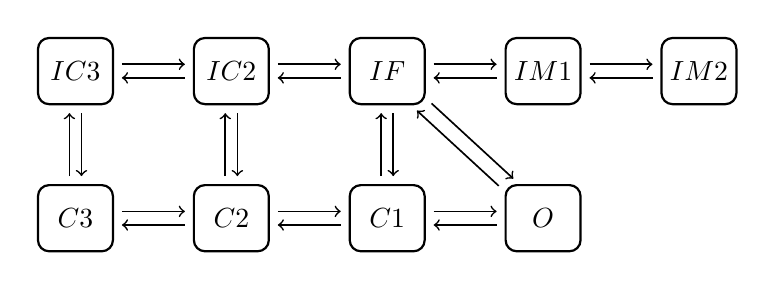
\begin{tikzpicture}[
   font=\sffamily,
   every matrix/.style={ampersand replacement=\&,column sep=1cm,row sep=1cm},
   state/.style={draw,thick,rounded corners,inner sep=.3cm},
   to/.style={->,semithick,shorten >=0.1cm,shorten <=0.1cm},
   Q/.style={->,semithick,sloped,pos=0.700000,shorten >=0.1cm,shorten <=0.1cm},  
   every node/.style={auto}]
\matrix{
\node[state] (IC3) {\parbox{10pt}{\centerline{$IC3$}}};\&\node[state] (IC2) {\parbox{10pt}{\centerline{$IC2$}}};\&\node[state] (IF) {\parbox{10pt}{\centerline{$IF$}}};\&\node[state] (IM1) {\parbox{10pt}{\centerline{$IM1$}}};\&\node[state] (IM2) {\parbox{10pt}{\centerline{$IM2$}}};\\
\node[state] (C3) {\parbox{10pt}{\centerline{$C3$}}};\&\node[state] (C2) {\parbox{10pt}{\centerline{$C2$}}};\&\node[state] (C1) {\parbox{10pt}{\centerline{$C1$}}};\&\node[state] (O) {\parbox{10pt}{\centerline{$O$}}};\&\\
};
\draw[to]  (IC3.10) to node {$$} (IC2.170);
\draw[to]  (IC3.280) to node {$$} (C3.80);
\draw[to]  (IC2.190) to node {$$} (IC3.350);
\draw[to]  (IC2.10) to node {$$} (IF.170);
\draw[to]  (IC2.280) to node {$$} (C2.80);
\draw[to]  (IF.190) to node {$$} (IC2.350);
\draw[to]  (IF.10) to node {$$} (IM1.170);
\draw[to]  (IF.280) to node {$$} (C1.80);
\draw[Q]  (IF.325) to node {$$} (O.125);
\draw[to]  (IM1.190) to node {$$} (IF.350);
\draw[to]  (IM1.10) to node {$$} (IM2.170);
\draw[to]  (IM2.190) to node {$$} (IM1.350);
\draw[to]  (C3.100) to node {$$} (IC3.260);
\draw[to]  (C3.10) to node {$$} (C2.170);
\draw[to]  (C2.100) to node {$$} (IC2.260);
\draw[to]  (C2.190) to node {$$} (C3.350);
\draw[to]  (C2.10) to node {$$} (C1.170);
\draw[to]  (C1.100) to node {$$} (IF.260);
\draw[to]  (C1.190) to node {$$} (C2.350);
\draw[to]  (C1.10) to node {$$} (O.170);
\draw[Q]  (O.145) to node {$$} (IF.305);
\draw[to]  (O.190) to node {$$} (C1.350);
\end{tikzpicture}
\end{center}
\caption{The sodium channel model of Clancy et al. \cite{Clancy2002}\label{clancy}; O is the open state, C1, C2 and C3 are the closed states, while the rest of the states represent different kinds of inactivation.}
\end{figure}
%{\it Glenn: forklar hva IM1, IM2 osv betyr i dette skjemaet.}

The popularity of these models stems from the fact that it is possible to adjust the parameters involved to obtain a model that reflects data quite well. However, it should also be mentioned that models can be so complex that it is virtually impossible to uniquely determine all the parameters involved. In these notes, we shall confine ourselves to relatively simple Markov models but the methods we describe can be applied, at least in principle, to Markov models of higher complexity.


\subsection{The master equation \label{master_equation}}

From the Markov model written on the form (\ref{Markov1}), we can derive an equation
giving the evolution of the probability of the two states, open (O) and closed (C). Let $o=o(t)$ be the
probability that the channel is in the open (O) state at time $t$ and let $c=c(t)$ denote
the probability that the channel is closed (C). We assume that the probabilities $o$ and $c$ are known at time
$t$ and then use the Markov model (\ref{Markov1}) to compute the probabilities at time $t+\Delta t$.
 Here $\Delta t$ is assumed to be so small that the channel changes state at most once during the time step from $t$ to $t+\Delta t$.   Then the scheme (\ref{Markov1}) states that
the open probability at time $t+\Delta t$ is given by%
\begin{align}
o(t+\Delta t) &= \text{Prob}\left[  (S(t)=C)  \mbox{\ and\ }  (C\rightarrow O \mbox{\ during\ } \Delta t)  \right] \\
& \ \ \ \ + \text{Prob}\left[  (S(t)=O)  \mbox{\ and not}  (O\rightarrow C \mbox{\ during\ } \Delta t)  \right] \\
&= c(t) \cdot (\Delta t k_{co}) + o(t) \cdot (1 -\Delta t k_{oc})
\end{align}
so
\[
o(t+\Delta t)=o(t)+\Delta t ( k_{co}c(t)-k_{oc}o(t)).
\]
%which expresses the fact that, during the time step from $t$ to $t+\Delta t$, the channel either remain open (first term), it changes from open to close (second term) or it changes from closed to open (last term).
From this equation, we obtain
\[
\frac{o(t+\Delta t)-o(t)}{\Delta t}=k_{co}c(t)-k_{oc}o(t),
\]
and, therefore, by passing to the limit $\Delta t\rightarrow0,$ we get the
differential equation%
\begin{equation}
o^{\prime}(t)=k_{co}c(t)-k_{oc}o(t).\label{po}%
\end{equation}
Similarly, we find that the probability of being in the closed state evolves
according to%
\begin{equation}
c^{\prime}(t)=k_{oc}o(t)-k_{co}c(t).\label{pc}%
\end{equation}
Since we are dealing with probabilities, it is reasonable to assume that the
initial conditions add up to one (the channel is either open or closed) and therefore, by adding the equations
above, we find that%
\[
o(t)+c(t)=1
\]
for all time. Hence the variable $c$ in $\left(  \ref{po}\right)  $ can be
replaced by $1-o$ and the system $\left(  \ref{po},\ref{pc}\right)  $ can be
written as a scalar equation of the form%
\begin{equation}
o^{\prime}(t)=\left(  k_{co}+k_{oc}\right)  \left(  \frac{k_{co}}%
{k_{co}+k_{oc}}-o\left(  t\right)  \right)  .\label{po2}%
\end{equation}
Here we see that
\[
o=\frac{k_{co}}{k_{co}+k_{oc}}%
\]
is a stable equilibrium solution. Furthermore, if we know that the channel is
closed initially, that is, $o(0)=0,$ we get the solution%
\[
o(t)=\frac{k_{co}}{k_{co}+k_{oc}}\left(  1-e^{-\left(  k_{co}+k_{oc}\right)
t}\right)
\]
and we notice that the equilibrium is reached more quickly as the sum of the rates
$k_{co}+k_{oc}$ increases.

\subsection[Three state model]{The master equation of a three-state model}

The development of the master equation for the two-state model above can be
carried out for any Markov model. For instance, if we consider the three-state
Markov model shown in Figure \ref{IOC_me}, we realize that the probabilities of the
open (O), closed (C), and inactivated (I) states are governed by the following system of ordinary
differential equations:
\begin{align}
o^{\prime}  & =k_{io}i+k_{co}c-\left(  k_{oi}+k_{oc}\right)  o, \nonumber \\
c^{\prime}  & =k_{oc}o+k_{ic}i-\left(  k_{co}+k_{ci}\right)  c,\label{me_11}\\
i^{\prime}  & =k_{oi}o+k_{ci}c-\left(  k_{io}+k_{ic}\right)  i, \nonumber
\end{align}
Since%
\begin{equation}
i=1-\left(  o+c\right),
\end{equation}
we have the following $2 \times 2$ system:%
\begin{align}
o^{\prime}  & =k_{io}+\left(  k_{co}-k_{io}\right)  c-\left(  k_{oi}%
+k_{oc}+k_{io}\right)  o,\label{me_20}\\
c^{\prime}  & =k_{ic}+\left(  k_{oc}-k_{ic}\right)  o-\left(  k_{co}%
+k_{ci}+k_{ic}\right)  c.\label{me_21}%
\end{align}
We will now show, using a numerical computation, that the solution of the
system (\ref{me_20},\ref{me_21}) coincides with the average result of Monte Carlo simulations using
the Markov model shown in Figure \ref{IOC_me} as the number of Monte Carlo runs goes
to infinity. 



\begin{figure}[ptb]
\begin{center}
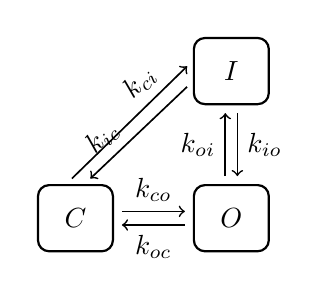
\begin{tikzpicture}[
   font=\sffamily,
   every matrix/.style={ampersand replacement=\&,column sep=1cm,row sep=1cm},
   state/.style={draw,thick,rounded corners,inner sep=.3cm},
   to/.style={->,semithick,shorten >=0.1cm,shorten <=0.1cm},
   Q/.style={->,semithick,sloped,pos=0.700000,shorten >=0.1cm,shorten <=0.1cm},  
   every node/.style={auto}]
\matrix{
\&\node[state] (I) {\parbox{10pt}{\centerline{$I$}}};\\
\node[state] (C) {\parbox{10pt}{\centerline{$C$}}};\&\node[state] (O) {\parbox{10pt}{\centerline{$O$}}};\\
};
\draw[to]  (O.100) to node {$k_{oi}$} (I.260);
\draw[to]  (O.190) to node {$k_{oc}$} (C.350);
\draw[to]  (I.280) to node {$k_{io}$} (O.80);
\draw[Q]  (I.195) to node {$k_{ic}$} (C.75);
\draw[to]  (C.10) to node {$k_{co}$} (O.170);
\draw[Q]  (C.105) to node {$k_{ci}$} (I.165);
\end{tikzpicture}
\end{center}
\caption{Markov model including three possible states: open (O), closed (C), and
inactivated (I).}%
\label{IOC_me}%
\end{figure}




\subsection[Monte Carlo Simulations]{Monte Carlo simulations based on the Markov model \label{MCSMM}}

Before we compare the two computational schemes, let us briefly describe how
the Monte Carlo simulation can be implemented. We choose a small timestep
$\Delta t$ and we assume that the state at time $t=t_{n}=n\Delta t,$ where $n$
is a non-negative integer, is either O, C, or I. For simplicity, we describe how
the computation proceeds in the case of the channel being in the open (O)
state at time $t=t_{n}$. In order to decide the state at time $t_{n+1}=t_{n}+\Delta t,$ we
divide the unit interval into three non-overlapping parts:  $A_{c}=\left[
0,k_{oc}\Delta t\right)  ,$ $A_{i}=\left[  k_{oc}\Delta t,k_{oc}\Delta
t+k_{oi}\Delta t\right)  ,$ $A_{o}=\left[  k_{oc}\Delta t+k_{oi}\Delta
t,1\right]  .$ Then, at time $t_{n+1}=t_{n}+\Delta t,$ we can update the state
of the channel based on a random number $r_{n}$ in the unit interval drawn from
a uniform distribution. Specifically, if $r_{n}\in A_{o},$ the channel
remains open; if $r_{n}\in A_{c},$ the state of the channel changes from
open to closed; and, finally, if $r_{n}\in A_{i},$ the state of the channel
changes from open to inactivated. 

Similar steps are straightforward to
devise for the case of the channel being in the closed or inactivated states
at time $t=t_{n}.$ 

%\GTL{Perhaps mention here that for this simple case (rates not varying in time) the Gillespie method is much more efficient.} 

\subsection[Monte Carlo simulation vs Master Equation]{Comparison of Monte Carlo simulations and solutions of the
master equation}

In Figure \ref{Introduction_L/ode_mc.pdf} we compare the probabilities computed by solving the master equation $\left( \ref{me_20},\ref{me_21}\right)  $ (red lines) and by Monte Carlo simulations using the Markov model as described above. In the simulations we have used the initial conditions $o(0)=i(0)=0$
and $c(0)=1$ and the rates used in the computations are given in Table \ref{tab:const3x3}. As the number of Monte Carlo simulations increases, we see that the average approaches the solution of the continuous master equation. In these computations the master equation was solved using the function \GTLV{ODE15s in Matlab}.


\begin{table}  \begin{center}                            
\begin{tabular}{|r|r|r|r|r|r|} \hline                    
$k_{oi}$ & $k_{io}$ & $k_{co}$ & $k_{oc}$ & $k_{ic}$ &$k_{ci}$  \\ \hline    
0.5  &    0.3 &   0.6   &  0.9  &   0.72  & 0.8 \\ \hline    
\end{tabular} \end{center}                               
\caption{Rates (in 1/ms) of the Markov model given in Figure  \ref{IOC_me} used in the computations presented in Figure \ref{Introduction_L/ode_mc.pdf}.}
 \label{tab:const3x3}  \end{table}                                              


%xxGlenn: Lag gjerne 3x3 paneler, der o,c,og i g\aa r fra venstre mot h\o yre og der antall MC \o ker (og dt reduseres) ovenfra og ned. Alle detaljer i caption og i tabellene nevnt over.

\fig[0.9]{Introduction_L/ode_mc.pdf}{ Comparison of the solution of the master equation $\left( \ref{me_20},\ref{me_21}\right)$ (red lines) and the results of Monte Carlo simulations based on the Markov model given in Figure \ref{IOC_me}. The time step used in the Monte-Carlo simulations was $\Delta t$ = 0.01 ms in all the panels and the simulations were run for 10 ms. The number of Monte Carlo simulations increases from 100 (top) to 10,000 (bottom).}


\subsection{Equilibrium probabilities \label{eq_prob_ioc}}

The equilibrium state of the
reaction shown in Figure  \ref{IOC_me} is characterized by the equations%
\begin{align}
k_{co}c  &  =k_{oc}o, \nonumber\\
k_{oi}o  &  =k_{io}i, \label{me_eq_20}\\
k_{ic}i  &  =k_{ci}c, \nonumber
\end{align}
where $o,c,$ and $i$ denote the probabilities of the channel being open,
closed, or inactivated, respectively. It follows that%
\[
c=\frac{k_{oc}}{k_{co}}o
\]
and
\[
i=\frac{k_{oi}}{k_{io}}o.
\]
By using the fact that $o+c+i=1,$ we obtain
\[
\left(  1+\frac{k_{oc}}{k_{co}}+\frac{k_{oi}}{k_{io}}\right)  o=1
\]
and therefore%
\begin{align*}
o  &  =\frac{1}{1+\frac{k_{oc}}{k_{co}}+\frac{k_{oi}}{k_{io}}},\\
c  &  =\frac{\frac{k_{oc}}{k_{co}}}{1+\frac{k_{oc}}{k_{co}}+\frac{k_{oi}%
}{k_{io}}},\\
i  &  =\frac{\frac{k_{oi}}{k_{io}}}{1+\frac{k_{oc}}{k_{co}}+\frac{k_{oi}%
}{k_{io}}}.
\end{align*}
For the particular rates given in Table \ref{tab:const3x3}, we get the following equilibrium probabilities: $o=0.24,\, c=0.36$, and
$i=0.4$.

\subsection{Detailed balance}

In order to compute the equilibrium solution of (\ref{me_11}) above, we assumed that each of the sub-transitions of the diagram given in Figure \ref{IOC_me} was in equilibrium. More precisely, we assumed that
\[k_{co}c    =k_{oc}o, \, k_{oi}o =k_{io}i,  \text{ and }k_{ic}i =k_{ci}c. \]
These three relations yield
\begin{equation}
k_{co}k_{oi}k_{ic}=k_{ci}k_{io}k_{oc}. \label {db}
\end{equation}
This relation is referred to as the condition of {\it detailed balance}. In these notes, we will always assume that Markov models satisfy this condition. More generally, the product of the rates in a loop (e.g. the I-O-C loop of Figure \ref{IOC_me}) in the clockwise direction equals the product of the rates in the counterclockwise direction. Under this assumption, the equilibrium solution can always be computed by the method indicated above. We will use the same technique many times in these notes.



\section{The master equation and the equilibrium solution \label{me_eq}}

We have seen that the Markov model written in the form
\begin{equation}
C\underset{k_{co}}{\overset{k_{oc}}{\leftrightarrows}}O \label{Markov1010}%
\end{equation}
leads to a master equation of the form 
\begin{align}
o^{\prime}(t)=  &  k_{co}c(t)-k_{oc}o(t),\label{po1010}\\
c^{\prime}(t)=  &  k_{oc}o(t)-k_{co}c(t). \label{pc1010}%
\end{align}
Since $o+c=1,$ we can reduce the system to the scalar equation,%
\[
o^{\prime}(t)=\left(  k_{co}+k_{oc}\right)  \left(  \frac{k_{co}}%
{k_{co}+k_{oc}}-o\left(  t\right)  \right)
\]
and we readily see that the equilibrium solution is given by
\[
o=\frac{k_{co}}{k_{co}+k_{oc}}.
\]
Exactly the same steps can be followed for the three-state Markov model
illustrated in Figure \ref{IOC_me}. The associated Markov model reads
\begin{align*}
o^{\prime} &  =k_{io}i+k_{co}c-\left(  k_{oi}+k_{oc}\right)  o\\
c^{\prime} &  =k_{oc}o+k_{ic}i-\left(  k_{co}+k_{ci}\right)  c\\
i^{\prime} &  =k_{oi}o+k_{ci}c-\left(  k_{io}+k_{ic}\right)  i
\end{align*}
and since
\begin{equation}
i=1-\left(  o+c\right)  \label{i4010}%
\end{equation}
we arrive at the following $2 \times 2$ system:%
\begin{align*}
o^{\prime} &  =k_{io}+\left(  k_{co}-k_{io}\right)  c-\left(  k_{oi}%
+k_{oc}+k_{io}\right)  o,\\
c^{\prime} &  =k_{ic}+\left(  k_{oc}-k_{ic}\right)  o-\left(  k_{co}%
+k_{ci}+k_{ic}\right)  c.
\end{align*}
The equilibrium solution is now defined by a $2 \times 2$ linear system of equations of
the form%
\begin{equation}
Bq=b,\label{i4011}%
\end{equation}
where
\[
B=\left(
\begin{array}
[c]{cc}%
k_{oi}+k_{oc}+k_{io} & k_{io}-k_{co}\\
k_{ic}-k_{oc} & k_{co}+k_{ci}+k_{ic}%
\end{array}
\right)  ,\;q=\left(
\begin{array}
[c]{c}%
o\\
c
\end{array}
\right)  \text{, and }b=\left(
\begin{array}
[c]{c}%
k_{io}\\
k_{ic}%
\end{array}
\right)  .\;
\]
By solving this linear system and using $\left(  \ref{i4010}\right)$, we
find (as above) that%

\[
o=K^{-1},\;c=\;\frac{k_{oc}}{k_{co}}K^{-1},\;i=\frac{k_{oi}}{k_{io}}K^{-1},%
\]
where%
\[
K=1+\frac{k_{oc}}{k_{co}}+\frac{k_{oi}}{k_{io}}.
\]

\subsection[Linear algebra]{Linear algebra approach to finding the equilibrium solution}

Calculations to find the equilibrium solution will be done repeatedly in these notes. We
will always use the special structure of the Markov model to derive the
equilibrium solution, but it also worth noting that this can be done by
solving a linear system. The master equation associated with a Markov model of the
form  $\left(  \ref{Markov1010}\right)$ or of the form given in
Figure \ref{clancy} can always be written in the form%
\[
p^{\prime}=Ap,
\]
where $p$ is a vector containing the probabilities of occupying the different
states of the Markov model. Since the sum of the probabilities adds up to one,
the number of unknowns can be reduced by one and the system takes the form%
\[
q^{\prime}=b-Bq.
\]
Therefore, the equilibrium solution can be found by solving the linear system
$\left(  \ref{i4011}\right)  .$

Instead of reducing the number of unknowns, we can also address the problem more directly by computing the eigenvector
associated the eigenvalue $\lambda = 0$. For instance, using Matlab  we can put $z=\rm{null}(A)$ and then define 
\[p=\frac{z}{\sum_i z_i}\]
 where
$z_i$ denote the components of the vector $z$.


\section[Stochastic simulations and PDFs]{Stochastic simulations and probability density functions}

Given the Markov model, defining a stochastic differential equation describing changes of the transmembrane potential due to the opening and closing of the channel is quite straightforward. Additionally, based on the stochastic differential equation, we will derive deterministic differential equations describing the probability density functions of the states involved in the Markov model. We thus have two ways to analyze models of ion channels: We can either run numerous Monte Carlo simulations using the stochastic differential equation or solve the deterministic differential equations defining the probability density functions. Both these methods will be used throughout the notes. Although one method is the average of the other, we will see that both provide distinct insights useful to understanding the mechanisms under consideration. 


\section{Markov models of calcium release}
The contraction of the heart is a collective and very well-coordinated effort achieved in a collaboration involving billions of cells. For each of these cells, the contraction depends on the release of a massive amount of calcium from internal storage. The release takes place in many thousands of release units within each cell and the state of the release process is believed to be adequately modeled using Markov models. 

We will study this release in several steps and we start by assuming that the only varying concentration is in the dyad and that the reaction rates of the Markov model vary only with this single concentration. This case will be studied in great detail and we will explain how drugs can be theoretically constructed to repair mutations affecting the release mechanism. The analysis is based on a scalar stochastic differential equation representing the concentration of calcium in the dyad. The properties of this model will be analyzed using Monte Carlo simulations. Furthermore, we will derive a system of deterministic partial differential equations describing the probability density function of the states of the Markov model. 

It is more common to divide the calcium concentration into two values---not only one---which leads to  $2\times2$ stochastic differential equations to be analyzed. This model will also be analyzed using Monte Carlo simulations and by a 2D deterministic system of partial differential equations representing the probability density functions of the states of the Markov model.

Next, we shall couple the calcium concentration to the voltage-gated release of calcium through so-called L-type calcium channels. This model will allow us to study optimal drugs, combining the effect on calcium release and L-type channels. The balance of these mechanisms rules the calcium-induced calcium release that is at the crux of cardiac contraction. The calcium-induced calcium release model is stated in terms of a $2\times 2$ model of stochastic equations where the transmembrane potential $V$ is included as a parameter in the model. The associated model for the probability density functions is given by a 2D system of partial differential equations where the transmembrane potential is again included as a parameter.
 
 \section{Markov models of ion channels}
 
After analysis of the calcium release we move on to study voltage-gated  ion channels. We will immediately see that in mathematical terms the problem is very similar to the calcium release problem. For the ion channel case, however, the stochastic equation is one-dimensional and so is the associated deterministic partial differential equation. The basic Markov model is still based on the open and closed states, but we will also see that an inactivated state plays a central role. Optimal theoretical drugs will be derived and we will observe that they work nicely.

\section{Mutations described by Markov models}

A trademark of mutations affecting ion channels and calcium release mechanisms is that they change the open probability and possibly also the mean open time and other characteristics of the channels involved. We will show below that the equilibrium open probability of the channel described by the Markov model of the form (\ref{Markov1}) is given by 
\[ o=\frac{k_{co}}{k_{co}+k_{oc}} \]
and the mean open time is given by
\[ \tau_o=\frac{1}{k_{oc}}. \]
The concept of mean open time will be discussed in Chapter \ref{mot_chapter} and the formula $\tau_o=1/k_{oc}$ will be derived in that chapter.
 Given these formulas, it is straightforward to see that the effect of mutations affecting the open probability or the mean open time can be modeled by changing the parameters of the Markov model. In these notes we shall focus on rather simple changes 
 in the model but, again, the techniques can be generalized to more intricate cases.
 
  Two examples of the effect of mutations are given in Figures 
 \ref{Introduction_L/Loaiza_crop.png}  and \ref{Introduction_L/chandra.png}. Figure
 \ref{Introduction_L/Loaiza_crop.png}  shows recordings of the open and closed states for the wild type and the 
  V2475F mutation of the ryanodine receptor (RyR).
  The graphs in Figure \ref{Introduction_L/chandra.png} show similar results for the voltage-gated sodium channel when the wild type recordings are compared with recordings from a mutant ($\Delta$KPQ) channel.


\fig[0.5]{Introduction_L/Loaiza_crop.png}{Single-channel recordings of wild type (black) and mutant (red) cardiac RyR channels. The open probability and the mean open time are significantly increased for the mutant (V2475F) case. The graphs are from Figure 3 of Loaiza et al. \cite{loaiza2013}.}

\fig[0.9]{Introduction_L/chandra.png}{Sodium current recordings taken from Figure 4 of Chandra et al. \cite{Chandra1998}: A represents the wild type and B represents 
the $\Delta$KPQ mutant. The recordings are based on 200-ms depolarizing pulses from -100 mV to -40 mV. }


\section{The problem and steps toward solutions}

Assume that experimental data on wild type cells can be used to identify the parameters of a Markov model faithfully describing the stochastic properties of the wild type channel and that experimental data on mutant cells can be used to establish a Markov model of similar structure representing the stochastic properties of the mutant channel. Furthermore, we assume that the Markov model of the mutant can be extended to account for the effect of a theoretical drug. {\it The problem is then to compute the reaction rates of the drug such that, after the drug is applied, the mutant channel behaves as similarly to the wild type channel as possible. } The essence of these notes is to show how to solve this problem mathematically; we show how to compute an optimal theoretical drug. To clarify what we mean by an optimal theoretical drug, we will give a few examples that will be discussed later and then we will briefly discuss the concept of a theoretical drug  more generally.

 \subsection{Markov models for drugs: Open state and closed state blockers}
 By using the notation of chemical reactions introduced above, we can explain the problem in a bit more detail. The reaction scheme for an open state blocker can be illustrated as follows:
\begin{equation}
C\underset{ k_{co}}{\overset{k_{oc}}{\leftrightarrows}}O\underset{k_{ob}%
}{\overset{k_{bo}}{\leftrightarrows}}B. \label{open_block}
\end{equation}
For theoretical purposes, this drug is well defined, provided that we know the values of the parameters $k_{ob}$ and $k_{bo}$. We will often assume that these parameters are constants. As mentioned above, one example of a problem we want to overcome
is mutations leading to an increased open probability; so either the release mechanism is too prone to releasing calcium from internal storage or the ion channels are too prone to allowing  current to flow through the cell membrane. 

Since the problem involves too high of an open probability, it seems reasonable to try to fix the open probability by extending the reaction scheme and directly affecting this state, as illustrated in the reaction scheme above. By allowing the probability to be moved from $O$ to $B$, the open probability will be reduced and thus the goal will be achieved. This reasoning seems impeccable and it seems much less intuitive to use a closed state drug of the form
\begin{equation}
B\underset{k_{bc}}{\overset{k_{cb}}{\leftrightarrows}}C\underset{
k_{co}}{\overset{k_{oc}}{\leftrightarrows}}O. \label{closed_block}
\end{equation}
We will see, however, that both open and closed state blockers may be optimal, depending on the nature of the mutation.

\subsection{Closed to open mutations (CO-mutations) \label{com}}
We have seen that for a Markov model written in the form
\begin{equation}
C\underset{ k_{co}}{\overset{k_{oc}}{\leftrightarrows}}O,
\end{equation}
 the equilibrium open probability is given by
\[ o=\frac{k_{co}}{k_{co}+k_{oc}}=\frac{1}{1+\frac{k_{oc}}{k_{co}}} \]
and the mean open time is given by
\[ \tau_o=\frac{1}{k_{oc}}. \]
A mutation leading to an increased open probability can be represented by a Markov model written in the form
\begin{equation}
C\underset{ \mu k_{co}}{\overset{k_{oc}}{\leftrightarrows}}O,
\end{equation}
where $\mu \ge 1$ will be referred to as the {\it mutation severity index} and we always use the convention that $\mu=1$ refers to the wild type case. At this point, it is useful to recall the interpretation of a scheme of this form. In particular, it is useful to note that the probability of going from the closed state (C) to the open state (O) during a time step $\Delta t$ is now given 
by $\mu \Delta t k_{co}$, compared to $\Delta t k_{co}$ for the wild type channel. It is pretty clear that increasing the mutation severity index will increase the probability of being in the open state and this is also reflected by the equilibrium open probability given by
\[o_\mu=\frac{1}{1+\frac{k_{oc}}{\mu k_{co}}}, \]
which clearly increases as a function of the mutation severity index $\mu$. 
It is also interesting to observe that, for this mutation, the mean open time is unchanged. We will refer to a mutation of this form as a CO-mutation and we will show repeatedly that, for CO-mutations, closed state blockers are theoretically optimal.

\subsection{Open to closed mutations (OC-mutations)}
Another way to introduce a mutation that increases the open probability is to decrease the rate from open to closed. This can be written as follows:
\begin{equation}
C\underset{ k_{co}}{\overset{k_{oc}/\mu}{\leftrightarrows}}O,
\end{equation}
where, again, $\mu \ge 1$ is the mutation severity index and $\mu=1$ represents the wild type. The probability of leaving the open state is now reduced and this will lead to an increased open probability.
In particular, the equilibrium open probability is again given by
\[ o_\mu=\frac{1}{1+\frac{k_{oc}}{\mu k_{co}}}, \]
as above, but now the mean open time changes; it is given by
\[ \tau_o=\frac{\mu}{k_{oc}}\]
and thus increases with the mutation severity index.

We will refer to a mutation of this form as an OC-mutation and we will show that, for such mutations, open state blockers are theoretically optimal.

\section{Theoretical drugs \label{theoreticaldrugs}}

The concept of a theoretical drug is essential in these notes. Basically, we will {\em  refer to a theoretical drug\footnote{We also use the terms \textit{mathematical drug, numerical drug}, and so forth interchangeably with \textit{theoretical drug}} as a purely mathematical construction} that may or may not have a viable pharmaceutical counterpart. A mental image of how the drug may work is given in Figure \ref{Introduction_L/drg_starmer.png}; the figure is taken from Starmer \cite{Starmer2002}. With no drug involved, the channel can take on two conformational states: the open state (O), when ions can flow freely through the channel, and the closed state (C), when there is no flow of ions through the channel. An open blocker can change the open state such that there is no flow through the channel. The reaction scheme of the situation described in the figure is given by
\begin{equation}
C\underset{ k_{co}}{\overset{k_{oc}}{\leftrightarrows}}O\underset{k_{ob}%
}{\overset{k_{bo}}{\leftrightarrows}}B. \label{closed_block201}
\end{equation} where we again note that the properties of the theoretical drug are solely given by the values of the rates $k_{ob}$ and $k_{bo}$. 

This way of describing the effect of a drug has been used for many years, see e.g. Hille \cite{Hille1977} or Hondeghem and Katzung \cite{Hondeghem1977}. Our use of this notation is clearly motivated by the paper of Clancy et al. \cite{Clancy2007}. In these papers, an existing drug is characterized using a scheme of the form (\ref{closed_block201}). That is, data obtained from experiments using a particular drug are used to characterize the rates $k_{bo}$ and $k_{ob}$ referred to, respectively, as the on and off rates of the drug. As mentioned above, we often view the rates as free parameters that can be optimized in order to create the best possible theoretical drug in the sense that the channel should work as much like the healthy case as possible. This way of describing a theoretically optimal drug was introduced in \cite{Tveito2011c} and clearly motivated by the drug vector approach discussed in   \cite{Tveito2009}.

\fig{Introduction_L/drg_starmer.png}{Illustration of a blocker associated with the open state. In the leftmost case the channel is closed and no ions can pass through it. In the center case, the channel is open and ions may flow freely. In the rightmost case the channel is blocked by the drug and no ions can pass through it. The figure is taken from Starmer \cite{Starmer2002}.}

\section{Results}
Many of the models, methods, and results described in these notes are well known in the literature. All the Markov models are taken from the literature and so are the stochastic differential equations and the models describing the probability density approach. Compared to earlier published models, we will often derive simplified models, but the ideas behind them are basically the same as those used by many authors. Concerning the modeling of mutations, we aim to consistently model the effect of mutations as simply as possible and preferably only by changing a single parameter: the mutation severity index. 

The novel part of these notes is that we attempt to systematically describe how to compute characterizations of drugs that are optimal in a specific sense and we do so for a number of applications. We almost exclusively address so-called gain-of-function mutations. For such mutations, the open probability of the channel or receptor is too large, which can lead to severe difficulties for the cell and, ultimately, for large collections of such cells. 

%We begin by studying such mutations in cases where the mean open time is unaltered. In such cases, we give several examples indicating that closed blockers are much better suited for repairing the effect of the mutation than open blockers. If, on the other hand, both the open probability and the mean open time is affected, open state blockers are to be preferred. In a similar manner we discuss how to deal with mutations that impair the inactivation of ion channels.

\section{Other possible applications}

The focus in this text will be on how to compute characterizations of optimal theoretical drugs defined in terms of parameters describing the associated Markov model. The methods can, however, also be used to compare existing drugs. If Markov models are developed for two drugs, the associated probability density functions can be computed and thus a comparison of the quality of the two drugs can be computed. This approach will rely heavily on accurate representations of the function of a drug in terms of a Markov model, which is a problem beyond the scope of the present notes.


\section{Disclaimer}
These notes are written to explain in some detail how we can compute characterizations of theoretical drugs in terms of Markov models. However, we specifically avoid discussing whether it is possible to realize a certain drug given the characterization in terms of a Markov model, simply because we do not know and have been unable to find any reasonable answer to this in the literature.  The applicability of our results therefore remains uncertain.


\section{Notes}
\begin{enumerate}
\item Several excellent introductions to Markov models of the stochastic behavior of receptors and ion channels are available (e.g., \cite{KeenerSneyd, Smith2002, Jacobs2010, Santillan2014}). In particular we recommend the recently published book by Bressloff \cite{Bressloff2014} (see also \cite{Bressloff2014w}). Bressloff \cite{Bressloff2014} provides a broad introduction to stochastic processes in cells and covers most of the models covered in the present text and much more. It is an excellent text that will become a standard reference in the field.
\item A comprehensive mathematical analysis of the stochastic properties of single ion channels using Markov models was initiated by Colquhoun and Hawkes (e.g., \cite{ Colquhoun1977,Colquhoun1981,Colquhoun1982}).
\item Insight into the electrophysiology of excitable cells was fundamentally enhanced by the development of the patch clamp technique of Sakmann and Neher (see, e.g., \cite{Sakmann1984,Sakmann1995}). The authors received the Nobel Prize in Physiology or Medicine in 1991 for their work on single ion channels. The patch clamp technique is used to generate measurements of the form illustrated in 
Figure \ref{Introduction/na_cropped.png}. These data are used to determine the Markov model and are therefore of fundamental importance. As mentioned below, however, the problem of finding the Markov model based on experimental data is still an active research problem.
\item The models studied in these notes address the flow of ions through various types of channels. An excellent introduction to ion channels is given in the book by Hille \cite{Hille2001}.
\item Our discussion is focused on mechanisms of the heart but, at the level of single channels, these mechanisms are similar to channel-based mechanisms of the brain or, more specifically, the mechanisms of neurons. There are several excellent introductions to neuroscience  
(e.g., \cite{Ermentrout2010,Sterratt2011,Dayan2001,Izhikevich2007}).
\item 
Given the Markov model, we have seen that it is pretty straightforward to compute what state the channel is in as a stochastic function of time. We have also seen that we can solve the master equation and find the average behavior of the channel when the rates are independent of the surroundings. Furthermore, we will show how to compute probability density functions for each state when the rates depend on the transmembrane potential. Such simulations are forward problems: Given the model,  compute the solution. The inverse problem in this setting is quite a bit harder; the problem is to compute the rates (i.e., the values of $k_{oc},\,  k_{co}$ etc.) of the Markov model in order for the stochastic behavior of the model to match the measurements of the channel. The analysis of the inverse problem was started by Colquhoun and Hawkes \cite{Colquhoun1977}, beginning in 1977, and their findings are summarized by Sakmann and Neher \cite{Sakmann1995} (see also
\cite{Colquhoun1996}). More recently the problem has been addressed in a series of papers by Sachs and his co-authors; see \cite{Qin1996,Qin2000,Nicolai2013}. Their methods are available in the open-source QuB software package. Furthermore, Markov chain Monte Carlo (MCMC) has been used in a series of papers by Siekmann, Sneyd and his co-authors \cite{Gin2009,Siekmann2011,Siekmann2012, Siekmann2014}. Interestingly, their analysis shows that certain Markov models cannot be identified using standard data. The MCMC method was used for inversion of single ion channel data more than 15 years ago by Ball et al \cite{Ball1999}, and Rosales and co-authors, see \cite{Rosales2001,Rosales2004}.
\item For whole cell data, the problem of identifying the parameters of Markov models is carefully studied by Fink and Noble \cite{Fink2009}. 
\item The terms {\it CO-mutation}, {\it OC-mutation}, and {\it mutation severity index} are not standard and introduced here for convenience. 
\item A thorough discussion of the principle of detailed balance can be found in the paper by  Colquhoun et al. \cite{Colquhoun2004}. The validity of the principle for given data can be tested as shown by Song and Magleby \cite{Song1994} and Ullah et al. \cite{Ullah2012} (suppl. material).
There are examples of Markov models that do not satisfy the principle of detailed balance (see, e.g., \cite{Bressloff2014}, p. 208). 
\item The numerical method for handling the Markov model described on page \pageref{MCSMM} is not particularly efficient. For the case of constant rates in the Markov model, considerable acceleration can be achieved by using the method of Gillespie \cite{Gillespie1977}. The Gillespie method is particularly useful for simulations involving many channels (see, e.g., \cite{Smith2002}). 
\item For comprehensive introductions to modeling the cardiac action potential, we refer to the recent overview by Rudy \cite{Rudy2012} and to Rudy and Silva \cite{Rudy2006}.  For the action potential shown in Figure \ref{Introduction_L/grandi.pdf}, we used the model of Grandi et al. \cite{Grandi2010B}. An alternative is the model of O'Hara et al. \cite{Ohara2011} and a huge collection of models is available at the CellML project (CellML.org).
\item The dynamics of cardiac electrophysiology are introduced in numerous papers and books; a recent comprehensive review is provided by Qu et al. \cite{Qu2014}.  The book by Katz \cite{Katz2010} 
is a standard reference in cardiac physiology and the book by Glass et al. \cite{Glass2012} is a standard reference in the modeling of the heart. Numerical methods for the simulation of cardiac electrophysiology are presented by Sundnes et al. \cite{Sundnes2007} (see also \cite{Pullan2005, Franzone2014}). 

 

\end{enumerate}










\input{Ca_1D_L/Ca_release_1D}

\chapter{Properties of probability density functions}



The physical processes we study in this text are modeled using models including stochastic terms. Direct numerical simulations based on such stochastic models give results that are hard to interpret and it is therefore common to run many simulations and compute the average, and we have also seen that we can derive models governing the probability density functions. These are powerful tools that provide insight in the processes. In this chapter we will see that it is useful to have specific numbers that characterize
stochastic variables and associated probability density functions. We 
encountered the equilibrium probability of being in the open or closed state
(see, e.g., page \pageref{eq_pr_wt}) and we introduced probability density
functions (see, e.g., page \pageref{sec:pdf}). Here we shall derive some specific (and common)
characteristics of the probability density functions and discuss how these
characteristics can be used to gain an understanding of calcium release. We will
also show how the characteristics relate to the concepts already introduced 
and we will discuss how the characteristics vary as functions of the mutation
severity index. Finally, we will show how the statistical characterizations can be used 
to evaluate the properties of theoretical drugs.





\section{Probability density functions}


 Let us briefly recall the models under consideration. We consider the model
\begin{equation}
\bar{x}^{\prime}(t)=\bar{\gamma}(t)v_{r}(c_{1}-\bar{x})+v_{d}(c_{0}-\bar{x})
\label{asde1D100}
\end{equation}
of the calcium concentration of the dyad (see Figure \ref{cicr_1D}). Recall that $v_{r}$
denotes the speed of release from the sarcoplasmic reticulum (SR) to the dyad, $v_{d}$ denotes the speed of diffusion
from the dyad to the cytosol, $c_{0}$ is the concentration of calcium ions in
the cytosol, and $c_{1}$ is the calcium concentration in the SR; both $c_0$ and $c_1$ 
are assumed to be constant. The stochastic
function $\bar{\gamma}=\bar{\gamma}(t)$ can be either zero (closed state) or 
one (open state) and the state is governed by the Markov model

\begin{equation}
C\underset{k_{co}}{\overset{k_{oc}}{\leftrightarrows}}O, \label{M100}
\end{equation}
where $k_{oc}$ and $k_{co}$ are the rates associated with the Markov model. As
discussed above, the probability density functions of the states of the Markov
model are governed by the following system of partial differential equations:
\begin{align}
\frac{\partial\rho_{o}}{\partial t}+\frac{\partial}{\partial x}\left(
a_{o}\rho_{o}\right)   &  =k_{co}\rho_{c}-k_{oc}\rho_{o},\label{pdf1000}\\
\frac{\partial\rho_{c}}{\partial t}+\frac{\partial}{\partial x}\left(
a_{c}\rho_{c}\right)   &  =k_{oc}\rho_{o}-k_{co}\rho_{c}, \label{pdf1001}
\end{align}
where, as above, $\rho_{o}$ and $\rho_{c}$ are the probability density
functions of the open and closed states, respectively. Furthermore, we recall
that
\begin{align}
a_{o}  &  =v_{r}(c_{1}-x)+v_{d}(c_{0}-x),\label{aos}\\
a_{c}  &  =v_{d}(c_{0}-x). \label{acs}
\end{align}
The system of partial differential equations given by $\left(
\ref{pdf1000}\right)$ and (ref{pdf1001}) is solved on the computational
domain given by $\Omega=[c_0,c_+]$, where
\[
c_{+}=\frac{v_{r}c_{1}+v_{d}c_{0}}{v_{r}+v_{d}},
\]
and the boundary conditions are set up to ensure that there is no leak of probability across the
boundaries (see page \pageref{bc}).

\section{Statistical characteristics}
\label{statistics}

\bigskip For the probability density functions given by the system $\left(
\ref{pdf1000}\right)$ and (ref{pdf1001}), we can introduce the common statistical
concepts of probability, expectation, and standard deviation. The probabilities of
being in the open and closed states are given by
\begin{equation}
\pi_{o}=\int_{\Omega}\rho_{o}dx \text{ and }\pi_{c}=\int_{\Omega}\rho_{c}dx,
\label{probability}
\end{equation}
respectively. It is worth noting that these values are time dependent but
independent of space (concentration). Furthermore, the sum of these
probabilities adds up to one,
\[
\pi_{o}\left(  t\right)  +\pi_{c}\left(  t\right)  =1,
\]
for all time. The expected values of the concentration are given by
\begin{equation}
E_{o}=\frac{1}{\pi_{o}}\int_{\Omega}x\rho_{o}dx \text{ and }E_{c}=\frac{1}
{\pi_{c}}\int_{\Omega}x\rho_{c}dx \label{expectation}
\end{equation}
under the condition that the channels are open and closed, respectively. Finally, the standard deviations $\sigma_{o}$ and $\sigma_{c}$ are given by
\begin{align}
\sigma_{o}^{2}  &  =\frac{1}{\pi_{o}}\int_{\Omega}x^{2}\rho_{o}dx-E_{o}^{2},\label{stdvo}\\
\sigma_{c}^{2}  &  =\frac{1}{\pi_{c}}\int_{\Omega}x^{2}\rho_{c}dx-E_{c}^{2}. \label{stdvc}
\end{align}

We will show below how changes in the Markov model affect these
characteristics and how the characteristics are influenced by the
theoretical drugs. Generally, we have to solve the system $\left(
\ref{pdf1000}\right)$ and (ref{pdf1001}) and then compute the statistical
properties. However, we will see that in the special case in which the rate functions
defining the Markov model, $k_{oc}$ and $k_{co}$, are constant; we can compute some of
the characteristics analytically.  We will therefore start by considering such a case.



\section{Constant rate functions}
\graytable{l}{
{|c|c|} \hline
$v_d $ & 0.1 $\rm{ms^{-1}}$\\ \hline
$v_r $ & 1.0 $\rm{ms^{-1}}$\\ \hline
$c_0 $ & 0 $\rm{mM}$\\ \hline
$c_1 $ & 1 $\rm{mM}$ \\ \hline
$k_{co} $ & 1 $\rm{ms^{-1}}$ \\ \hline
$k_{oc} $ & 1 $\rm{ms^{-1}}$ \\ \hline
}{Parameter values for the model of (\ref{asde1D100}) and (\ref{M100}).
%\K{zzz $v_d$ og $v_r$ m\r{a} vel ha benevning $\rm{ms^{-1}}$ (istedenfor  $\rm{\mu M/ms}$) i Table \ref{tab:nodrug}, Table \ref{tab:xdep} og Table \ref{tab:nodrug_again} for at enhetene skal g\r{a} opp?}
\label{tab:nodrug}}
We consider the system (ref{pdf1000}) and (ref{pdf1001}) in the
special case that both $k_{oc}$ and $k_{co}$ are constants (independent of the concentration $x$). If we integrate
(ref{pdf1000}) and (ref{pdf1001}) over the interval $\Omega$, we obtain the system
\begin{align}
\pi_{o}^{\prime}  &  =k_{co}\pi_{c}-k_{oc}\pi_{o},\label{pi1}\\
\pi_{c}^{\prime}  &  =k_{oc}\pi_{o}-k_{co}\pi_{c}, \label{pi2}
\end{align}
where we use the boundary conditions that state that there is no flux
of probability across the boundaries.

\subsection{Equilibrium probabilities}


When this system reaches equilibrium, the probabilities satisfy
\begin{equation}
k_{co}\pi_{c}=k_{oc}\pi_{o}
\end{equation}
and since $\pi_{o}+\pi_{c}=1,$ we find that
\begin{align}
\pi_{o} &  =\frac{k_{co}}{k_{oc}+k_{co}},\label{eq_po}\\
\pi_{c} &  =\frac{k_{oc}}{k_{oc}+k_{co}},\label{eq_pc}
\end{align}
which we recognize as the probabilities $o$ and $c$, respectively, derived directly from the
equilibrium of the Markov model on page \pageref{eq_pr_wt}. This relation explains
the connection between these two ways of considering the probability of
being in a given state of the Markov model, but it is important to note that
this relation only holds when the rate functions are constant.

%\footnote{The case of constant values
%of the rate functions $k_{oc}$ and $k_{co}$  is quite important because of the experimental technique referred
%to as voltage clamping. The technique allows the current to be measured while the transmembrane potential is kept fixed. }.


\subsection{Dynamics of the probabilities}

In the special case with only two states of the Markov model and constant
rate functions, we can analytically compute how the probabilities evolve in
time. If we use the fact that $\pi_{o}\left(  t\right)  +\pi_{c}\left(
t\right)  =1$ for all time, we find that the system (ref{pi1})
and (ref{pi2}) can be reduced to one equation written in the form
\begin{equation}
\pi_{o}^{\prime}=\left(  k_{co}+k_{oc}\right)  \left(  \frac{k_{co}}
{k_{co}+k_{oc}}-\pi_{o}\right)  . \label{pi_o}
\end{equation}
Suppose we know that the channel is closed at $t=0;$ then $\pi_{o}(0)=0$ and
we find the solution
\begin{equation}
\pi_{o}(t)=\frac{k_{co}}{k_{co}+k_{oc}}\left(  1-e^{-\left(  k_{co}
+k_{oc}\right)  t}\right)  .\label{pio11}
\end{equation}
We note that if the channel is closed at $t=0,$ the open probability reaches
the equilibrium given by 
\[ \frac{k_{co}}{k_{co}+k_{oc}}\]
at an exponential rate in
time and the exponent is given by $ k_{co}+k_{oc}$ so
that equilibrium is reached faster for higher rates.


\subsection{Expected concentrations}

We still consider constant rate functions. In that case, we will show that
the expected concentration in the case of open or closed channels can be obtained by 
solving a  $2\times2$ linear system of ordinary differential equations. We start by considering the system
defining the probability density functions,
\begin{align}
\frac{\partial\rho_{o}}{\partial t}+\frac{\partial}{\partial x}\left(
a_{o}\rho_{o}\right)   &  =k_{co}\rho_{c}-k_{oc}\rho_{o},\label{rho_100}\\
\frac{\partial\rho_{c}}{\partial t}+\frac{\partial}{\partial x}\left(
a_{c}\rho_{c}\right)   &  =k_{oc}\rho_{o}-k_{co}\rho_{c}.\label{rho_101}
\end{align}
Since
\begin{equation}
E_{o}\pi_{o}=\int_{\Omega}x\rho_{o}dx\text{ and }E_{c}\pi_{c}=\int_{\Omega
}x\rho_{c}dx,
\end{equation}
we find, using (ref{rho_100}) that
\begin{align}
\left(  E_{o}\pi_{o}\right)  _{t}  & =\int_{\Omega}x\frac{\partial\rho_{o}
}{\partial t}dx\\
& =-\int_{\Omega}x\frac{\partial}{\partial x}\left(  a_{o}\rho_{o}\right)
dx+k_{co}\int_{\Omega}x\rho_{c}dx-k_{oc}\int_{\Omega}x\rho_{o}dx\\
& =-\int_{\Omega}x\frac{\partial}{\partial x}\left(  a_{o}\rho_{o}\right)
dx+k_{co}\pi_{c}E_{c}-k_{oc}\pi_{o}E_{o}.
\end{align}
Here the integral can be handled using integration by parts. The domain
$\Omega$ is defined by the interval $\left[  x_{-},x_{+}\right] =[c_0,c_+] $ and we
recall that $a_{o}\rho_{o}=a_{c}\rho_{c}=0$ at $x=x_{-}$ and at $x=x_{+}.$
Therefore, by using the definition of $a_{o}$ given in $\left(  \ref{aos}\right)
$, we obtain
\begin{align}
-\int_{x_{-}}^{x_{+}}x\frac{\partial}{\partial x}\left(  a_{o}\rho_{o}\right)
dx &  =-\left[  x\left(  a_{o}\rho_{o}\right)  \right]  _{x_{-}}^{x_{+}}
+\int_{x_{-}}^{x_{+}}a_{o}\rho_{o}dx\\
&  =\left(  v_{r}c_{1}+v_{d}c_{0}\right)  \pi_{o}-\left(  v_{r}+v_{d}\right)
\pi_{o}E_{o}.
\end{align}
Consequently, we obtain
\begin{equation}
\left(  E_{o}\pi_{o}\right)  _{t}=\left(  v_{r}c_{1}+v_{d}c_{0}\right)
\pi_{o}+k_{co}\pi_{c}E_{c}-\left(  v_{r}+v_{d}+k_{oc}\right)  \pi_{o}E_{o}.
\end{equation}
Similarly, we have
\begin{align}
\left(  E_{c}\pi_{c}\right)  _{t}  & =\int_{\Omega}x\frac{\partial\rho_{c}
}{\partial t}dx\\
& =-\int_{\Omega}x\frac{\partial}{\partial x}\left(  a_{c}\rho_{c}\right)
dx+k_{oc}\int_{\Omega}x\rho_{o}dx-k_{co}\int_{\Omega}x\rho_{c}dx\\
& =-\int_{\Omega}x\frac{\partial}{\partial x}\left(  a_{o}\rho_{o}\right)
dx+k_{oc}\pi_{o}E_{o}-k_{co}\pi_{c}E_{c}
\end{align}
and, by the definition (ref{acs}) of $a_{c}$, we find that
\begin{align}
-\int_{x_{-}}^{x_{+}}\frac{\partial}{\partial x}\left(  a_{c}\rho_{c}\right)
xdx &  =-\left[  \left(  a_{c}\rho_{c}\right)  x\right]  _{x_{-}}^{x_{+}}
+\int_{x_{-}}^{x_{+}}a_{c}\rho_{c}dx\\
&  =v_{d}c_{0}\pi_{c}-v_{d}\pi_{c}E_{c}.
\end{align}
We therefore obtain
\begin{equation}
\left(  E_{c}\pi_{c}\right)  _{t}=v_{d}c_{0}\pi_{c}+k_{oc}\pi_{o}E_{o}-\left(
v_{d}+k_{co}\right)  \pi_{c}E_{c}.
\end{equation}
Since we have already found explicit formulas for $\pi_{o}$ and $\pi_{c},$ we
can define
\begin{equation}
e_{o}=E_{o}\pi_{o}\text{ and }e_{c}=E_{c}\pi_{c} \label{eoec_def}
\end{equation}
and solve the system
\begin{align}
e_{o}^{\prime}  & =\left(  v_{r}c_{1}+v_{d}c_{0}\right)  \pi_{o}+k_{co}
e_{c}-\left(  v_{r}+v_{d}+k_{oc}\right)  e_{o}, \label{eo33}\\
e_{c}^{\prime}  & =v_{d}c_{0}\pi_{c}+k_{oc}e_{o}-\left(  v_{d}+k_{co}\right)
e_{c}. \label{ec33}
\end{align}
When $\pi_{o},\pi_{c}$, and $e_{o},e_{c}$ are computed, of course computing 
the expectations $E_{o}$ and $E_{c}$ is straightforward.


\subsection{Numerical experiments} 

In Figures \ref{1D/pi} and \ref{1D/E}, we illustrate the properties derived above by presenting the
results of numerical computations. The parameters used in the computations are
given in Table \ref{tab:nodrug}. In Figure  \ref{1D/pi}, we show how the
probability defined by (ref{probability}) evolves as a
function of time. The solid line is the exact solution given by the formula
(ref{pio11}) and the crosses are based on the numerical
solution of the system (ref{pdf1000}) and (ref{pdf1001}), where
the probability defined by (ref{probability}) is replaced by
a Riemann sum based on the numerical solution. In Figure \ref{1D/E}, we show the
evolution of the expected concentration for the open (solid) or closed
(dashed) state, based on solving the system of ordinary differential
equations given by (ref{eo33}) and (ref{ec33}) and then computing
the expectations from (\ref{eoec_def}) and the solution of  (\ref{pi_o}).  
The crosses 
are based on the numerical solution of the system  
(ref{pdf1000}) and (ref{pdf1001}) and the expected values of the concentration defined by
(ref{expectation}) are again replaced by a Riemann sum based
on the numerical solution. 

\begin{figure}[h]\centering
\hbox{
\centerline{\includegraphics[width=0.6\linewidth]{1D/pi.pdf}}
}
\caption{Comparison of the theoretically derived open probability given by (ref{pio11})
 with the numerical solution of the probability density functions defined by the system (ref{pdf1000}) and (ref{pdf1001}).
  In the latter case, the integrals $(\ref{probability}) $ are
 replaced by Riemann sums.\label{1D/pi}}
\end{figure}

\begin{figure}[h]\centering
\hbox{
\centerline{\includegraphics[width=0.6\linewidth]{1D/E.pdf}}
}
\caption{Comparison of the theoretically derived expectations given by (\ref{eoec_def}), where $e_o$ and
$e_c$ are solutions of the system
 (ref{eo33}) and (ref{ec33})
 with the numerical solution of the probability density functions defined by the system (ref{pdf1000}) and (ref{pdf1001}).
  In the latter case, the integrals $(\ref{expectation}) $ are 
 replaced by Riemann sums. \label{1D/E}}
\end{figure}


%\G{The figures are in place. I did not use red and blue, only black. And crosses instead of dashed lines, since traces overlap too much to be visible}



\bigskip

\subsection{Expected concentrations in equilibrium }
%aaa: I have rewritten this. K: can you check the math once more?}
In the case of constant rates, 
we derived the following system describing the evolution of the expected
concentrations for open or closed channels, respectively,
\begin{align}
e_{o}^{\prime}  & =\left(  v_{r}c_{1}+v_{d}c_{0}\right)  \pi_{o}+k_{co}
e_{c}-\left(  v_{r}+v_{d}+k_{oc}\right)  e_{o}, \label{eo333}\\
e_{c}^{\prime}  & =v_{d}c_{0}\pi_{c}+k_{oc}e_{o}-\left(  v_{d}+k_{co}\right)
e_{c}, \label{ec333}
\end{align}
where we recall that
\begin{equation}
e_{o}=E_{o}\pi_{o}\text{ and }e_{c}=E_{c}\pi_{c}. \label{eoec_def2}
\end{equation}
The stationary solution of this system  is given as the solution of the
following linear $2\times2$ system of equations:
\begin{equation}
\left(
\begin{array}
[c]{cc}
k_{oc}+ v_{r}+v_{d}     & -k_{co}\\
-k_{oc} & k_{co}+v_{d}
\end{array}
\right)  \left(
\begin{array}
[c]{c}
e_{o}\\
e_{c}
\end{array}
\right)  =\left(
\begin{array}
[c]{c}
\left(  v_{r}c_{1}+v_{d}c_{0}\right)  \pi_{o}\\
v_{d}c_{0}\pi_{c}
\end{array}
\right)  ,\label{expectation100}
\end{equation}
where  $\pi_{o}$ and $\pi_{c}$ are equilibrium probabilities given by $\left(
\ref{eq_po})\text{ and (}\ref{eq_pc}\right)  .$ The solution of this system
in terms of a formula becomes messy, but if we consider the specific
parameters used in the computations (see Table \ref{tab:nodrug}), 
we find that the equilibrium expectations are given by
\begin{align}
E_{o}  & =0.8397 \text{ mM,}\\
E_{c}  & =0.7634 \text{ mM,}
\end{align}
which compares well with our observations in Figure \ref{1D/E}.

\bigskip

\section{Markov model of a mutation}

Mutations may change the release mechanism and thus seriously alter the
function of the calcium-induced calcium release. Mutations in the RyR2
gene can lead to changes in the receptor function, increasing the open
probability. 

%\K{zzz Jeg synes det hadde v\ae rt fint om man spesifiserte et sted at  vi n\r{a} har $k_{co}(x) = k_{co}x$ (eller $\mu k_{co}x$)}
%\G{I now tried to not use $k_{co}(x)$ anywhere, so $k_{co}$ is always a constant. In this chapter that is, in Chapter 3 we use $k_{co}(x)$, but there we have no need to speak about the constant directly. In order to be consistant we need to invent a seperate name for the constant and the function. Using a function here is a bad idea anyway, as that could give the impression that the analyical solution holds for more than a linear function.}
%\K{Man trenger ikke \r{a} bruke notasjonen $k_{co}(x)$, men man burde vel tydelig si hvordan reaksjonsraten avhenger av x, at man i denne seksjonen tar for seg tilfellet der reaksjonsraten fra \r{a}pen til lukket er konstant og reaksjonsraten fra lukket til \r{a}pen er $k_{co}x$. N\r{a} m\r{a} man lese dette av (\ref{xdep1}) og (\ref{xdep2}).}
\graytable{l}{
{|c|c|} \hline
$v_d $ & 1 $\rm{ms^{-1}}$\\ \hline
$v_r $ & 0.1 $\rm{ms^{-1}}$\\ \hline
$c_0 $ & 0.1 $\rm{\mu M}$\\ \hline
$c_1 $ & 1000 $\rm{\mu M}$ \\ \hline
$k_{co} $ & 0.1 $\rm{ms^{-1} \mu M^{-1}}$ \\ \hline
$k_{oc} $ & 1 $\rm{ms^{-1}}$ \\ \hline
}{Parameter values for the model (\ref{xdep1}) and (\ref{xdep2}) .\label{tab:xdep}}
As mentioned above, one way to model the increased open probability
is to define
\begin{equation}
k_{co,\mu}=\mu k_{co}, \label{severity}
\end{equation}
where $\mu$ is referred to as the mutation severity index. This is a
CO-mutation (see page \pageref{com}) and it does not affect the mean open
time. The parameter $\mu=1$ denotes the wild type case and larger values of
$\mu$ indicate more severe mutations. Basically, since $k_{co,\mu}>k_{co} $
for $\mu>1$, the mutation will lead to an increased probability of being in the
open state.

%\G{In this section we let open rate depend on $x$. (And in the next we do not..)}
The system governing the open and closed probability densities now takes the
form
\begin{align}
\frac{\partial\rho_{o}}{\partial t}+\frac{\partial}{\partial x}\left(
a_{o}\rho_{o}\right)   &  =\mu k_{co}\, x \rho_{c}-k_{oc}\rho_{o},\label{xdep1}\\
\frac{\partial\rho_{c}}{\partial t}+\frac{\partial}{\partial x}\left(
a_{c}\rho_{c}\right)   &  =k_{oc}\rho_{o}-\mu k_{co}\, x\rho_{c},\label{xdep2}
\end{align}
where, as above, we have
\begin{align}
a_{o}  &  =v_{r}(c_{1}-x)+v_{d}(c_{0}-x),\label{fluxes222}\\
a_{c}  &  =v_{d}(c_{0}-x).\nonumber
\end{align}
Note that in this model the opening rate depends on the concentration $x$.
\begin{figure}[h]
\centering \vbox{
\includegraphics[width=1.0\linewidth]{1D/mutation.pdf}
}\caption{ Upper panel: Wild type open (left) and closed (right) probability density
functions computed using Monte Carlo simulations (histogram) and by solving
the probability density system (red line). The integral of the open probability density
function is 0.811 (0.189 for the closed state probability density function).
Lower panel: Similar figure as for the mutant case ($\mu=3$). The integral of the open
probability density function is 0.962 (0.038 for the closed state probability
density function).}
\label{1D/mutation}
\end{figure}

In Figure \ref{1D/mutation}, we show the results of Monte Carlo simulations (histograms) and
solutions of the probability density system (\ref{xdep1}) and (\ref{xdep2}) (red solid line) for the wild type case ($\mu=1$) and mutant case ($\mu
=3$). As above, we see that these two computational approaches give more or
less the same answer. It is more interesting to observe the effect of the
mutation. We see that the mutation tends to shift the open probability density
function toward the upper boundary, where the function becomes very large.
This shows that, in the case of mutation, it is very likely to have a high
concentration \textit{and} an open channel---much more likely than in the
wild type case.

The statistical characteristics introduced above are given in Table
\ref{stat1D}. We note that the total open probability $\pi_{o}$ increases from
0.811 for the wild type to 0.962 for the mutant. Also, we note that the expected
concentration, $E_{o}$, for open channels is given by 81.91 $\mu$M for the wild type and
87.95 $\mu$M for the mutant. The standard deviation, on the other hand, is
significantly reduced (by a factor of three) in the mutant case compared to the
wild type. The probability of being in the closed state decreases by a factor
of five in the mutant case compared to the wild type, whereas the expected
concentration is doubled and the standard deviation is reduced by a factor of seven.



\begin{table}[ptb]
\begin{center}
\begin{tabular}
[c]{|l|r|r|r||r|r|r|}\hline
Case & $\pi_{o}$ & $E_{o}$ & $\sigma_{o}$ & $\pi_{c}$ & $E_{c}$ & $\sigma_{c}
$\\\hline
Wild type & 0.811 & 81.91 & 9.50 & 0.189 & 43.04 & 35.26\\\hline
Mutant & 0.962 & 87.95 & 3.20 & 0.038 & 84.34 & 4.85\\\hline
\end{tabular}
\end{center}
\caption{Statistical properties of the wild type and mutant cases.}
\label{stat1D}
\end{table}



\subsection{How does the mutation severity index influence the probability
density function of the open state?}

We have seen a few examples indicating how changes in the reaction rates
$k_{co}$ and $k_{oc}$ change the probability density functions. Since we are
able to solve the stationary case analytically, this issue can be studied in
great detail. Let us start by recalling that we model the effect of the
mutation by introducing a severity index $\mu$. The stationary model is then
\begin{align}
\frac{\partial}{\partial x}\left(  a_{o}\rho_{o}\right)   &  =\mu k_{co}\, x
\rho_{c}-k_{oc}\rho_{o},\label{steadystate11}\\
\frac{\partial}{\partial x}\left(  a_{c}\rho_{c}\right)   &  =k_{oc}\rho
_{o}-\mu k_{co}\, x \rho_{c}, \label{steadystate12}
\end{align}
where we recall that $\mu=1$ is the wild type case. We discussed above how to
solve the steady state model analytically
(see Section \ref{sec:analytical}, page \pageref{sec:analytical}) 
and we can use the analytical
solution to investigate how the mutation affects the probability density
functions. 
%\K{zzz Jeg synes det hadde v\ae rt fint om det her ble referert til  seksjonen der den analytiske l\o sningen ble utledet (section \ref{sec:analytical} page \pageref{sec:analytical})} 
Since the steady state open probability density function is given
by the solution of
\[
\rho_{o}^{\prime}=-\alpha(x)\rho_{o}
\]
with
\[
\alpha(x)=\frac{\mu k_{co}\, x}{v_{d}(c_{0}-x)}-\frac{v_{p}-k_{oc}}{v_{p}(c_{+}-x)},
\]
where
\[
v_{p}=v_{r}\frac{c_{1}-c_{0}}{c_{+}-c_{0}},
\]
we have solutions of the form
\begin{equation}
\rho_{o,\mu}(x)=K_{\mu}e^{\frac{\mu k_{co}\,x}{v_{d}}}(c_{+}-x)^{\frac{k_{oc}
}{v_{p}}-1}(x-c_{0})^{\frac{c_{0}\mu k_{co}}{v_{d}}}, \label{rho_o}
\end{equation}
where $K_{\mu}$ is a constant given by the somewhat complicated
expression\thinspace
\[
1/K_{\mu}=(c_{+}-c_{0})^{a+b}e^{a}\Gamma(a)\Gamma(b)({}_{1}\!F_{1}
(a,a+b,c)+k_{oc}\frac{v_{p}-v_{d}}{v_{d}v_{p}}{}_{1}\!F_{1}(a,a+b+1,c)).
\]
Here ${}_{1}\!F_{1}$ is Kummer's regularized hypergeometric function and
\[
a=c_{0}\mu k_{co}/v_{d},b=k_{oc}/v_{p},c=(c_{+}-c_{0})\mu k_{co}/v_{d}.
\] 
It is useful to consider the ratio of the mutant solution to the wild type
solution and we find that
\[
\frac{\rho_{o,\mu}(x)}{\rho_{o,1}(x)}=\frac{K_{\mu}}{K_{1}}e^{\frac{\left(
\mu-1\right)  xk_{co}}{v_{d}}}(x-c_{0})^{\frac{\left(  \mu-1\right)
c_{0}k_{co}}{v_{d}}}.
\]
In Figure \ref{1D:ratio}, we graph this relation as a function of the
severity index $\mu$ and the concentration $x.$ We observe that, close to the
maximum concentration, the open probability density function of the mutant 
is much larger than for the wild type.

FIGURE: [fig/1D_ratio.pdf, width=500 frac=0.8] Contours of the function $\frac{\rho_{o,\mu}(x)}{\rho_{o,1}(x)}$. Note that the open probability density function
of the mutant is much greater than the open probability density function
of the wild type for large values of the concentration and for large values of the mutation severity index $\mu$. label{1D:ratio}\subsection{Boundary layers}

As seen in both the numerical and analytical solutions above, the probability
density functions may have singularities at the endpoints. It is easily seen
from (ref{rho_o}) that $\rho_{o,\mu}$ has a singularity at
the endpoint $x=c_{+}$ whenever
\[
\frac{k_{oc}}{v_{p}}<1.
\]
Similarly, we find that the closed probability density function is given by



\[
\rho_{c,\mu}(x)=K_{\mu}\frac{v_{p}}{v_{d}}e^{\frac{\mu xk_{co}}{v_{d}}}
(c_{+}-x)^{\frac{k_{oc}}{v_{p}}}(x-c_{0})^{\frac{\mu c_{0}k_{co}}{v_{d}}-1},
\]
which has a singularity at $x=c_{0}$ whenever
\[
\frac{\mu c_{0}k_{co}}{v_{d}}<1.
\]


\bigskip

\section[Statistical properties of the mutation]{Statistical properties as functions of the mutation severity index}

\graytable{l}{
{|c|c|} \hline
$v_d $ & 0.1 $\rm{ms^{-1}}$\\ \hline
$v_r $ & 1.0 $\rm{ms^{-1}}$\\ \hline
$c_0 $ & 0 $\rm{mM}$\\ \hline
$c_1 $ & 1 $\rm{mM}$ \\ \hline
$k_{co} $ & 1 $\rm{ms^{-1}}$ \\ \hline
$k_{oc} $ & 1 $\rm{ms^{-1}}$ \\ \hline
}{Parameter values for the model (\ref{asde1D100}) and (\ref{M100}) (copied from Table \ref{tab:nodrug}). \label{tab:nodrug_again}}
We have seen, using numerical computations and analytical considerations, how
the mutation severity index changes the probability density functions. In this
section, we shall look with more detail into how the index changes the
statistical properties of the probability density functions. Again, we consider a case where
the rates $k_{oc}$ and  $k_{co}$ are constants.



\subsection{Probabilities}

We recall that the open probability, defined as
\begin{equation}
\pi_{o}=\int_{\Omega}\rho_{o}dx, \label{open100}
\end{equation}
evolves as
\begin{equation}
\pi_{o}(t)=\frac{k_{co}}{k_{co}+k_{oc}}\left(  1-e^{-\left(  k_{co}
+k_{oc}\right)  t}\right)
\end{equation}
for wild type parameters in the case of $\pi_{o}(0)=0$. If we introduce the mutation severity index in the
Markov model (see (\ref{severity})), we find that the open probability evolves as
\begin{equation}
\pi_{o,\mu}(t)=\frac{\mu k_{co}}{\mu k_{co}+k_{oc}}\left(  1-e^{-\left(  \mu
k_{co}+k_{oc}\right)  t}\right)
\end{equation}
and thus the mutant case shows faster convergence toward a higher probability
than the wild type case. In Figure \ref{1D:pi_mu}, we show the graphs of $\pi_{o}$ and
$\pi_{o,\mu}$ in the case of $\mu=3$ and $\mu=10;$ the other parameters are given in Table \ref{tab:nodrug_again}.

FIGURE: [fig/1D_pi_mu.pdf, width=500 frac=0.8] The open probability $\pi_o$ defined by $(\ref{open100})$  with $\mu=1$ (wild type), $\mu=3$, and $\mu=10$. The mutation
increases the equilibrium open probability and reduces the time to reach equilibrium.}
\bigskip


\subsection{Expected calcium concentrations label{1D:pi_mu}We defined the expected calcium concentrations in the case of open and
closed channels as
\begin{equation}
E_{o}=\frac{1}{\pi_{o}}\int_{\Omega}x\rho_{o}dx\text{ and }E_{c}=\frac{1}
{\pi_{c}}\int_{\Omega}x\rho_{c}dx.
\end{equation}
Recall that $\pi_{o}$ and $\pi_{c},$ are given by explicit formulas
and that we introduced
\begin{equation}
e_{o}=E_{o}\pi_{o}\text{ and }e_{c}=E_{c}\pi_{c}. \label{eoec_def3}
\end{equation}
For constant rates $k_{oc}$ and $k_{co}$, the expectations can be found by solving
the system of ordinary differential equations
\begin{align}
e_{o}^{\prime}  & =\left(  v_{r}c_{1}+v_{d}c_{0}\right)  \pi_{o}+k_{co}
e_{c}-\left(  v_{r}+v_{d}+k_{oc}\right)  e_{o}, \label{eo3333}\\
e_{c}^{\prime}  & =v_{d}c_{0}\pi_{c}+k_{oc}e_{o}-\left(  v_{d}+k_{co}\right)
e_{c}, \label{ec3333}
\end{align}
and then computing
\[
E_o(t)=\frac{e_o(t)}{\pi_o(t)}\text{ and }
E_c(t)=\frac{e_c(t)}{\pi_c(t)}.
\]

In Figure \ref{1D:E_mu}, we show the expected values of the calcium concentration for
wild type data when the channel is open (solid, red) and closed (solid, blue),
as well as mutant-type data $(\mu=3)$ when the channel is open (dotted, red) and
closed (dotted, blue). In the computation using mutant data, we simply replace
$k_{co}$ with $\mu k_{co}$. However, keep in mind that this affects the formulas defining the 
probabilities $\pi_{o}$ and $\pi_{c}$ as well.

FIGURE: [fig/1D_E_mu.pdf, width=500 frac=0.8] Expected values of the concentration for wild type (dotted lines) and mutant (solid lines) cases as a function of time. In the mutant case, we used $\mu=3$. label{1D:E_mu}\bigskip


\subsection{Expected calcium concentrations in equilibrium}

As explained above, the equilibrium version of the expected concentrations
$E_{o}$ and $E_{c}$ can be found by solving the following $2\times2$ linear
system of equations:
\begin{equation}
\left(
\begin{array}
[c]{cc}
k_{oc}+v_{r}+v_{d} & -\mu k_{co}\\
-k_{oc} & \mu k_{co}+v_{d}
\end{array}
\right)  \left(
\begin{array}
[c]{c}
e_{o}\\
e_{c}
\end{array}
\right)  =\left(
\begin{array}
[c]{c}
\left(  v_{r}c_{1}+v_{d}c_{0}\right)  \pi_{o}\\
v_{d}c_{0}\pi_{c}
\end{array}
\right)  \label{expectation1001}
\end{equation}
and then computing
\[
E_{o}=\frac{e_{o}}{\pi_{o}}\text{ and }E_{c}=\frac{e_{c}}{\pi_{c}},
\]
where $\pi_{o}$ and $\pi_{c}$ are equilibrium probabilities given by $\left(
\ref{eq_po})\text{ and (}\ref{eq_pc}\right)  ,$
\begin{align}
\pi_{o} &  =\frac{\mu k_{co}}{k_{oc}+\mu k_{co}}, \label{200}\\
\pi_{c} &  =\frac{k_{oc}}{k_{oc}+\mu k_{co}}. \label{201}
\end{align}
In Figure \ref{1D:E_mu_ss}, we plot the expectations as a function of the
mutation severity index. The red line represents the expected value of the
calcium concentration when the channel is open and the blue line represents
the expected value of the calcium concentration when the channel is closed.
Here, we use the parameters given in Table \ref{tab:nodrug_again}. The graphs
start at $\mu=1$, which represents the wild type case.

FIGURE: [fig/1D_E_mu_ss.pdf, width=500 frac=0.8] Steady state of $E_o$ and $E_c$ as a function of the mutation severity index. label{1D:E_mu_ss}\bigskip 
\subsection{What happens as $\mu\longrightarrow \infty$?}
When the mutation severity index goes to infinity, we force the
channel to be open more or less all the time. If we consider the stochastic
model
\[
\bar{x}^{\prime}(t)=\bar{\gamma}(t)v_{r}(c_{1}-\bar{x})+v_{d}(c_{0}-\bar{x})
\]
as $\mu\longrightarrow\infty,$ we know that the channel is generally
open, so we have $\bar{\gamma}(t)\approx1.$  Therefore, we obtain the model
\[
\bar{x}^{\prime}(t)\approx v_{r}(c_{1}-\bar{x})+v_{d}(c_{0}-\bar{x}).
\]
As we have seen earlier, the equilibrium version of this equation is given by
\[
x=c_{+}=\frac{v_{r}c_{1}+v_{d}c_{0}}{v_{r}+v_{d}}\approx0.91\text{ mM}
\]
and this is what we see from the graphs of Figure \ref{1D:E_mu_ss}.

We can also see this from system (ref{expectation1001}). For the parameters given
in Table \ref{tab:nodrug_again}, we have
\[ \pi_{o}=\frac{\mu}{1+\mu}  \text{ and }  \pi_{c}=\frac{1}{1+\mu}\]
and therefore the 
%It follows from (ref{200}) and (ref{201}) that,
%for large values of $\mu,$ we have $\pi_{o}\approx 1$ and $\pi_{c}\approx1/\mu$
%and, therefore, using the parameters listed in Table \ref{tab:nodrug_again}, 
system (ref{expectation1001}) takes the form
\begin{equation}
\left(
\begin{array}
[c]{cc}
2.1 & -\mu\\
-1 & \mu+0.1
\end{array}
\right)  \left(
\begin{array}
[c]{c}
e_{o}\\
e_{c}
\end{array}
\right)  =\left(
\begin{array}
[c]{c}
\frac{\mu}{1+\mu}\\
0
\end{array}
\right)  ,
\end{equation}
which, in terms of $E_{o}$ and $E_{c}$, reads
\begin{equation}
\left(
\begin{array}
[c]{cc}
2.1 & -\mu \frac{\pi_c}{\pi_o}\\
-\pi_o & (\mu+0.1)\pi_c
\end{array}
\right)  \left(
\begin{array}
[c]{c}
E_{o}\\
E_{c}
\end{array}
\right)  =\left(
\begin{array}
[c]{c}
1\\
0
\end{array}
\right)  .
\end{equation}
If we let $\mu\longrightarrow\infty,$ we obtain the system
\begin{equation}
\left(
\begin{array}
[c]{cc}
2.1 & -1\\
-1 & 1
\end{array}
\right)  \left(
\begin{array}
[c]{c}
E_{o}\\
E_{c}
\end{array}
\right)  =\left(
\begin{array}
[c]{c}
1\\
0
\end{array}
\right)  
\end{equation}
and the solution
\[
E_{o}=E_{c}\approx 0.91 \text{ mM}.
\]

\bigskip


\section{Statistical properties of open and closed state blockers}
\label{stat1Ddrg}

We have seen above that open and closed state theoretical blockers can significantly reduce the effect of the mutation. Computations have shown that closed state blockers repair the effect of the mutation as the parameter $k_{bc}$ goes to infinity. This effect is also shown by a direct mathematical argument. For the open state blocker, we have seen that fairly good results can be obtained when the parameters of the drug are optimized, but perfect results can probably not be obtained for a CO-mutation because of the change of the mean open time described above.
In this section, we present the statistical properties of the two types of drugs. The properties are presented in Table \ref{stat_drug}. In the table we observe that the total open probability (see Section \ref{statistics}, page  \pageref{statistics}) of the open state in the wild type case is 0.811. This increases to 0.962 for the mutant case ($\mu=3$). When the closed state blocker is applied and the factor $k_{bc}$ is increased, we see that the open probability is repaired by the drug. The same effect holds for the expected concentration $E_o$ of the open state; it is completely repaired by the closed state blocker for large values of $k_{bc}$. This also holds for the standard deviation. For the open state blocker, we do not obtain a sufficient effect by increasing $k_{bo}$, but when both parameters of the drug are optimized, the open probability and the expected concentration of the open state are almost completely repaired. The open state blocker is, however, unable to repair the standard deviation. 


\begin{table}  \begin{center}
\begin{tabular}{|l|r|r|r|} \hline
Case & $\pi_o$ & $E_o$ & $\sigma_o$  \\ \hline
Closed blocker, $k_{bc}$=10 & 0.739 & 82.47 & 10.59  \\ \hline
Closed blocker, $k_{bc}$=100 & 0.805 & 81.97 & 9.66  \\ \hline
Closed blocker, $k_{bc}$=1000 & 0.811 & 81.91 & 9.52 \\ \hline
Open blocker, $k_{bo}$=1 & 0.935 & 86.85 & 6.45  \\ \hline
Open blocker, $k_{bo}$=10 & 0.936 & 85.97 & 4.89  \\ \hline
Open blocker, $k_{bo}$=100 & 0.936 & 85.80 & 3.44  \\ \hline
Optimized open blocker  & 0.817 & 80.09 & 13.10  \\ \hline \hline
Wild type, no drug & 0.811 & 81.91 & 9.50  \\ \hline
Mutant, no drug & 0.962 & 87.95 & 3.20 \\ \hline
\end{tabular} \end{center}
\caption{Statistical properties of the closed and open state blockers. \label{stat_drug}}
\end{table}


\section[Stochastic simulations]{Stochastic simulations using optimal drugs}
\label{ffgg100}

We derived closed state and open state blockers with the parameters summarized in Table \ref{tab:drug}. 
In Figure \ref{1D:block_mc}, we show the solutions of the stochastic model 
\begin{equation}
\bar{x}^{\prime}(t)=\bar{\gamma}(t)v_{r}(c_{1}-\bar{x})+v_{d}(c_{0}-\bar{x})
\label{asde1D1000}
\end{equation}
 computed 
using the scheme 
\begin{equation}
x_{n+1}=x_{n}+\Delta t\left( \gamma_{n}v_{r}(c_{1}-x_{n})+v_{d}(c_{0}
-x_{n})\right) \label{sde1D_scheme_200},
\end{equation}
%\K{zzz Jeg regner med at det egentlig skal refereres til (\ref{sde1D_scheme}) her?}
where
 the dynamics of the stochastic function $\gamma$ are given by the Markov model. 
 The wild type solution is given in the upper-left part of the solution and we observe significantly larger 
 variations than for the solution in the mutant case (upper right). 
 The effect of the mutation is well repaired by both drugs. 
 Note that since a random number is used in every time step, the solutions will never coincide, no matter how good the drug is. This illustrates the difficulty of comparing stochastic solutions and shows that comparison using probability density functions and derived statistics is much easier.


FIGURE: [fig/1D_block_mc.pdf, width=500 frac=0.8] Simulations based on the stochastic model (\ref{asde1D1000}) computed 
using scheme (\ref{sde1D_scheme_200}). 
%\K{zzz Jeg regner med at det egentlig skal refereres til (\ref{sde1D_scheme}) her?}. 
In the mutant case, we use $\mu=3$. The parameters specifying the drugs
are given in Table \ref{tab:drug}. 
%\A{\bf xxx Glenn: Is there something wrong with parameters here? We have mu=3, and then we should have kcb=(mu-1) kbc, so kcb=2 kbc. But we use kcb=200 and kbc=1000? . }
 label{1D:block_mc}%\sidebar[0.4]{l}{


\section{Notes}

\begin{enumerate}
\item The mean open time will be introduced and analyzed in Chapter \ref{mot_chapter}. In the present chapter, we have just used the very basic properties.
\item The statistical properties discussed in this chapter are taken from Williams et al. \cite{Williams2008}.
\end{enumerate}

%\K{zzz Jeg tror det mangler noen enheter i disse plottene:  2.5, 2.7, 2.8, 3.3, 3.4, 4.2, 4.3, 4.6, 4.7, 5.9, 6.1, 6.2, 6.3, 6.4, 6.5, 6.6, 9.3, 9.7, 10.1, 10.2, 10.3, 11.3, 11.4, 11.7, 12.3, 12.6, 13.2, 13.3, 13.4, 13.6, 13.7, 13.8, 13.9, 13.10, 13.13, 13.14, 14.5, 14.8}


%\G{\\
%5.9, 6.1, 6.2, 6.3, 6.6, $\mu$ M, fixed \\
%Toy problems with somewhat arbitrary units:\\
%4.2, 4.6, 4.7: Consentration in unit interval (mM). OK as is?\\
%10.1, 10.2, 10.3, 11.3, 11.4: voltage in unit interval. OK as is?\\
%6.4, 6.5, 9.3,  9.7, 11.7: time constants (always 1/ms): fix?  \\ \ \\
%The other figures are of pdfs, which are dimensionless, so OK. \\
%}


\input{Ca_2D_L/Ca_release_2D}
\chapter[Generalized systems]{Generalized systems governing probability density functions
\label{general}}

So far we have considered one-dimensional and two-dimensional release processes. When the
channel can take on two states---open or closed---we have seen that the
associated probability density functions are governed by $2\times2$ systems of
partial differential equations. When a drug is added to the Markov model, an
extra state is introduced associated with either the open or the closed state 
and we obtain a model for the probability density functions phrased in terms of 
$3\times3$ systems of partial differential equations. In subsequent 
chapters, we will study situations involving many states and, to do so 
without drowning in cumbersome notation, we need mathematical formalism to 
present such models compactly. The compact form we use here is taken 
from Huertas and Smith \cite{Huertas2007}. We will introduce the more compact
notation simply by providing a couple of examples. These will,
hopefully, clarify how to formulate rather complex models in an expedient manner.

\bigskip
\section{Two-dimensional calcium release revisited}

Let us start by recalling that the two-dimensional process of calcium release
illustrated in Figure \ref{geom2D} on page \pageref{geom2D} can be modeled as
\begin{align}
\bar{x}^{\prime}(t)  &  =\bar{\gamma}(t)v_{r}\left(  \bar{y}-\bar{x}\right)
+v_{d}\left(  c_{0}-\bar{x}\right)  ,\label{c1g}\\
\bar{y}^{\prime}(t)  &  =\bar{\gamma}(t)v_{r}\left(  \bar{x}-\bar{y}\right)
+v_{s}\left(  c_{1}-\bar{y}\right)  , \label{c2g}%
\end{align}
where $\bar{\gamma}=\bar{\gamma}(t)$ is a stochastic variable governed by a
Markov model represented by a reaction scheme of the form%
\[
C\underset{k_{co}}{\overset{k_{oc}}{\leftrightarrows}}O.
\]
We have seen (see, e.g., page \pageref{eq:pdf21}) that the probability density
functions of the open state $(\rho_{o})$ and the closed state $(\rho_{c})$ are
governed by the system
\begin{align}
\frac{\partial\rho_{o}}{\partial t}+\frac{\partial}{\partial x}\left(
a_{o}^{x}\rho_{o}\right)  +\frac{\partial}{\partial y}\left(  a_{o}^{y}%
\rho_{o}\right)   &  =k_{co}\rho_{c}-k_{oc}\rho_{o},\label{eq:pdf21g}\\
\frac{\partial\rho_{c}}{\partial t}+\frac{\partial}{\partial x}\left(
a_{c}^{x}\rho_{c}\right)  +\frac{\partial}{\partial y}\left(  a_{c}^{y}%
\rho_{c}\right)   &  =k_{oc}\rho_{o}-k_{co}\rho_{c}, \label{eq:pdf22g}%
\end{align}
where
\begin{align}
a_{o}^{x}  &  =v_{r}\left(  y-x\right)  +v_{d}\left(  c_{0}-x\right)
,\nonumber\\
a_{o}^{y}  &  =v_{r}\left(  x-y\right)  +v_{s}\left(  c_{1}-y\right)
,\label{eq:fluxes2Dg}\\
a_{c}^{x}  &  =v_{d}\left(  c_{0}-x\right)  ,\nonumber\\
a_{c}^{y}  &  =v_{s}\left(  c_{1}-y\right)  .\nonumber
\end{align}
To prepare ourselves for more complex systems, we number the states
in this simple system with $i=1,2,$ where $i=1$ is for the open state and $i=2$ is for the closed state. The
system can now be written in the form%

\[
\frac{\partial\rho_{i}}{\partial t}+\frac{\partial}{\partial x}\left(
a_{i}^{x}\rho_{i}\right)  +\frac{\partial}{\partial y}\left(  a_{i}^{y}%
\rho_{i}\right)  =\left(  K\rho\right)  _{i},
\]
where $\left(  K\rho\right)  _{i}$ denotes the $i$th component of the matrix
vector product $K\rho.$ Here the vector $\rho$ is given by%
\[
\rho=\left(
\begin{array}
[c]{c}%
\rho_{1}\\
\rho_{2}%
\end{array}
\right)  =\left(
\begin{array}
[c]{c}%
\rho_{o}\\
\rho_{c}%
\end{array}
\right)  
\]
and the matrix is given by%
\[
K=\left(
\begin{array}
[c]{cc}%
-k_{12} & k_{21}\\
k_{12} & -k_{21}%
\end{array}
\right) =\left(
\begin{array}
[c]{cc}%
-k_{oc} & k_{co}\\
k_{oc} & -k_{co}%
\end{array}
\right) .
\]
Furthermore, we introduce the functions%
\begin{align*}
a_{i}^{x}  &  =\gamma_{i}v_{r}\left(  y-x\right)  +v_{d}\left(  c_{0}%
-x\right)  ,\\
a_{i}^{y}  &  =\gamma_{i}v_{r}\left(  x-y\right)  +v_{s}\left(  c_{1}%
-y\right)  ,
\end{align*}
where $\gamma_{i}$ is one for the open state (i.e., $i=1$) and zero for the closed
state (i.e., $i=2$).
\bigskip

\section{Four-state model}

It useful to illustrate this compact notation for a slightly more complex
model based on four states. Suppose that the Markov model governing the
stochastic variable $\bar{\gamma}$ in model $(\ref{c1g})$ and $(\ref{c2g})$ is
based on four states: two open states $O_{1}$ and $O_{2}$ and two closed
states $C_{1}$ and $C_{2}$, as shown in Figure \ref{M44}.%
\begin{figure}[ptb]
\begin{center}
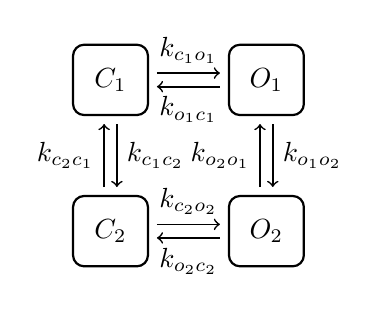
\begin{tikzpicture}[
   font=\sffamily,
   every matrix/.style={ampersand replacement=\&,column sep=1cm,row sep=1cm},
   state/.style={draw,thick,rounded corners,inner sep=.3cm},
   to/.style={->,semithick,shorten >=0.1cm,shorten <=0.1cm},
   Q/.style={->,semithick,sloped,pos=0.700000,shorten >=0.1cm,shorten <=0.1cm},  
   every node/.style={auto}]
\matrix{
\node[state] (C_{1}) {\parbox{10pt}{\centerline{$C_{1}$}}};\&\node[state] (O_{1}) {\parbox{10pt}{\centerline{$O_{1}$}}};\\
\node[state] (C_{2}) {\parbox{10pt}{\centerline{$C_{2}$}}};\&\node[state] (O_{2}) {\parbox{10pt}{\centerline{$O_{2}$}}};\\
};
\draw[to]  (C_{1}.10) to node {$k_{c_{1}o_{1}}$} (O_{1}.170);
\draw[to]  (C_{1}.280) to node {$k_{c_{1}c_{2}}$} (C_{2}.80);
\draw[to]  (O_{1}.190) to node {$k_{o_{1}c_{1}}$} (C_{1}.350);
\draw[to]  (O_{1}.280) to node {$k_{o_{1}o_{2}}$} (O_{2}.80);
\draw[to]  (C_{2}.100) to node {$k_{c_{2}c_{1}}$} (C_{1}.260);
\draw[to]  (C_{2}.10) to node {$k_{c_{2}o_{2}}$} (O_{2}.170);
\draw[to]  (O_{2}.100) to node {$k_{o_{2}o_{1}}$} (O_{1}.260);
\draw[to]  (O_{2}.190) to node {$k_{o_{2}c_{2}}$} (C_{2}.350);
\end{tikzpicture}
\end{center}
\caption{Markov model including four possible states: two open states, $O_{1}$ 
and $O_{2}$, and two closed states, $C_{1}$ and $C_{2}$.}%
\label{M44}%
\end{figure}

The probability density system associated with the model $(\ref{c1g})$ and $(\ref{c2g})$ when the Markov model is given by Figure \ref{M44} can now be 
written in the form%

\begin{align}
\frac{\partial\rho_{o_{1}}}{\partial t}+\frac{\partial}{\partial x}\left(
a_{o}^{x}\rho_{o_{1}}\right)  +\frac{\partial}{\partial y}\left(  a_{o}%
^{y}\rho_{o_{1}}\right)   &  =k_{c_{1}o_{1}}\rho_{c_{1}}-\left(  k_{o_{1}%
c_{1}}+k_{o_{1}o_{2}}\right)  \rho_{o_{1}}+k_{o_{2}o_{1}}\rho_{o_{2}%
},\nonumber\\
\frac{\partial\rho_{o_{2}}}{\partial t}+\frac{\partial}{\partial x}\left(
a_{o}^{x}\rho_{o_{2}}\right)  +\frac{\partial}{\partial y}\left(  a_{o}%
^{y}\rho_{o_{2}}\right)   &  =k_{c_{2}o_{2}}\rho_{c_{2}}-\left(  k_{o_{2}c_{2}%
}+k_{o_{2}o_{1}}\right)  \rho_{o_{2}}+k_{o_{1}o_{2}}\rho_{o_{1}}%
,\label{pdf44}\\
\frac{\partial\rho_{c_{1}}}{\partial t}+\frac{\partial}{\partial x}\left(
a_{c}^{x}\rho_{c_{1}}\right)  +\frac{\partial}{\partial y}\left(  a_{c}%
^{y}\rho_{c_{1}}\right)   &  =k_{o_{1}c_{1}}\rho_{o_{1}}-\left(  k_{c_{1}%
o_{1}}+k_{c_{1}c_{2}}\right)  \rho_{c_{1}}+k_{c_{2}c_{1}}\rho_{c_{2}%
},\nonumber\\
\frac{\partial\rho_{c_{2}}}{\partial t}+\frac{\partial}{\partial x}\left(
a_{c}^{x}\rho_{c_{2}}\right)  +\frac{\partial}{\partial y}\left(  a_{c}%
^{y}\rho_{c_{2}}\right)   &  =k_{c_{1}c_{2}}\rho_{c_{1}}-\left(  k_{c_{2}%
c_{1}}+k_{c_{2}o_{2}}\right)  \rho_{c_{2}}+k_{o_{2}c_{2}}\rho_{o_{2}%
},\nonumber
\end{align}
where %
\begin{align}
a_{o}^{x} &  =v_{r}\left(  y-x\right)  +v_{d}\left(  c_{0}-x\right)
,\nonumber\\
a_{o}^{y} &  =v_{r}\left(  x-y\right)  +v_{s}\left(  c_{1}-y\right)
,\label{flux44}\\
a_{c}^{x} &  =v_{d}\left(  c_{0}-x\right)  ,\nonumber\\
a_{c}^{y} &  =v_{s}\left(  c_{1}-y\right)  .\nonumber
\end{align}
By defining the states $O_{1},O_{2},C_{1},$ and $C_{2}$ to be the states 
1, 2, 3, and
4, respectively, we can write the system $(\ref{pdf44})$ in the more compact form%
\begin{equation}
\frac{\partial\rho_{i}}{\partial t}+\frac{\partial}{\partial x}\left(
a_{i}^{x}\rho_{i}\right)  +\frac{\partial}{\partial y}\left(  a_{i}^{y}%
\rho_{i}\right)  =\left(  K\rho\right)  _{i}\label{compact44}%
\end{equation}
for $i=1,2,3,4,$ where%
\begin{align*}
a_{i}^{x} &  =\gamma_{i}v_{r}\left(  y-x\right)  +v_{d}\left(  c_{0}-x\right)
,\\
a_{i}^{y} &  =\gamma_{i}v_{r}\left(  x-y\right)  +v_{s}\left(  c_{1}-y\right),
\end{align*}
and $\rho=(\rho_1,\rho_2,\rho_3,\rho_4)^T.$ 
Here $\gamma_{i}$ is one for the open states (i.e., $i=1$ and $i=2$) and zero for
the closed states (i.e., $i=3$ and $i=4$). Furthermore, the matrix is given by%
\[
K=\left(
\begin{array}
[c]{cccc}%
-\left(  k_{o_{1}c_{1}}+k_{o_{1}o_{2}}\right)   & k_{o_{2}o_{1}} &
k_{c_{1}o_{1}} & 0\\
k_{o_{1}o_{2}} & -\left(  k_{o_{2}c_{2}}+k_{o_{2}o_{1}}\right)   & 0 &
k_{c_{2}o_{2}}\\
k_{o_{1}c_{1}} & 0 & -\left(  k_{c_{1}o_{1}}+k_{c_{1}c_{2}}\right)   &
k_{c_{2}c_{1}}\\
0 & k_{o_{2}c_{2}} & k_{c_{1}c_{2}} & -\left(  k_{c_{2}c_{1}}+k_{c_{2}o_{2}%
}\right)
\end{array}
\right),
\]
which in compact notation is%
\[
K=\left(
\begin{array}
[c]{cccc}%
-\left(  k_{13}+k_{12}\right)   & k_{21} & k_{31} & 0\\
k_{12} & -\left(  k_{24}+k_{21}\right)   & 0 & k_{42}\\
k_{13} & 0 & -\left(  k_{31}+k_{34}\right)   & k_{43}\\
0 & k_{24} & k_{34} & -\left(  k_{43}+k_{42}\right)
\end{array}
\right)  .
\]

\bigskip
\section{Nine-state model}

We have seen how to formulate probability density systems for two-state and
four-state Markov models.  For even larger Markov models, it is useful to
introduce two-dimensional numbering. This will be illustrated using the nine-state model 
given in Figure \ref{ninestates}.%
\begin{figure}[ptb]
\begin{center}
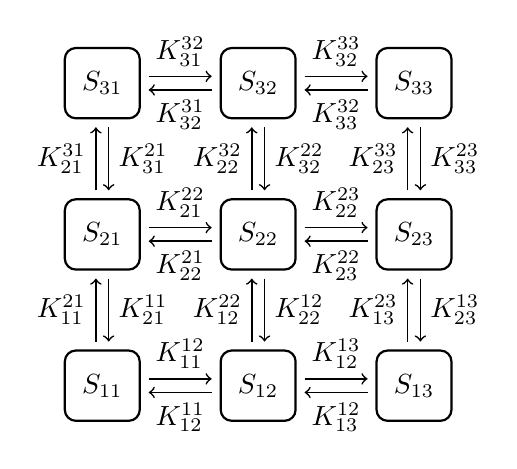
\begin{tikzpicture}[
   font=\sffamily,
   every matrix/.style={ampersand replacement=\&,column sep=1cm,row sep=1cm},
   state/.style={draw,thick,rounded corners,inner sep=.3cm},
   to/.style={->,semithick,shorten >=0.1cm,shorten <=0.1cm},
   Q/.style={->,semithick,sloped,pos=0.700000,shorten >=0.1cm,shorten <=0.1cm},  
   every node/.style={auto}]
\matrix{
\node[state] (S_{31}) {\parbox{10pt}{\centerline{$S_{31}$}}};\&\node[state] (S_{32}) {\parbox{10pt}{\centerline{$S_{32}$}}};\&\node[state] (S_{33}) {\parbox{10pt}{\centerline{$S_{33}$}}};\\
\node[state] (S_{21}) {\parbox{10pt}{\centerline{$S_{21}$}}};\&\node[state] (S_{22}) {\parbox{10pt}{\centerline{$S_{22}$}}};\&\node[state] (S_{23}) {\parbox{10pt}{\centerline{$S_{23}$}}};\\
\node[state] (S_{11}) {\parbox{10pt}{\centerline{$S_{11}$}}};\&\node[state] (S_{12}) {\parbox{10pt}{\centerline{$S_{12}$}}};\&\node[state] (S_{13}) {\parbox{10pt}{\centerline{$S_{13}$}}};\\
};
\draw[to]  (S_{31}.10) to node {$K_{31}^{32}$} (S_{32}.170);
\draw[to]  (S_{31}.280) to node {$K_{31}^{21}$} (S_{21}.80);
\draw[to]  (S_{32}.190) to node {$K_{32}^{31}$} (S_{31}.350);
\draw[to]  (S_{32}.10) to node {$K_{32}^{33}$} (S_{33}.170);
\draw[to]  (S_{32}.280) to node {$K_{32}^{22}$} (S_{22}.80);
\draw[to]  (S_{33}.190) to node {$K_{33}^{32}$} (S_{32}.350);
\draw[to]  (S_{33}.280) to node {$K_{33}^{23}$} (S_{23}.80);
\draw[to]  (S_{21}.100) to node {$K_{21}^{31}$} (S_{31}.260);
\draw[to]  (S_{21}.10) to node {$K_{21}^{22}$} (S_{22}.170);
\draw[to]  (S_{21}.280) to node {$K_{21}^{11}$} (S_{11}.80);
\draw[to]  (S_{22}.100) to node {$K_{22}^{32}$} (S_{32}.260);
\draw[to]  (S_{22}.190) to node {$K_{22}^{21}$} (S_{21}.350);
\draw[to]  (S_{22}.10) to node {$K_{22}^{23}$} (S_{23}.170);
\draw[to]  (S_{22}.280) to node {$K_{22}^{12}$} (S_{12}.80);
\draw[to]  (S_{23}.100) to node {$K_{23}^{33}$} (S_{33}.260);
\draw[to]  (S_{23}.190) to node {$K_{23}^{22}$} (S_{22}.350);
\draw[to]  (S_{23}.280) to node {$K_{23}^{13}$} (S_{13}.80);
\draw[to]  (S_{11}.100) to node {$K_{11}^{21}$} (S_{21}.260);
\draw[to]  (S_{11}.10) to node {$K_{11}^{12}$} (S_{12}.170);
\draw[to]  (S_{12}.100) to node {$K_{12}^{22}$} (S_{22}.260);
\draw[to]  (S_{12}.190) to node {$K_{12}^{11}$} (S_{11}.350);
\draw[to]  (S_{12}.10) to node {$K_{12}^{13}$} (S_{13}.170);
\draw[to]  (S_{13}.100) to node {$K_{13}^{23}$} (S_{23}.260);
\draw[to]  (S_{13}.190) to node {$K_{13}^{12}$} (S_{12}.350);
\end{tikzpicture}
\end{center}
\caption{Markov model including nine possible states.}%
\label{ninestates}%
\end{figure}
Here $S_{ij},$ $i,j=1,2,3$, denotes the states of the Markov model and
$K_{ij}^{mn}$ denotes\footnote{We use $K_{ij}$ as shorthand for $K_{i,j},$ but
we use the comma when an index of the form $j+1$ is needed, that is we write
$K_{i,j+1}.$} the reaction rate from the state $S_{ij}$ to the state $S_{mn}.$
The system governing the probability density functions of these states can be
written in the form%
\begin{equation}
\frac{\partial\rho_{ij}}{\partial t}+\frac{\partial}{\partial x}\left(
a_{ij}^{x}\rho_{ij}\right)  +\frac{\partial}{\partial y}\left(  a_{ij}^{y}%
\rho_{ij}\right)  =R_{ij},\label{pdf99}%
\end{equation}
where%
\begin{align*}
R_{ij}  & =K_{i,j+1}^{i,j}\rho_{i,j+1}+K_{i+1,j}^{i,j}\rho_{i+1,j}%
+K_{i,j-1}^{i,j}\rho_{i,j-1}+K_{i-1,j}^{i,j}\rho_{i-1,j}\\
& -\left(  K_{i,j}^{i,j+1}+K_{i,j}^{i+1,j}+K_{i,j}^{i,j-1}+K_{i,j}%
^{i-1,j}\right)  \rho_{i,j}.
\end{align*}
Here $\rho_{ij}$ denotes the probability density function of the state
$S_{ij}$ and we use the convention that $K_{ij}^{mn}=0$ for $i,j,m,n\notin%
\left\{  1,2,3\right\}  .$ We also have%
\begin{align*}
a_{ij}^{x} &  =\gamma_{ij}v_{r}\left(  y-x\right)  +v_{d}\left(
c_{0}-x\right)  ,\\
a_{ij}^{y} &  =\gamma_{ij}v_{r}\left(  x-y\right)  +v_{s}\left(
c_{1}-y\right)  ,
\end{align*}
where $\gamma_{ij}=1$ when the state $S_{ij}$ represents an open state and
$\gamma_{ij}=0$ when $S_{ij}$ represents a closed state.




\input{Ca_V_L/Ca_V}
\input{Ionchannels_L/Ionchannels}


\chapter{A simple model of the sodium channel}
\label{simple_Na}

In the previous two chapters, we studied a prototypical model of an ion
channel. The model consisted of a differential equation involving a gating
mechanism that could be either open or closed. A Markov model governed the
gating and we derived a system giving the probability density functions of
the states involved in the Markov model. We used the probability density
approach to compute optimal theoretical drugs and noted that a mutation
leading to an increase in the closed to open reaction rate could be completely
repaired by an optimal closed state drug.

Next, we extended the prototypical model to also include an inactivated state.
The inactivated state can also be affected by mutations and we studied the
particular case in which the rates from inactivated to open and from 
inactivated to closed were increased by a factor $\mu$ referred to as the 
mutation severity index. In this case, we observed that an optimal drug was 
represented by a blocker associated with the inactivated state. We were again
able to completely repair the effect of the mutation using the theoretical
 drug.

In this chapter, we shall move closer to realistic Markov models of sodium
channels. These models tend to be somewhat more intricate than the
prototypical model we have studied so far. Providing Markov models of the
sodium channels has been a very active field of research for decades and a
series of models are available. We have chosen to study models that seem to
capture the basic structure applied in many models but are manageable from a
mathematical point of view. We choose this approach for clarity of
presentation and not for its ability to represent specific data. It is,
hopefully, quite clear that the method we use to analyze the models is
applicable to many other models.

Mutations of the sodium channel can lead to impaired inactivation. This may
lead to leakage of the sodium current, which can again trigger arrhythmias.
Here we will consider a model of the $\Delta$KPQ mutation of the SCN5A gene.
This mutation may lead to an arrhythmogenic disorder referred to as the long-QT
syndrome, which can lead to sudden cardiac death in the worst case. There are
several models representing the effect of the $\Delta$KPQ mutation. 
One that is well known is
provided by Clancy and Rudy \cite{Clancy1999}. Their approach to model the
impaired inactivation is to introduce a burst mode in the model where no
inactivation state is available. We will consider two ways of modeling the
effect of the mutation.

 In the first approach, we will use the method
utilized above. We will simply increase the reaction rate from the inactivated
to the closed state and from the inactivated to the open state by a factor
$\mu\ge1$, referred to as the mutation severity index. This change will clearly
reduce the probability of being in the inactivated state. 
It is therefore a model of impaired inactivation.

The second approach is
to introduce a burst mode in the model. When the channel is in the burst mode,
there is no inactivated state. This model will be
parameterized such that it is highly unlikely that the channel will enter the
burst mode for the wild type case, but the probability of entering the burst
mode is considerably higher in the mutant case.

\section{Markov model of a wild type sodium channel}

Markov models have turned out to be a powerful tool in representing the physics
of the sodium channel and a series of alternatives have been proposed by
various authors. Since this is still a very active field of research, it is hard
to claim one particular model as the definitive model. We
shall therefore focus on a kind of model that has a structure that seems to
be more or less agreed upon but, as usual, we attack this problem with
simplicity in mind. This also holds true for the way we introduce the effect
of a mutation.

We start by considering a simple model of the sodium channel, illustrated in
Figure \ref{wtreac}. The actual functions used in our computations will be
given below. However, we should note that the functions will always be chosen
such that they satisfy the principle of detailed balance, which, for the model
given in Figure \ref{wtreac}, means that the following relation holds:
\begin{equation}
k_{io}k_{oc}k_{ci}=k_{oi}k_{ic}k_{co}. \label{db2}
\end{equation}
The model of the closed states deserves a comment or two. Let us assume that a
sodium channel consists of three subunits and these subunits may exist in two
states: closed or permissible. The whole channel is in the state $C_{0}$ if
all three units are in the permissible state. Over a brief period given
by $\Delta t$, the channel can change from the state $C_{0}$ to the open
state and the probability of this event is $\Delta t k_{co}$ or it can
change to the inactivated state with probability $\Delta t k_{ci}$. However, the
channel can also go from the permissible state $C_{0}$ to the state $C_{1}$ and 
the probability of doing this is $3\Delta t \beta$. The reason for the factor 
of three here is that it is sufficient that one of the three subunits closes. By
assuming that the subunits act independently, we find that the probability is
$3\Delta t \beta$. The same reasoning gives us the rest of the
transitions between the different closed states.

\begin{figure}[ptb]
\begin{center}
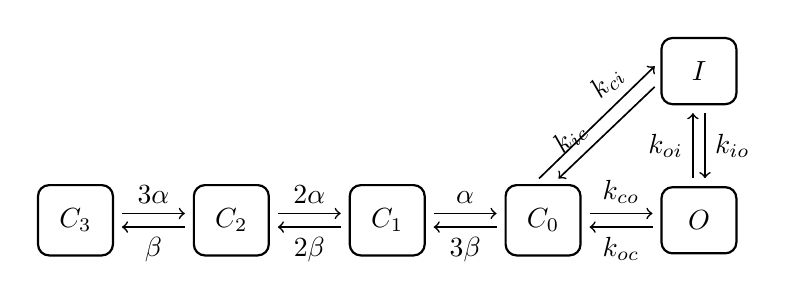
\begin{tikzpicture}[
   font=\sffamily,
   every matrix/.style={ampersand replacement=\&,column sep=1cm,row sep=1cm},
   state/.style={draw,thick,rounded corners,inner sep=.3cm},
   to/.style={->,semithick,shorten >=0.1cm,shorten <=0.1cm},
   Q/.style={->,semithick,sloped,pos=0.700000,shorten >=0.1cm,shorten <=0.1cm}, 
   every node/.style={auto}]
\matrix{
\&\&\&\&\node[state] (I) {\parbox{10pt}{\centerline{$I$}}};\\
\node[state] (C_{3}) {\parbox{10pt}{\centerline{$C_{3}$}}};\&\node[state] (C_{2}) {\parbox{10pt}{\centerline{$C_{2}$}}};\&\node[state] (C_{1}) {\parbox{10pt}{\centerline{$C_{1}$}}};\&\node[state] (C_{0}) {\parbox{10pt}{\centerline{$C_{0}$}}};\&\node[state] (O) {\parbox{10pt}{\centerline{$O$}}};\\
};
\draw[to]  (O.100) to node {$k_{oi}$} (I.260);
\draw[to]  (O.190) to node {$k_{oc}$} (C_{0}.350);
\draw[to]  (I.280) to node {$k_{io}$} (O.80);
\draw[Q]  (I.195) to node {$k_{ic}$} (C_{0}.75);
\draw[to]  (C_{0}.10) to node {$k_{co}$} (O.170);
\draw[Q]  (C_{0}.105) to node {$k_{ci}$} (I.165);
\draw[to]  (C_{0}.190) to node {$3\beta$} (C_{1}.350);
\draw[to]  (C_{1}.10) to node {$\alpha$} (C_{0}.170);
\draw[to]  (C_{1}.190) to node {$2\beta$} (C_{2}.350);
\draw[to]  (C_{2}.10) to node {$2\alpha$} (C_{1}.170);
\draw[to]  (C_{2}.190) to node {$\beta$} (C_{3}.350);
\draw[to]  (C_{3}.10) to node {$3\alpha$} (C_{2}.170);
\end{tikzpicture}
\end{center}
\caption{Markov model of a wild type sodium channel consisting of an open
state $(O)$, an inactivated state $(I)$, and four closed states $(C_{0}
,C_{1},C_{2},C_{3})$.}
\label{wtreac}
\end{figure}


\subsection{The equilibrium solution}

The equilibrium probabilities of the model given in Figure \ref{wtreac} are
characterized by the equations
\[
\begin{array}
[c]{ccc}
k_{ci}c_{0}=k_{ic}i, & k_{oi}o=k_{io}i, & k_{co}c_{0}=k_{oc}o,\\
3\beta c_{0}=\alpha c_{1}, & 2\alpha c_{2}=2\beta c_{1}, & 3\alpha c_{3}=\beta
c_{2},
\end{array}
\]
where $c_{0}$ denotes the equilibrium probability of being in the state
$C_{0}$. Similarly, the other variables are defined as the equilibrium
probability of being in the states $C_{1},C_{2},C_{3},I$, and $O$. We express all
probabilities in terms of the open probability:
\begin{align*}
i  &  =\frac{k_{oi}}{k_{io}}o,\text{ }c_{0}=\frac{k_{oc}}{k_{co}}o,\text{ }\\
c_{1}  &  =\frac{3\beta}{\alpha}\frac{k_{oc}}{k_{co}}o,\text{ }c_{2}
=\frac{3\beta^{2}}{\alpha^{2}}\frac{k_{oc}}{k_{co}}o,\text{ }c_{3}=\frac
{\beta^{3}}{\alpha^{3}}\frac{k_{oc}}{k_{co}}o.
\end{align*}
Since $o+i+c_{0}+c_{1}+c_{2}+c_{3}=1,$ we find the following equilibrium probabilities:

\begin{align}
o  &  =\frac{1}{q_{w}},\text{ }i=\frac{k_{oi}/k_{io}}{q_{w}},\text{ }
c_{0}=\frac{k_{oc}/k_{co}}{q_{w}}, \label{prob_wt}\\
c_{1}  &  =\frac{3\beta}{\alpha}\frac{k_{oc}/k_{co}}{q_{w}},\text{ }
c_{2}=\frac{3\beta^{2}}{\alpha^{2}}\frac{k_{oc}/k_{co}}{q_{w}},\text{ }
c_{3}=\frac{\beta^{3}}{\alpha^{3}}\frac{k_{oc}/k_{co}}{q_{w}},\nonumber
\end{align}
where
\[
q_{w}=1+\frac{k_{oi}}{k_{io}}+\frac{k_{oc}}{k_{co}}\left(  1+\beta
/\alpha\right)  ^{3}.
\]
Here the subscript $w$ is used to indicate that $q_{w}$ represents the 
wild type case.

\section{Modeling the effect of a mutation impairing the inactivated state}

The mutation impairs the inactivated state of the channel. In Section
\ref{mutaffectinactiv} we modeled this by increasing the probability of moving
from the inactivated state to the open state or to the closed state. This was
done by increasing the rates $k_{io}$ and $k_{ic}.$ We use the same approach
here and define
\begin{align}
\bar{k}_{ic}  &  =\mu k_{ic},\label{kic1}\\
\bar{k}_{io}  &  =\mu k_{io}, \label{kio2}
\end{align}
where, as usual, $\mu$ is the mutation severity index. From (\ref{db2}), we
have
\[
k_{io}k_{oc}k_{ci}=k_{ic}k_{co}k_{oi}
\]
and therefore
\[
\left(  \mu k_{io}\right)  k_{oc}k_{ci}=\left(  \mu k_{ic}\right)
k_{co}k_{oi};
\]
so
\[
\bar{k}_{io}k_{oc}k_{ci}=\bar{k}_{ic}k_{co}k_{oi}
\]
and thus the principle of detailed balance also holds for the mutant case,
in which the rates are given by $(\ref{kic1})$ and $(\ref{kio2}).$

\subsection{The equilibrium probabilities}
The reaction scheme of the mutant is illustrated in Figure \ref{mtreac}. In
the mutant case, the equilibrium probabilities are given by
\begin{align}
o  &  =\frac{1}{q_{m}},\text{ }i=\frac{k_{oi}/\left(  \mu k_{io}\right)
}{q_{m}},\text{ }c_{0}=\frac{k_{oc}/k_{co}}{q_{m}}, \\
c_{1}  &  =\frac{3\beta}{\alpha}\frac{k_{oc}/k_{co}}{q_{m}},\text{ }
c_{2}=\frac{3\beta^{2}}{\alpha^{2}}\frac{k_{oc}/k_{co}}{q_{m}},\text{ }
c_{3}=\frac{\beta^{3}}{\alpha^{3}}\frac{k_{oc}/k_{co}}{q_{m}}, \nonumber
\end{align}
where
\[
q_{m}=1+\frac{k_{oi}}{\mu k_{io}}+\frac{k_{oc}}{k_{co}}\left(  1+\beta
/\alpha\right)  ^{3}.
\]
For the equilibrium state it is worth observing that, since
\[
i=\frac{k_{oi}/k_{io}}{\frac{k_{oi}}{k_{io}}+\mu\left(  1+\frac{k_{oc}}
{k_{co}}\left(  1+\beta/\alpha\right)  ^{3}\right)  },
\]
the probability of being in the inactivated state is reduced when $\mu$ is
increased. Similarly, we observe that the associated open probability given
by
\[
o=\frac{1}{1+\frac{k_{oi}}{\mu k_{io}}+\frac{k_{oc}}{k_{co}}\left(
1+\beta/\alpha\right)  ^{3}}
\]
increases as $\mu$ increases. Although these calculations concern the 
equilibrium state, this is a pretty strong hint of an increased open 
probability in the dynamic case as well and an increased open probability is 
exactly the problem one observes when inactivation is impaired.

\begin{figure}[ptb]
\begin{center}
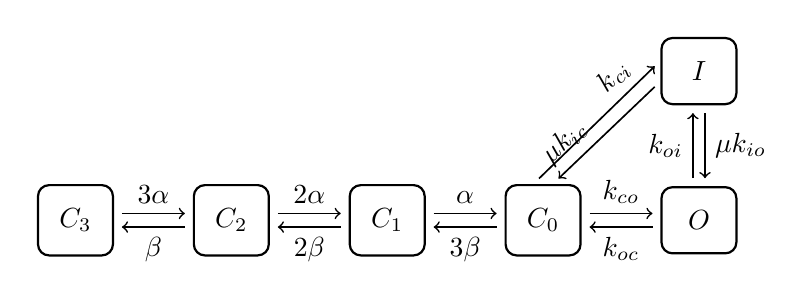
\begin{tikzpicture}[
   font=\sffamily,
   every matrix/.style={ampersand replacement=\&,column sep=1cm,row sep=1cm},
   state/.style={draw,thick,rounded corners,inner sep=.3cm},
   to/.style={->,semithick,shorten >=0.1cm,shorten <=0.1cm},
   Q/.style={->,semithick,sloped,pos=0.750000,shorten >=0.1cm,shorten <=0.1cm},  
   every node/.style={auto}]
\matrix{
\&\&\&\&\node[state] (I) {\parbox{10pt}{\centerline{$I$}}};\\
\node[state] (C_{3}) {\parbox{10pt}{\centerline{$C_{3}$}}};\&\node[state] (C_{2}) {\parbox{10pt}{\centerline{$C_{2}$}}};\&\node[state] (C_{1}) {\parbox{10pt}{\centerline{$C_{1}$}}};\&\node[state] (C_{0}) {\parbox{10pt}{\centerline{$C_{0}$}}};\&\node[state] (O) {\parbox{10pt}{\centerline{$O$}}};\\
};
\draw[to]  (O.100) to node {$k_{oi}$} (I.260);
\draw[to]  (O.190) to node {$k_{oc}$} (C_{0}.350);
\draw[to]  (I.280) to node {$\mu k_{io}$} (O.80);
\draw[Q]  (I.195) to node {$\mu k_{ic}$} (C_{0}.75);
\draw[to]  (C_{0}.10) to node {$k_{co}$} (O.170);
\draw[Q]  (C_{0}.105) to node {$k_{ci}$} (I.165);
\draw[to]  (C_{0}.190) to node {$3\beta$} (C_{1}.350);
\draw[to]  (C_{1}.10) to node {$\alpha$} (C_{0}.170);
\draw[to]  (C_{1}.190) to node {$2\beta$} (C_{2}.350);
\draw[to]  (C_{2}.10) to node {$2\alpha$} (C_{1}.170);
\draw[to]  (C_{2}.190) to node {$\beta$} (C_{3}.350);
\draw[to]  (C_{3}.10) to node {$3\alpha$} (C_{2}.170);
\end{tikzpicture}
\end{center}
\caption{Markov model of the mutant version of the sodium channel consisting of
an open state $(O)$, an inactivated state $(I)$, and four closed states
$(C_{0},C_{1},C_{2},C_{3})$. Here $\mu$ is referred to as the mutation
severity index.}
\label{mtreac}
\end{figure}

\bigskip


\section{Stochastic model of the sodium channel}




We use the same model of the transmembrane potential as above (see
(\ref{v1}) on page \pageref{v1}). Recall that the stochastic differential equation is
given by
\begin{equation}
Cv^{\prime}=-g_{L}\left(  v-V_{L}\right)  -\gamma g_{Na}(v-V_{Na}), \label{sv1}
\end{equation}
\graytable{l}{
{|c|c|} \hline
$C$ &  $1$ $\mu\text{F/cm}^{2}$\\ \hline
$g_L$ & $1/10 \text{ mS/cm}^{2}$ \\ \hline
$g_{Na}$ & $1\text{ mS/cm}^{2}$ \\ \hline
$V_L$ & $-85\text{ mV}$ \\ \hline
$V_{Na}$ & $45\text{ mV}$\\ \hline
}{Values of the parameters used in model \ref{sv1}.\label{scoef}}
where $C$ is the capacitance of the membrane, $V_{L}$ is the resting potential
of the leakage current, and $V_{Na}$ is the resting potential of the sodium
channel. The parameters are listed in Table \ref{scoef}.


%We use the following parameters:
%\begin{align}
%C  &  =1\mu\text{F/cm}^{2},\nonumber\\
%g_{L}  &  =\frac{1}{10}\text{mS/cm}^{2},\nonumber\\
%g_{Na}  &  =1\text{mS/cm}^{2}\label{scoef}\\
%V_{L}  &  =-85\text{mV,}\nonumber\\
%V_{Na}  &  =45\text{mV.}\nonumber
%\end{align}
The sodium channel can be either open (O), with $\gamma=1,$ or closed (C), with
$\gamma=0,$ and, as usual, the state of the channel is determined by a Markov
model. Since $C=1,$ we rewrite the equation in the more convenient form

\begin{equation}
v^{\prime}=-g_{L}\left(  v-V_{L}\right)  -\gamma g_{Na}(v-V_{Na}), \label{sv2}
\end{equation}
where $g_{L}$ and $g_{Na}$ now have the unit\footnote{The use of the odd units for 
$g_{L}$ and $g_{Na}$ stems from the fact that we have, for notational
 convenience, incorporated the capacitance of the membrane in these constants.}
$\text{ms}^{-1}.$

\subsection{A numerical scheme with an invariant region}

A numerical scheme for the model (ref{sv2}) can be written
in the form
\begin{equation}
v_{n+1}=v_{n}-\Delta t\left(  g_{L}\left(  v_{n}-V_{L}\right)  +\gamma
_{n}g_{Na}(v_{n}-V_{Na}\right)  ), \label{svs}
\end{equation}
where $\gamma_{n}$ is either zero or one and where $\Delta t$ denotes the
time step. We assume that the condition
\begin{equation}
\Delta t<\frac{1}{g_{L}+g_{Na}} \label{svdt}
\end{equation}
holds and, under this condition, we will show that an invariant region for the solutions
generated by the scheme (ref{svs}) is given by
\begin{equation}
\Omega=\left(  V_{L},V_{+}\right)  , \label{inv_region_2}
\end{equation}
where
\[
V_{+}=\frac{g_{L}V_{L}+g_{Na}V_{Na}}{g_{L}+g_{Na}}
\]
and, for the parameters we defined in (ref{scoef}), we have
$V_{+}\approx 33.18$ mV.
%\K{zzz xxxFor parametrene definert i (\ref{scoef}) f\r{a}r jeg 
%$V_{+}\approx 28.64$mV. Men dersom $V_{Na}=45$mV som det st\r{a}r i
%bildetekseten til Figure \ref{NaM:mc} stemmer det at $V_{+}\approx 33.18$mV.}\G{Har brukt  $V_{Na}=45$mV, endret til det i dokumentet}

To derive the invariant region, we proceed along the lines used on
page \pageref{vdt} and thus start by defining
\[
H(v,\gamma)=v-\Delta t\left(  g_{L}\left(  v-V_{L}\right)  +\gamma
g_{Na}(v-V_{Na}\right)  ).
\]
For values of $v$ in the region $\Omega$ and for values of $\Delta t$
satisfying condition (ref{svdt}), we have the properties
\[
\frac{d}{dv}H(v,\gamma)=1-\Delta t\left(  g_{L}+\gamma g_{Na}\right)
\geqslant1-\Delta t\left(  g_{L}+g_{Na}\right)  >0
\]
and
\[
\frac{d}{d\gamma}H(v,\gamma)=-\Delta t\left(  g_{Na}(v-V_{Na}\right)  )>0.
\]
Using these observations, we obtain
\[
v_{n+1}=H(v_{n},\gamma_{n})\leqslant H(V_{+},1)=V_{+}
\]
and
\[
v_{n+1}=H(v_{n},\gamma_{n})\geqslant H(V_{L},0)=V_{L}.
\]
So, by induction, it holds that $\Omega=\left(  V_{L},V_{+}\right)  $ is an
invariant region for scheme (ref{svs})


\section[Probability density functions]{Probability density functions for the
voltage-gated channel}
The systems modeling the probability density functions in the wild type 
and mutant cases are of exactly the same form; the only difference is
given by the mutation severity index. 
The probability density functions of the states of the Markov model given in
Figure \ref{mtreac} are given by
\begin{align}
\frac{\partial\rho_{o}}{\partial t}+\frac{\partial}{\partial v}\left(
a_{o}\rho_{o}\right)   &  =k_{co}\rho_{0}-\left(  k_{oc}+k_{oi}\right)
\rho_{o}+\mu k_{io}\rho_{i},\nonumber\\
\frac{\partial\rho_{i}}{\partial t}+\frac{\partial}{\partial v}\left(
a_{c}\rho_{i}\right)   &  =k_{oi}\rho_{o}-\mu\left(  k_{io}+k_{ic}\right)
\rho_{i}+k_{ci}\rho_{0},\nonumber\\
\frac{\partial\rho_{0}}{\partial t}+\frac{\partial}{\partial v}\left(
a_{c}\rho_{0}\right)   &  =k_{oc}\rho_{o}-\left(  k_{ci}+k_{co}+3\beta\right)
\rho_{0}+\mu k_{ic}i +\alpha \rho_{1} ,\label{vgpdf}\\
\frac{\partial\rho_{1}}{\partial t}+\frac{\partial}{\partial v}\left(
a_{c}\rho_{1}\right)   &  =2\alpha\rho_{2}-\left(  \alpha+2\beta\right)
\rho_{1}+3\beta\rho_{0},\nonumber\\
\frac{\partial\rho_{2}}{\partial t}+\frac{\partial}{\partial v}\left(
a_{c}\rho_{2}\right)   &  =3\alpha\rho_{3}-\left(  2\alpha+\beta\right)
\rho_{2}+2\beta\rho_{1},\nonumber\\
\frac{\partial\rho_{3}}{\partial t}+\frac{\partial}{\partial v}\left(
a_{c}\rho_{3}\right)   &  =-3\alpha\rho_{3}+\beta\rho_{2},\nonumber
\end{align}
where
\begin{align}
a_{o} &  =-g_{L}\left(  v-V_{L}\right)  -g_{Na}(v-V_{Na}),\label{sflux}\\
a_{c} &  =-g_{L}\left(  v-V_{L}\right)  ,\nonumber
\end{align}
with $\rho_{o}$ denoting the probability density function of being in the open
state, $\rho_{0}$ denoting the probability density function of being in the
state $C_{0},$ and so on.
%\K{zzz I de to f\o rste ligningene i dette systemet blir det brukt 
%$\rho_{c_{0}}$ i stedet for $\rho_{0}$. Er det noen grunn til det? 
%Dessuten ville jeg tro at man i tillegg til det som st\r{a}r der
%skulle legge til leddene 
%$+\alpha \rho_{1} - 3\beta \rho_{0}$ 
%p\r{a} h\o yresiden i den tredje ligningen. 
%Er det noen grunn til at man ikke gj\o r det?}
%\A{Both corrected: xxx  Glenn: make sure you correct the code accordingly.}
%\G{This was correct in the code.}

\subsection{Model parameterization}

To carry out numerical computations comparing the properties
of the  wild type and the mutant sodium channel, we need to define
the rates involved in the model described in Figure \ref{mtreac}. We use the 
rates
\[  k_{ab}(v) = k^{\infty}_{ab}(v)/\tau_{ab}, \ \ \  k_{ba}(v) = (1-k^{\infty}_{ab}(v))/\tau_{ab}, \]
with
\[k^{\infty}_{ab} = \frac{1}{1+e^{s_{a\!b}(V_{a\!b}-v)}}. \]
Furthermore, the rates $\alpha$ and $\beta$ in Figure \ref{mtreac} are given by
\[
\alpha =k^{\infty}_{cp}/\tau_{cp}  \text{ and } \beta =(1-k^{\infty}_{cp})/\tau_{cp}.
\]
With this parameterization, the principle of detailed balance is satisfied, provided that
\[ 
s_{co} + s_{ic} + s_{oi}=0 \mbox{\ \ and\ \ } s_{co}V_{co} + s_{oi}V_{oi} + s_{ic}V_{ic}  =0.  \]
The parameters are given in Table \ref{markov_rates} and we introduce the mutation as we
did in the previous chapter: We increase the probability of going from the
inactivated state to either the open or the closed state. More specifically, we define
\[
\bar{k}_{ic} = \mu k_{ic}  \text{ and } \bar{k}_{io} = \mu k_{io},
\] where, as usual, the wild type case is given by $\mu=1$. 

\begin{table}  \begin{center}
\begin{tabular}{|r|r|r|r|} \hline
$ab$ & $V_{ab}$ (mV) & $s_{ab}$ (1/mV) &  $\tau_{ab}$ (ms)\\ \hline
$co$ & -60 & 0.1& 0.01\\ \hline
$oi$ & -120 & 0.05 & 3 \\  \hline
$ic$ & -80 & -0.15& 10\\ \hline
$cp$ &-60 & 0.1& 0.1\\ \hline
\end{tabular} \end{center}
\caption{Parameters of the Markov model illustrated in Figures \ref{wtreac} 
and \ref{mtreac}. 
%\K{zzz Skal man oppgi enheter for disse parametrene?}
} 
\label{markov_rates} 
\end{table}

\subsection{Numerical experiments comparing the properties of the wild type 
and the mutant sodium channel}



In Figure \ref{NaM:pdf3}, we show the
probability density functions of the open state, the inactivated state, and the
sum of the closed states for the wild type case $(\mu=1)$ and two mutations
$(\mu=10$ and $\mu=30).$ The properties of the solutions are summarized in
Table \ref{na_stat}, which presents the expected values of the open state, the
inactivated state, and the sum of the closed states.


FIGURE: [fig/NaM_pdf3.pdf, width=500 frac=0.8] The probability density functions of the open state (left),
the sum of the closed states  (center), and the inactivated state (right) 
for the wild type case (solid line) and two values of the mutation severity 
index: $\mu=10$ and $\mu=30$. The strongest mutation differs the most
from the wild type solution. 
%{\bf xxx Glenn: something wrong here - read text and compare with headings of figures} \G{yes, fixed now.}
 label{NaM:pdf3}%\begin{table}  \begin{center}
%\begin{tabular}{|r|r|r|r|} \hline
%$\mu$ & $E_o$ & $E_i$ & $E_c$ \\ \hline
%1 & -50.8 & -84.9 & -83.5 \\ \hline
%10 & -13.4 & -84.9 & -57.0 \\ \hline
%30 & 13.0 & -84.9 & -20.8 \\ \hline
%\end{tabular} \end{center}
%\caption{Expected value of pdfs for WT and MT.
%{\bf xxx Glenn: Kan du legge inn $\pi_o,\pi_i,\pi_c$ i samme tabell?}}\label{na%_stat}
%\end{table}


%\begin{table}  \begin{center}
%\begin{tabular}{|r|r|r|r|r|r|r|} \hline
%$\mu$ & $\pi_o$ & $\pi_i$ & $\pi_c$ & $\rho_o$ & $\rho_i$ & $\rho_c$ \\ \hline
%1 & 0.0001 & 0.9951 & 0.0048 & -50.8 & -84.9 & -83.5 \\ \hline
%10 & 0.0002 & 0.9989 & 0.0009 & -13.4 & -84.9 & -57.0 \\ \hline
%30 & 0.0015 & 0.9941 & 0.0044 & 13.0 & -84.9 & -20.8 \\ \hline
%\end{tabular} \end{center}

\begin{table}  \begin{center}
\begin{tabular}{|r|r|r|r|r|r|r|} \hline
$\mu$ & $\pi_o\times 100 $ & $\pi_c$ & $\pi_i\times 100$ & $E_o$ & $E_c$ & $E_i$ \\ \hline
1 & 0.0067 & 0.9951 & 0.4834 & -50.8 & -84.9 & -83.5 \\ \hline
3 & 0.0080 & 0.9982 & 0.1765 & -41.1 & -84.9 & -79.6 \\ \hline
10 & 0.0162 & 0.9989 & 0.0942 & -13.4 & -84.9 & -57.0 \\ \hline
\end{tabular} \end{center}
\caption{Probability of being in the open, closed, or inactivated states and the expected value of the transmembrane
potential, provided that the channel is open, closed, or inactivated.}
%{\bf xxx Glenn xxx: Something wrong here since probability of being in inactivated state increases for increasing $\mu$.
%I guess it is ok that the channel almost certainly inactivate but that should be less likely when $\mu$ increases.
%Since numbers are small: refine mesh and refine stopping criterions?}}
\label{na_stat}
\end{table}




\subsection{Stochastic simulations illustrating the late sodium current in the mutant case}


Impaired inactivation of the sodium channel leads to a late sodium current,
which is illustrated in Figure \ref{NaM:mc}. The figure also includes 
experimental data of the sodium current taken from Bennett et al. 
\cite{Bennett1995}. We observe that, by
using $\mu=30$, the model fits the experimental data fairly well.

%FIGURE: [fig/NaM_mc.pdf, width=500 frac=0.8] Current for $\mu=1,10,30,100$. label{NaM:mc}\begin{figure}[p]\centering
\vbox{
\includegraphics[width=0.9\linewidth]{NaM/mc.pdf}
\includegraphics[width=0.7\linewidth]{NaM/Bennet.png}
}
\caption{Currents computed using the Markov model given in Figure \ref{mtreac}. Top panel: Currents based on numerical simulations for  $\mu=1,10,30,100$. Each trace is an average of 10,000 Monte Carlo runs. The current is given by $I=g_{Na} P_o (v-V_{Na})$, with the transmembrane potential clamped at $v=0$. The currents are normalized so that the wild type case peaks at -1. The parameters are given by $V_{Na} = 45$ and $g_{Na} = 1$ and $P_o$ is the average ratio of open channels over 10,000 runs, computed at each time step. The lower graphs are from Bennett et al. \cite{Bennett1995}, for the wild type case (left) and mutant case (right). 
%\K{zzz Skal man ha med enheter her?} 
\label{NaM:mc} }
%\K{zzz Hva st\r{a}r $P_{o}$ for?}}
%\A{xxx Glenn; check that the definition $P_o$ adheres with the one you have used in code.}
%\G{$P_o$: Ratio of open channels, taken over 10000 runs.}
\end{figure}

\section[Theoretical drug for the Sodium channel]{A theoretical drug repairing the sodium channel mutation}

We introduce a theoretical drug for the sodium channel of the form given in
Figure \ref{mtreadr}. The equilibrium probabilities of the model are characterized by the equations
\[
\begin{array}
[c]{ccc}
k_{ci}c_{0}=\mu k_{ic}i, & k_{oi}o=\mu k_{io}i, & k_{co}c_{0}=k_{oc}o,\\
3\beta c_{0}=\alpha c_{1}, & 2\alpha c_{2}=2\beta c_{1}, & 3\alpha c_{3}=\beta
c_{2},\\
k_{bc}b_{0}=k_{cb}c_{0}, & k_{bc}b_{1}=k_{cb}c_{1}, & k_{bc}b_{2}=k_{cb}c_{2},\\
k_{bc}b_{3}=k_{cb}c_{3}, & k_{bi}b_{i}=k_{ib}i, & k_{bo}b_{o}=k_{ob}o.
\end{array}
\]
As usual, we express all probabilities in terms of the open state probability, \label{9001}
\begin{align*}
i &  =\frac{k_{oi}}{\mu k_{io}}o,\text{ }c_{0}=\frac{k_{oc}}{k_{co}}o,\text{
}\\
c_{1} &  =\frac{3\beta}{\alpha}\frac{k_{oc}}{k_{co}}o,\text{ }c_{2}
=\frac{3\beta^{2}}{\alpha^{2}}\frac{k_{oc}}{k_{co}}o,\text{ }c_{3}=\frac
{\beta^{3}}{\alpha^{3}}\frac{k_{oc}}{k_{co}}o,\\
b_{0} &  =\text{ }\delta_{c}\frac{k_{oc}}{k_{co}}o,\text{ }b_{1}=\text{
}\delta_{c}\frac{3\beta}{\alpha}\frac{k_{oc}}{k_{co}}o,\text{ }b_{2}=\text{
}\delta_{c}\frac{3\beta^{2}}{\alpha^{2}}\frac{k_{oc}}{k_{co}}o,\\
b_{3} &  =\text{ }\delta_{c}\frac{\beta^{3}}{\alpha^{3}}\frac{k_{oc}}{k_{co}
}o,\text{ }b_{i}=\delta_{i}\frac{k_{oi}}{\mu k_{io}}o,\text{ }b_{o}=\delta
_{o}o,
\end{align*}
where we have introduced the following parameters characterizing the drug:
\[
\delta_{o}=\frac{k_{ob}}{k_{bo}},\text{ }\delta_{i}=\frac{k_{ib}}{k_{bi}
},\text{ }\delta_{c}=\frac{k_{cb}}{k_{bc}}.
\]
Since the sum of the probabilities is one, we obtain
\[
o_{m,d}=\frac{1}{q_{m,d}},
\]
where the subscript indicates the mutant case in the presence of a drug. Here,
\[
q_{m,d}=1+\frac{k_{oi}}{\mu k_{io}}+\frac{k_{oc}}{k_{co}}\left(
1+\beta/\alpha\right)  ^{3}\left(  1+\delta_{c}\right)  +\delta_{i}
\frac{k_{oi}}{\mu k_{io}}+\delta_{o}
\]
and we recall that the wild type open probability is given by 
\[
o_{w}=\frac{1}{q_{w}},
\]
where
\[
q_{w}=1+\frac{k_{oi}}{k_{io}}+\frac{k_{oc}}{k_{co}}\left(  1+\beta
/\alpha\right)  ^{3}.
\]
Obviously, we obtain $o_{m,d}\approx o_{w}$, provided that $q_{m,d}\approx q_{w}$.
If we choose a drug characterized by
\begin{equation}
\delta_{o}=\delta_{c}=0,\text{and }\delta_{i}=\mu-1 \label{drg_inac}
\end{equation}
we find that
\[
q_{m,d}=1+\frac{k_{oi}}{k_{io}}+\frac{k_{oc}}{k_{co}}\left(  1+\beta
/\alpha\right)  ^{3}=q_{w}
\]
and therefore, with the drug specified by  $\left(  \ref{drg_inac}\right)
,$ we have $o_{m,d}=o_{w}$, so the open probability at equilibrium is repaired.



\begin{figure}[ptb]
\begin{center}
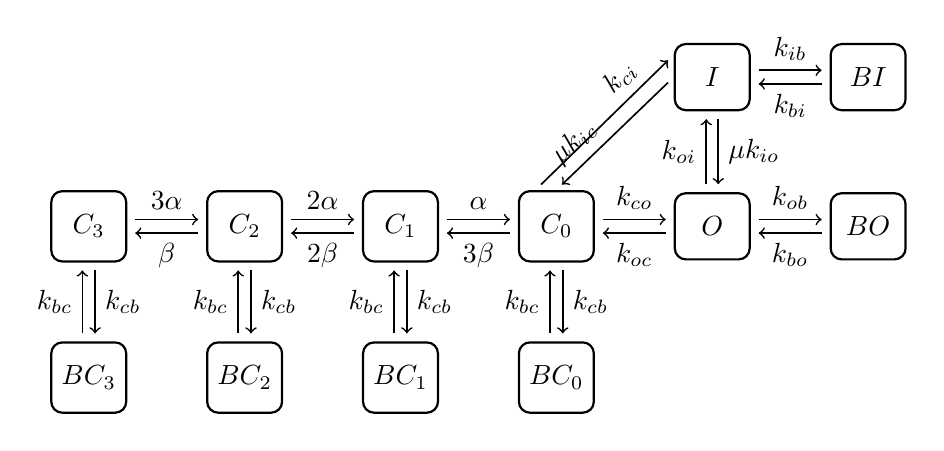
\begin{tikzpicture}[
   font=\sffamily,
   every matrix/.style={ampersand replacement=\&,column sep=1cm,row sep=1cm},
   state/.style={draw,thick,rounded corners,inner sep=.3cm},
   to/.style={->,semithick,shorten >=0.1cm,shorten <=0.1cm},
   Q/.style={->,semithick,sloped,below, above,pos=0.720000,shorten >=0.1cm,shorten <=0.1cm},  
   %Q/.style={->,semithick,pos=0.60000,shorten >=0.1cm,shorten <=0.1cm},  
   every node/.style={auto}]
\matrix{
\&\&\&\&\node[state] (I) {\parbox{10pt}{\centerline{$I$}}};\&\node[state] (BI) {\parbox{10pt}{\centerline{$BI$}}};\\
\node[state] (C_{3}) {\parbox{10pt}{\centerline{$C_{3}$}}};\&\node[state] (C_{2}) {\parbox{10pt}{\centerline{$C_{2}$}}};\&\node[state] (C_{1}) {\parbox{10pt}{\centerline{$C_{1}$}}};\&\node[state] (C_{0}) {\parbox{10pt}{\centerline{$C_{0}$}}};\&\node[state] (O) {\parbox{10pt}{\centerline{$O$}}};\&\node[state] (BO) {\parbox{10pt}{\centerline{$BO$}}};\\
\node[state] (BC_{3}) {\parbox{10pt}{\centerline{$BC_{3}$}}};\&\node[state] (BC_{2}) {\parbox{10pt}{\centerline{$BC_{2}$}}};\&\node[state] (BC_{1}) {\parbox{10pt}{\centerline{$BC_{1}$}}};\&\node[state] (BC_{0}) {\parbox{10pt}{\centerline{$BC_{0}$}}};\&\&\\
};
\draw[to]  (O.100) to node {$k_{oi}$} (I.260);
\draw[to]  (O.190) to node {$k_{oc}$} (C_{0}.350);
\draw[to]  (O.10) to node {$k_{ob}$} (BO.170);
\draw[to]  (I.280) to node {$\mu k_{io}$} (O.80);
\draw[Q]  (I.180) to node {$\mu k_{ic}$} (C_{0}.90);
\draw[Q]  (C_{0}.120) to node {$k_{ci}$} (I.150);
\draw[to]  (I.10) to node {$k_{ib}$} (BI.170);
\draw[to]  (C_{0}.10) to node {$k_{co}$} (O.170);
\draw[to]  (C_{0}.190) to node {$3\beta$} (C_{1}.350);
\draw[to]  (C_{0}.280) to node {$k_{cb}$} (BC_{0}.80);
\draw[to]  (C_{1}.10) to node {$\alpha$} (C_{0}.170);
\draw[to]  (C_{1}.190) to node {$2\beta$} (C_{2}.350);
\draw[to]  (C_{1}.280) to node {$k_{cb}$} (BC_{1}.80);
\draw[to]  (C_{2}.10) to node {$2\alpha$} (C_{1}.170);
\draw[to]  (C_{2}.190) to node {$\beta$} (C_{3}.350);
\draw[to]  (C_{2}.280) to node {$k_{cb}$} (BC_{2}.80);
\draw[to]  (C_{3}.10) to node {$3\alpha$} (C_{2}.170);
\draw[to]  (C_{3}.280) to node {$k_{cb}$} (BC_{3}.80);
\draw[to]  (BO.190) to node {$k_{bo}$} (O.350);
\draw[to]  (BI.190) to node {$k_{bi}$} (I.350);
\draw[to]  (BC_{0}.100) to node {$k_{bc}$} (C_{0}.260);
\draw[to]  (BC_{1}.100) to node {$k_{bc}$} (C_{1}.260);
\draw[to]  (BC_{2}.100) to node {$k_{bc}$} (C_{2}.260);
\draw[to]  (BC_{3}.100) to node {$k_{bc}$} (C_{3}.260);
\end{tikzpicture}
\end{center}
\caption{Markov model for a theoretical drug of the sodium channel. The model
consists of the usual states $O,I,C_{0},C_{1},C_{2}$, and $C_{3}$ and the blocked
states $BO,BI,BC_{0},BC_{1},BC_{2}$, and $BC_{3}$.}
\label{mtreadr}
\end{figure}




\subsection{Numerical experiments using the blocker of the inactivated state}

We have seen that a blocker of the inactivated state is a promising
candidate for repairing the mutation described in Figure \ref{mtreac}. The drug
is characterized by (ref{drg_inac}), so we have
\begin{equation}
k_{ib}=\delta_{i}k_{bi}=\left(  \mu-1\right)  k_{bi} \label{kbi10}
\end{equation}
and the parameter $k_{bi}$ remains to be determined. In Table \ref{kbi_stat}, we show that the
blocker is more efficient the larger $k_{bi}$ is. In fact, the blocker is able to
repair all the relevant statistical properties of the solution. The statistical properties
presented in the table are introduced in Section \ref{statistics} on page \pageref{statistics}.


In Figure \ref{NaM:pdf_drug}, we show the open state probability density functions of the
wild type, the mutant, and the drugged version of the mutant. Again, we see
that the drug completely repairs the open state probability density function.

FIGURE: [fig/NaM_pdf_drug.pdf, width=500 frac=0.8] The open probability density function for the wild type
(WT) case and the mutant (MT) case using the mutation severity index $\mu=30$
and, finally, the mutant case with the drug given by (\ref{kbi10}) with 
$k_{bi} = 0.001\text{ ms}^{-1}$. A small value of $k_{bi}$ was used to
see a difference between the drugged case and the WT case. label{NaM:pdf_drug}\begin{table}  \begin{center}
\begin{tabular}{|r|r|r|r|} \hline
$k_{bi}$ & $\pi_o\times 10^3 $ & $E_o$ & $\sigma_o$ \\ \hline
WT & 0.067 & -50.794 & 46.828 \\ \hline
MT & 1.534 & 12.991 & 26.831 \\ \hline
$10^{-6}$ & 1.341 & 12.940 & 26.913 \\ \hline
$10^{-5}$ & 1.180 & 12.487 & 27.634 \\ \hline
$10^{-4}$ & 0.556 & 8.240 & 33.343 \\ \hline
$10^{-3}$ & 0.135 & -16.903 & 49.326 \\ \hline
0.01 & 0.070 & -47.563 & 48.205 \\ \hline
0.1 & 0.067 & -50.729 & 46.869 \\ \hline
1 & 0.067 & -50.791 & 46.830 \\ \hline
\end{tabular} \end{center}
\caption{The open probability, $\pi_o$, the expected value of the transmembrane potential, $E_o$, and the
standard deviation, $\sigma_o$, for increasing values of $k_{bi}$. For large values of $k_{bi}$, the statistical properties 
of the mutant are completely repaired by the drug. 
}
\label{kbi_stat}
\end{table}

\subsection{The late sodium current is removed by the inactivated state blocker}


In Figure \ref{NaM:mc} above, we demonstrated, using Monte Carlo simulations, that the
mutation under consideration leads to a significant late sodium current
comparable to the current observed in experiments. By using the drug described
in (ref{drg_inac}) with $k_{bi}=0.01 \text{ ms}^{-1},$ we see that the late
current more or less completely disappears (see Figure \ref{NaM/mc_drug}).

\fig{NaM/mc_drug}{The sodium current for the wild type (WT) and the mutant (MT)
with the mutation severity index $\mu=30$. The drug given by (\ref{kbi10}) with $k_{bi} = 0.01 \text{ ms}^{-1}$
almost completely removes the late sodium current.}


\section{Notes}

\begin{enumerate}
\item The basic structure of the Markov model in Figure \ref{wtreac} is taken 
from Patlak \cite{Patlak1991}, who discusses and evaluates several possible models in relation to experimental data.

\item Modeling the effects of a drug on the sodium channel is motivated by
the paper of Clancy et al. \cite{Clancy2007}.


\end{enumerate}








\chapter{Mutations affecting the mean open time \label{mot_chapter}}

In the simplest case of Markov models of the form
\begin{equation}
C\underset{k_{co}}{\overset{k_{oc}}{\leftrightarrows}}O, \label{mot_markov}%
\end{equation}
we have studied mutations leading to an increased open probability by increasing
the rate from closed (C) to open (O), given by $k_{co}$. We refer to these as 
CO-mutations and for such mutations we
have successfully derived closed state blockers represented as%
\begin{equation}
B\underset{k_{bc}}{\overset{k_{cb}}{\leftrightarrows}}C\underset{\mu
k_{co}}{\overset{k_{oc}}{\leftrightarrows}}O, \label{mot_cl}%
\end{equation}
where $\mu\geqslant1$ is the mutation severity index and $\mu=1$
represents the wild type. These blockers can completely repair the equilibrium
open probability of the mutant by adjusting the ``on rate'' divided by the
``off rate'' of the drug given by
\[
\delta_{c}=\frac{k_{cb}}{k_{bc}}
\]
(see, e.g., page \pageref{d_c}). The remaining degree of freedom can be found
using probability density systems and the resulting drugs have been proven to
work exceptionally well in theoretical computations.

There is, however, another way of modeling increased equilibrium open
probability. Rather than increasing the rate from C to O, we can reduce the
rate from O to C:%
\begin{equation}
C\underset{k_{co}}{\overset{k_{oc}/\mu}{\leftrightarrows}}O,
\end{equation}
where again $\mu\geqslant1$ is referred to as the mutation severity index. 
This type of mutation is referred to as an OC-mutation and the
equilibrium open probability for this Markov model is given by%
\[
o=\frac{1}{1+\frac{k_{oc}/\mu}{k_{co}}},%
\]
which clearly increases for increasing values of $\mu.$ Formally, we can carry out
the same math to devise a closed state drug that completely repairs the
equilibrium open probability of the mutant; however, when this drug is put into the
probability density system to determine the remaining degree of
freedom of the drug, we quickly observe that the task is impossible and the
theoretical drug does not provide significant improvement.

The core difficulty here is that a CO-mutation does not
change the mean open time of the channel. A closed state blocker is therefore
well suited because such a blocker does not affect the mean open time. 
However, for an OC-mutation,
an increased mean open time is part of the problem and a closed state blocker
is not the solution, simply because it cannot affect the mean open time. Rather, an open state blocker must be used.

In this chapter, we will explain the notion of mean open time and study
mutations that lead to an increased open probability \textit{and} an increased mean
open time. We will show that open state blockers are optimal for such mutations.

\section{The mean open time}

Let us briefly recall the interpretation of the Markov model
\[
C\underset{k_{co}}{\overset{k_{oc}}{\leftrightarrows}}O.
\]
This scheme means that if the channel is closed (C), the probability of
changing the state from closed to open (O) in a small time interval $\Delta t$ is
given by $k_{co}\Delta t.$ Clearly, this interpretation only holds for short
time intervals, since the probability cannot exceed one. Note also that if the
rate $k_{co}$ increases, this leads to an increased probability of moving from C
to O during the time step $\Delta t.$ Similarly, $k_{oc}\Delta t$ denotes the
probability of moving from the open state to the closed state in the time step
$\Delta t.$

Suppose that the channel is open at time $t=0.$ The probability that the
channel remains open after a short time step $\Delta t$ is given by%
\[
p_{1}=1-k_{oc}\Delta t.
\]
If we take another time step, the probability that the channel is still open
at time $t=2\Delta t$ is given by%
\[
p_{2}=p_{1}\left(  1-k_{oc}\Delta t\right)  =\left(  1-k_{oc}\Delta t\right)
^{2}%
\]
and so on. At time $t=n\Delta t,$ the probability of the channel still being
open is given by%
\[
p_{n}=\left(  1-k_{oc}\Delta t\right)  ^{n}.
\]
If we now introduce time given by%
\[
t=n\Delta t,
\]
we have%
\[
\left(  1-k_{oc}\Delta t\right)  ^{n}=\left(  1-k_{oc}\Delta t\right)
^{\frac{t}{\Delta t}}.%
\]
The probability of closing a channel that is in the open state during a
time step is given by $\Delta tk_{oc}$ and therefore the probability of
closing a channel that has remained open for $n$ time steps is given by%
\[
\Delta tk_{oc}\left(  1-k_{oc}\Delta t\right)  ^{\frac{t}{\Delta t}}.
\]
The expected open time is therefore given by%
\[
\sum_{n=1}^{\infty}n\Delta t\left(  1-k_{oc}\Delta t\right)  ^{\frac{t}{\Delta
t}}\Delta tk_{oc}.
\]
If we go to the limit of $\Delta t\rightarrow0$ in this expression, we find
that%
\[
\sum_{n=1}^{\infty}n\Delta t\left(  1-k_{oc}\Delta t\right)  ^{\frac{t}{\Delta
t}}\Delta tk_{oc}\overset{\Delta t\rightarrow0}{\longrightarrow}\int%
_{0}^{\infty}tk_{oc}e^{-k_{oc}t}dt=\frac{1}{k_{oc}}%
\]
and therefore we have found that the mean open time is given by%
\begin{equation}
\tau_{o}=\frac{1}{k_{oc}}. \label{tau_o}%
\end{equation}


\subsection{Mean open time for more than one open state\label{mot_many}}


We have seen that the mean open time for a Markov model of the form
\[
C\underset{k_{co}}{\overset{k_{oc}}{\leftrightarrows}}O
\]
is given by
\begin{equation}
\tau_{o}=\frac{1}{k_{oc}}. %
\end{equation}
It is straightforward to extend the argument above to see that, for a Markov
model of the form 
\[
C\underset{k_{co}}{\overset{k_{oc}}{\leftrightarrows}}O\underset{k_{ob}}{\overset{k_{bo}}{\leftrightarrows}}B,
\]
the mean open time is given by
\begin{equation}
\tau_{o}=\frac{1}{k_{oc}+k_{ob}}. %
\end{equation}
But what happens if there is more than one open state? This situation
will become relevant below, where we consider models including a burst mode.
The models contain at least two open states. To understand the mean
open time in the presence of more than one open state, we consider the
generic extension illustrated in Figure \ref{o2}.

%
\begin{figure}[ptb]
\begin{center}
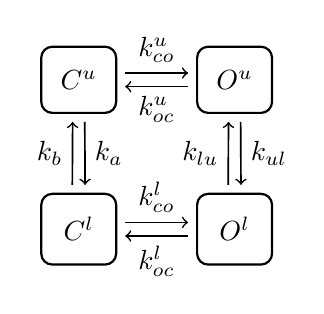
\begin{tikzpicture}[
   font=\sffamily,
   every matrix/.style={ampersand replacement=\&,column sep=1cm,row sep=1cm},
   state/.style={draw,thick,rounded corners,inner sep=.3cm},
   to/.style={->,semithick,shorten >=0.1cm,shorten <=0.1cm},
   Q/.style={->,semithick,sloped,pos=0.700000,shorten >=0.1cm,shorten <=0.1cm}, 
   every node/.style={auto}]
\matrix{
\node[state] (C^{u}) {\parbox{10pt}{\centerline{$C^{u}$}}};\&\node[state] (O^{u}) {\parbox{10pt}{\centerline{$O^{u}$}}};\\
\node[state] (C^{l}) {\parbox{10pt}{\centerline{$C^{l}$}}};\&\node[state] (O^{l}) {\parbox{10pt}{\centerline{$O^{l}$}}};\\
};
\draw[to]  (C^{u}.10) to node {$k_{co}^{u}$} (O^{u}.170);
\draw[to]  (C^{u}.280) to node {$k_{a}$} (C^{l}.80);
\draw[to]  (O^{u}.190) to node {$k_{oc}^{u}$} (C^{u}.350);
\draw[to]  (O^{u}.280) to node {$k_{ul}$} (O^{l}.80);
\draw[to]  (C^{l}.100) to node {$k_{b}$} (C^{u}.260);
\draw[to]  (C^{l}.10) to node {$k_{co}^{l}$} (O^{l}.170);
\draw[to]  (O^{l}.100) to node {$k_{lu}$} (O^{u}.260);
\draw[to]  (O^{l}.190) to node {$k_{oc}^{l}$} (C^{l}.350);
\end{tikzpicture}
\end{center}
\caption{Markov model with two open states ($O^{u}$, $O^{l}$) and two closed states ($C^{u}$, $C^{l}$).}%
\label{o2}%
\end{figure}
Assuming that the rates are set according to the principle of detailed balance,
 we have
\[k_{ul}o_{u}=k_{lu}o_{l}, \]
where $o_{u}$ and $o_{l}$ are the probabilities of being in the states 
$O^{u}$ or $O^{l}$, respectively, and $u$ and $l$ represent the upper and lower states,
respectively. 

As for the derivation above, we assume that the channel is open and
our task is to figure out how long we can expect the channel to remain open. We
know that, initially, the channel is either in the state $O^{u}$ or
$O^{l}$. Let us define $q_u$ and $q_l$ to be the conditional 
probabilities of being in the upper and lower open states, given that the channel is open. For the upper state we write
\[ q_u = P(S=O_u | (S={O_u} \mbox{\ or\ } S={O_l})), \]
where $S=X$ means that the channel is in state $X$.
Since
\[ P(A|B) = P(A \mbox{\ and\ } B)/P(B) \]
 and, in our case, since ($A$ and $B$) = $A$, we obtain
\[ q_u = P(S=O_u)/P(S={O_u} \mbox{\ or\ } S={O_l}) = \frac{o_u}{o_u+o_l} \]
and similarly for the lower state; with
\[ q_l = P(S=O_l | (S={O_u} \mbox{\ or\ } S={O_l})), \]
we obtain
\[ q_l  = \frac{o_l}{o_u+o_l}.\]
It follows that $q_u + q_l = 1$ and that

\[
q_{u}=\frac{k_{lu}}{k_{ul}+k_{lu}}%
\]
and%
\[
q_{l}=\frac{k_{ul}}{k_{ul}+k_{lu}}.
\]
The probability of remaining in the open states in the first time step is now given
by%
\begin{align*}
p_{1}  & =\left(  1-\Delta tk_{oc}^{u}\right)  q_{u}+\left(  1-\Delta
tk_{oc}^{l}\right)  q_{l}\\
& =1-\Delta t\left(  \frac{k_{oc}^{u}k_{lu}+k_{oc}^{l}k_{ul}}{k_{ul}+k_{lu}%
}\right)  
\end{align*}
and thus, by following the steps above, we find that%
\[
p_{n}=\left(  1-\Delta tK\right)  ^{n},
\]
where%
\[
K=\frac{k_{oc}^{u}k_{lu}+k_{oc}^{l}k_{ul}}{k_{ul}+k_{lu}}.
\]
The probability of closing a channel that is in one of the open states during
a time step is given by%
\[
\Delta tk_{oc}^{u}q_{u}+\Delta tk_{oc}^{l}q_{l}=\Delta tK
\]
and, therefore, the probability of closing a channel in a time step that has
remained open for $n$ time steps is given by%
\[
\Delta tK\left(  1-\Delta tK\right)^{n}.%
\]
We find  that the expected mean open time is given by%
\begin{equation}
\tau_{o}=\frac{1}{K}=\frac{k_{ul}+k_{lu}}{k_{oc}^{u}k_{lu}+k_{oc}^{l}k_{ul}}. \label{tau_oo}
\end{equation}

\subsubsection{Special cases}

It is interesting to consider the formula  for the mean open time given 
by $(\ref{tau_oo})$ in two special cases. First, we assume that 
$k^u_{oc}=k^l_{oc}$  and we let $k_{oc}$ denote this common value. Then, by $(\ref{tau_oo})$, we have 
\begin{equation*}
\tau_{o}=\frac{1}{k_{oc}}
\end{equation*}
which is the same as we found for the two-state scheme above. Next consider the case of $k_{ul}=k_{lu}$  (and 
$k^u_{oc}\not=k^l_{oc}$). By $(\ref{tau_oo})$, we find 
\begin{equation}
\tau_{o}=\frac{1}{(k_{oc}^{u}+k_{oc}^{u})/2}. \label{tau_ooo}
\end{equation}


\section{Numerical experiments}

It is useful to have a look at the mean open time computed in specific
numerical experiments to determine how well it is represented by the theoretical
value derived above. Similarly, it is useful to consider how well the
theoretical equilibrium open probability represents the data we observe in
actual computations. In this section, we will present experiments that
hopefully clarify these matters.

\subsection{Mean open time and equilibrium open probability: Theoretical
values versus sample mean values}

Let us illustrate the result above by a few numerical experiments. We start by
considering the Markov model%
\[
C\underset{k_{co}}{\overset{k_{oc}}{\leftrightarrows}}O,
\]
where we set $k_{co}=1$ ms$^{-1}$ and we let
\[
k_{oc}=\frac{1}{m}\text{ms}^{-1}%
\]
for $m=1,...,100.$ For every value of $k_{oc},$ we run a simulation using the
Markov model for $T=10^{4}$ ms. The time instances when the channel changes
state are stored in the sequence $\left\{  t_{i}\right\}  _{i=0}^{N}$ and the
mean open time observed in the simulation is given by\footnote{The
index $s$ here is used to indicate {\it sample}, since these are values for a
specific computation and not the theoretical value computed above.}
\[
\tau_{o,s}=\frac{2}{N}\sum_{i}\left(  t_{i}-t_{i-1}\right)  _{o},%
\]
where
\[
\left(  t_{i}-t_{i-1}\right)  _{o}=\left\{
\begin{array}
[c]{ll}%
t_{i}-t_{i-1}\text{ } & \text{if the channel is open in this interval,}\\
0\text{ } & \text{if the channel is closed in this interval.}%
\end{array}
\text{ }\right.
\]
With this notation we can also define the sample open probability by%
\[
o_{s}=\frac{1}{T}\sum_{i}\left(  t_{i}-t_{i-1}\right)  _{o}.
\]
In Figure  \ref{MOT/mot.pdf} (left panel), we plot the sample mean open time 
$\tau_{o,s}$ and the theoretical mean open time given by%
\begin{equation}
\tau_{o}=\frac{1}{k_{oc}} \label{mot2}%
\end{equation}
as functions of $k_{oc}.$ We also plot (right panel) the sample open
probability $o_{s}$ and the theoretical equilibrium probability given by%
\begin{equation}
o=\frac{1}{1+\frac{k_{oc}}{k_{co}}}. \label{mot3}%
\end{equation}
In both plots, we see that the mean values computed in the simulations are
quite close to the theoretical values. If we increase the simulation time $T,$
these graphs converge toward the same value.

\fig{MOT/mot.pdf}{Mean open time (left) and open probability (right), with $k_{oc}=1/m$ ms$^{-1}$ and $k_{co}=1$ ms$^{-1}$. The sample
values (dashed lines) correspond well with the theoretical values (solid line).}


\subsection{The closed to open rate $k_{co}$ does not affect the mean open
time}

We have seen that, theoretically, according to $\left(  \ref{mot2}\right)  ,$
the mean open time $\tau_{o}$ is independent of the closed to open rate
$k_{co},$ but the open probability is affected as stated in $\left(
\ref{mot3}\right)  .$ This is illustrated in Figure \ref{MOT/mct.pdf}, where we use
$k_{oc}=1$ ms$^{-1}$ and $k_{co}=1/m$ ms$^{-1}$ 
and plot the mean open time (left panel) and the open
probability (right panel) as functions of $m.$

\fig{MOT/mct.pdf}{Mean open time (left) and open probability (right) with $k_{co}=1/m$ ms$^{-1}$ and $k_{oc}=1$ ms$^{-1}$. The mean open
time is not affected by changes in $k_{co}$. The sample values correspond well to 
the theoretical values.}


\subsection{The mean open time in the presence of two open states}
In Figure \ref{MOT/burst_mot.pdf}, we show the sample mean open time and the theoretical mean open time given by 
\begin{equation}
\tau_{o}=\frac{1}{K}=\frac{k_{ul}+k_{lu}}{k_{oc}^{u}k_{lu}+k_{oc}^{l}k_{ul}} 
\end{equation}
for the Markov model in Figure \ref{o2}. In the computations, we have used $k^l_{oc} = 1$ ms$^{-1}$, $k^u_{oc} = 10$ ms$^{-1}$, and $k_{lu}  = 0.001$ ms$^{-1}$ and $k_{ul}$ varies. The other parameters of the model do not affect the result, as long as detailed balance holds.
\fig{MOT/burst_mot.pdf}{Mean open time for a Markov model with two open states.}


\subsection[Changing MOT affects the dynamics of the transmembrane potential]{Changing the mean open time affects the dynamics of the transmembrane potential}
%\K{zzz For meg virker det som at parametrene som i de tidligere kapitlene 
%har blitt kalt for $V_{Na}$ og lignende n\r{a} blir kalt for $E_{Na}$ og lignende.
%Hvis det er tilfellet, er det greit med to forskjellige notasjoner eller
%burde det brukes den samme notasjonen? I kapittel 12 ble de samme 
%parameterverdiene brukt, men da ble $g_{K}$ og $E_{K}$ kalt for $g_{L}$ og $V_{L}$.
%Er det meningen at dette skal v\ae re det samme eksempelet eller er dette et
%annet eksempel?}
%\A{I have changed all back to $V_{Na}$ and $V_{K}$.}
We consider the stochastic model of the transmembrane potential given by
\begin{equation}
v_{t}=g_{K}(V_{K}-v)+\gamma g_{Na}(V_{Na}-v) \label{mot_s_1},%
\end{equation}
where $\gamma$ is a stochastic variable governed by the two-state Markov
model
\[
C\underset{k_{co}}{\overset{k_{oc}}{\leftrightarrows}}O.
\]
We use the parameters%
\begin{align}
g_{K}  &  =\frac{1}{10}\text{ ms}^{-1},\text{ }g_{Na}=1\text{ ms}%
^{-1}, \label{mmm_dta}\\
V_{K} &  =-85\text{ mV, }V_{Na}=45\text{ mV,}\nonumber
\end{align}
and compute solutions using the standard scheme
\begin{equation}
v_{n+1}=v_{n}-\Delta t\left(  g_{K}\left(  v_{n}-V_{K}\right)  +\gamma
_{n}g_{Na}(v_{n}-V_{Na}\right)  ), \label{mot_vs}%
\end{equation}
where the time step is assumed to satisfy the condition%
\begin{equation}
\Delta t<\frac{1}{g_{K}+g_{Na}}.
\end{equation}
Under this condition, we have seen above that, for solutions computed by
$\left(  \ref{mot_s_1}\right),  $ an invariant region is given by
\begin{equation}
\Omega=\left(  V_{K},V_{+}\right)  ,
\end{equation}
where%
\[
V_{+}=\frac{g_{K}V_{K}+g_{Na}V_{Na}}{g_{K}+g_{Na}}.
\]
In Figure \ref{MOT/time.pdf}, we show numerical solutions of $\left(  \ref{mot_s_1}\right)  $
for
\[
k_{oc}=k_{co}=0.1\text{ ms}^{-1},1\text{ ms}^{-1}, 10\text{ ms}^{-1}, 100 \text{ ms}^{-1}.
\]
According to the considerations above, the equilibrium open probability is
given by%
\[
o=\frac{1}{1+\frac{k_{oc}}{k_{co}}},%
\]
which is constant for the four parameter sets used in Figure \ref{MOT/time.pdf}. The mean
open time, however, varies with $k_{oc}$ as%
\[
\tau_{o}=\frac{1}{k_{oc}}.
\]
For the cases studied in Figure \ref{MOT/time.pdf}, the mean open times are 
10 ms, 1 ms, 1/10 ms, and 1/100 ms and we observe that the reduced mean open time greatly 
reduces the variations of the transmembrane potential.

\fig[0.95]{MOT/time.pdf}{Simulations based on the numerical scheme (\ref{mot_vs}) with 
changing reaction rates for the Markov model.
From top to bottom, $k_{oc}=k_{co}=0.1\text{ ms}^{-1}$, $1 \text{ ms}^{-1}$, $10\text{ ms}^{-1}$, and $100 \text{ ms}^{-1}.$ 
Since $k_{oc}=k_{co}$ for all values, the open probability
is kept constant but the mean open time given by $1/k_{oc}$ is decreasing from top 
to bottom. }


\section[Changing MOT affects the PDFs]{Changing the mean open time affects the probability density functions}

The stationary version of the probability density system governing the states
of the Markov model%
\[
C\underset{k_{co}}{\overset{k_{oc}}{\leftrightarrows}}O
\]
is given by%

\begin{align}
\frac{\partial}{\partial v}\left(  a_{o}\rho_{o}\right)   &  =k_{co}\rho
_{c}-k_{oc}\rho_{o},\label{vpdf_mot}\\
\frac{\partial}{\partial v}\left(  a_{c}\rho_{c}\right)   &  =k_{oc}\rho
_{o}-k_{co}\rho_{c},\nonumber
\end{align}
where 
\begin{align}
a_{o}  &  =g_{K}(V_{K}-v)+g_{Na}(V_{Na}-v),\label{vflux_mot}\\
a_{c}  &  =g_{K}(V_{K}-v).\nonumber
\end{align}
The analytical solution of this problem is given by%

\begin{align*}
\rho_{o}(v)  &  =Kg_{K}(V_{+}-v)^{\frac{k_{oc}}{g}-1}(v-V_{K})^{\frac{k_{co}%
}{g_{K}}},\\
\rho_{c}(v)  &  =Kg(V_{+}-v)^{\frac{k_{oc}}{g}}(v-V_{K})^{\frac{k_{co}}{g_{K}}-1},%
\end{align*}
%\K{zzz Det skal vel egentlig st\r{a} v der det st\r{a}r x i disse uttrykkene?
%Og blir det ikke $(v-V_{K})$ i stedet for $(V_{K}-v)$ 
%siden vi antar $v \in (V_{K},V_{+})$?}\A{ Changed according to K.}
where
\[
g=g_{Na}+g_{K}\text{, }V_{+}=\frac{g_{Na}V_{Na}+g_{K}V_{K}}{g_{Na}+g_{K}}%
\]
%\K{zzz Denne E-en ble kalt for $V_{+}$ i forrige seksjon.}\A{ Changed according to K.}
and $K$ is chosen such that%
\[
\int_{V_{K}}^{V_{+}}\rho_{o}+\rho_{c}=1,
\]
which is given by
\[
1/K=\frac{k_{co}+k_{oc}}{a+b} (V_+-V_K)^{(a+b)} B(a,b),
\]
with $a = k_{co}/g_{K}, b = k_{oc}/g$, and $B(a,b) =\Gamma(a)\Gamma(b)/\Gamma(a+b)$.
%\K{zzz Burde det st\r{a} $V_{K}$ i stedet for $V_{-}$ i uttrykket slik at det henger mer sammen med det over?}


In Figure \ref{MOT/pdf.pdf}, we show the open probability density function for the data given
in $\left( \ref{mmm_dta}\right)  $ with
\[
k_{oc}=k_{co}=0.1 \text{ ms}^{-1},1\text{ ms}^{-1},10\text{ ms}^{-1},100 \text{ ms}^{-1}.
\]
Again, we recall that as $k_{oc}$ increases, the mean open time
decreases and we observe in the figure that the probability density function
becomes narrower.
%\K{zzz stoppet her}

\fig{MOT/pdf.pdf}{The open probability density function $\rho_o$ (solid line) and closed
 probability density function $\rho_c$ depend on the mean open time given by $1/k_{oc}$. In the figures,
 we have used $k=k_{oc}=k_{co}.$}

\bigskip

\begin{comment}
\subsection{The limit of the zero mean open time}

In Figure \ref{MOT/pdf.pdf}, we observed that as $k_{oc}$ and $k_{co}$ increase, the open
probability density function becomes increasingly narrow and it is tempting to
understand where this ends. Let $k=k_{oc}=k_{co}$ and consider the probability
density system%
\begin{align}
\frac{1}{k}\frac{\partial}{\partial v}\left(  a_{o}\rho_{o}\right)   &
=\rho_{c}-\rho_{o},\label{mot_k}\\
\frac{1}{k}\frac{\partial}{\partial v}\left(  a_{c}\rho_{c}\right)   &
=\rho_{o}-\rho_{c}.\nonumber
\end{align}
In the limit of $k\longrightarrow\infty,$ the mean open time
\[
\tau_{o}=\frac{1}{k_{oc}}=\frac{1}{k}\longrightarrow0
\]
and, by (\ref{mot_k}), we have
\[
\rho_{c}=\rho_{o}.
\]
By adding the equations, we obtain (for any value of $k$)%
\[
\frac{\partial}{\partial v}\left(  a_{o}\rho_{o}+a_{c}\rho_{c}\right)  =0
\]
and with $\rho_{o}=\rho_{c},$ this yields%
\[
\frac{\partial}{\partial v}\left(  \left(  a_{o}+a_{c}\right)  \rho
_{o}\right)  =0.
\]
Since $\rho_{o}=0$ for sufficiently large values of $\left\vert v\right\vert
,$ we find that%
\begin{equation}
\left(  a_{o}+a_{c}\right)  \rho_{o}=0 \label{0}%
\end{equation}
for almost all\footnote{This means {\sl almost all} in this sense: \url{http://en.wikipedia.org/wiki/Almost_all}.} $v$. Since
 $\rho_{o}=\rho_{c},$ we have%
\[
\int\rho_{o}dv=\frac{1}{2}%
\]
and thus $\rho_{o}=\frac{1}{2}\delta\left(  v-v_{\ast}\right)  , $ where
$\delta$ is the Dirac delta function. In general, we have%
\[
\int f(v)\delta\left(  v-v_{\ast}\right)  dv=f\left(  v_{\ast}\right)
\]
and, therefore, by (\ref{0}), we must have%
\[
\left(  a_{o}+a_{c}\right)  \left(  v_{\ast}\right)  =\frac{1}{2}\int\left(
a_{o}+a_{c}\right)  \left(  v\right)  \delta\left(  v-v_{\ast}\right)
dv=0.
\]
By using the definitions $\left(  \ref{vflux_mot}\right)  $, we obtain%
\[
2g_{K}(V_{K}-v_{\ast})+g_{Na}(V_{Na}-v_{\ast})=0
\]
and therefore%
\[
v_{\ast}=\frac{2g_{K}V_{K}+g_{Na}V_{Na}}{2g_{K}+g_{Na}}.
\]
In Figure \ref{MOT/pdf.pdf} we show the open and closed probability density functions
defined by the system $\left(  \ref{mot_k}\right)  .$ We observe that as $k$
increases, the functions converges and the distributions center around
$v_{\ast}=23.33$ mV. In these computations we have used the parameters defined in (\ref{mmm_dta}).

{\bf xxx Glenn: Kan du legge inn stoerre verdier av $k$ slik at vi ser at 
peak-verdier  konvergerer mot $v^*$?}
\G{Updated parameter value in text, peak should be at $v_{\ast}=23.33.$, so the plots are OK as is I guess.}

\end{comment}


\section{Theoretical drugs for OC-mutations}

We have seen earlier that when mutations increase the open probability by
increasing the reaction rate from C to O $(k_{co}),$ the effect of the
mutation can be completely repaired by using an optimal closed state blocker.
Now we are interested in a mutation that increases the open probability by reducing
the reaction rate from O to C $\left(  k_{oc}\right).$ Such a mutation
increases both the open probability and  the mean open time
and we will observe that a closed state blocker is unable to repair the effect
of such a mutation.

We consider the two-state Markov model
\begin{equation}
C\underset{k_{co}}{\overset{k_{oc}/\mu}{\leftrightarrows}}O, \label{mmm0}%
\end{equation}
where $\mu\geqslant1$ is the mutation severity index; as usual, $\mu=1$ denotes
the wild type. Recall that the equilibrium open probability is given by%
\[
o=\frac{1}{1+\frac{k_{oc}}{\mu k_{co}}}%
\]
and the mean open time is given by%
\[
\tau_{o}=\frac{\mu}{k_{oc}},%
\]
so the mutation clearly increases both the open probability and the mean open time.

\bigskip

\subsection{The theoretical closed state blocker does not work for the OC-mutation}

Let us start by considering a closed state blocker of the form%
\begin{equation}
B\underset{k_{bc}}{\overset{k_{cb}}{\leftrightarrows}}C\underset{k_{co}}{\overset{k_{oc}/\mu}{\leftrightarrows}}O. \label{mmm1}%
\end{equation}
%\K{zzz Burde man i denne Markov-modellen heller ta med at vi deler $k_{oc}$ 
%p\r{a} $\mu$?}
% A: ja; fixet
We find that the equilibrium open probability of the mutant in the presence of the
closed state blocker is given by%
\[
o=\frac{1}{1+\frac{k_{oc}}{k_{co}}\frac{1+\delta_{c}}{\mu}},%
\]
where%
\[
\delta_{c}=\frac{k_{cb}}{k_{bc}}.
\]
Since the wild type equilibrium open probability is given by%
\[
o=\frac{1}{1+\frac{k_{oc}}{k_{co}}},%
\]
the drug will repair the open probability, provided that%
\[
\frac{1+\delta_{c}}{\mu}=1
\]
and therefore the drug must satisfy the usual condition%
\[
\delta_{c}=\mu-1.
\]
A drug satisfying this condition will completely repair the equilibrium open
probability and that is, of course, good, but it is not enough. Since the
mutation represented by $\left(  \ref{mmm0}\right)  $ also affects the mean
open time, a drug of the form $\left(  \ref{mmm1}\right)  $ cannot repair that
effect of the mutation. To see this, we consider the probability
density system defined by%
\begin{align}
\frac{\partial}{\partial v}\left(  a_{o}\rho_{o}\right)   &  =k_{co}\rho
_{c}-\frac{1}{\mu}k_{oc}\rho_{o},\nonumber\\
\frac{\partial}{\partial v}\left(  a_{c}\rho_{c}\right)   &  =\frac{1}{\mu}k_{oc}\rho
_{o}-\left(  k_{co}+\left(  \mu-1\right)  k_{bc}\right)  \rho_{c}+k_{bc}%
\rho_{b},\label{mmm3}\\
\frac{\partial}{\partial v}\left(  a_{c}\rho_{b}\right)   &  =\left(
\mu-1\right)  k_{bc}\rho_{c}-k_{bc}\rho_{b},\nonumber
\end{align}
%\K{zzz Skal man ikke i disse ligningene dele $k_{oc}$ p\r{a} $\mu$?}
where, as usual, $\rho_{o},\rho_{c},$ and $\rho_{b}$ denote the probability
density functions of the open (O), closed (C), and blocked (B) states,
respectively, and where the fluxes are defined by $\left(  \ref{vflux_mot}%
\right)  $. In Figure \ref{MOT/cb.pdf}, we compare the open probability density computed by
solving the system $\left(  \ref{mmm3}\right)  $ with the open probability
density of the wild type. The wild type probability density functions are
given by%

\begin{align}
\frac{\partial}{\partial v}\left(  a_{o}\rho_{o}\right)   &  =k_{co}\rho
_{c}-k_{oc}\rho_{o},\label{mmm4}\\
\frac{\partial}{\partial v}\left(  a_{c}\rho_{c}\right)   &  =k_{oc}\rho
_{o}-k_{co}\rho_{c},\nonumber
\end{align}
and the probability density functions of the mutant case are given by
\begin{align}
\frac{\partial}{\partial v}\left(  a_{o}\rho_{o}\right)   &  =k_{co}\rho
_{c}-\frac{1}{\mu}k_{oc}\rho_{o},\label{mutant44}\\
\frac{\partial}{\partial v}\left(  a_{c}\rho_{c}\right)   &  =\frac{1}{\mu}k_{oc}\rho
_{o}-k_{co}\rho_{c}.\nonumber
\end{align}
In the computations we have used the parameters given by $\left(
\ref{mmm_dta}\right)  $ and the rates%
\[
k_{co}=1\text{ ms}^{-1} \text{ and }k_{oc}=1\text{ ms}^{-1}.
\]
We use three values of the rates $k_{bc}$ and we observe that no parameter is
able to repair the open state probability density function of the mutation. In
Figure \ref{MOT/norm.pdf}, we show the norm of the difference between the open probability
density defined by $\left(  \ref{mmm3}\right)  $ and $\left(  \ref{mmm4}%
\right)  .$ The norm is defined by $\left(  \ref{norm}\right)  $ on page
\pageref{norm} and we see that no version of the closed state blocker defined 
by $\left(  \ref{mmm1}\right)  $ is able to repair the effect of the mutations
given by $\left(  \ref{mmm0}\right)  .$

\fig{MOT/cb.pdf}{The solid line represents the wild type solution and the dashed line represents the mutant. Various closed state drugs are applied, but none are able to repair the effect of the mutation.}

\fig{MOT/norm.pdf}{The norm of the difference between the wild type solution and the mutant after the drug is applied. 
The norm is defined by $\left(  \ref{norm}\right)  $ on page \pageref{norm}. We see that no value of the drug parameter 
$k_{bc}$ for the closed state blocker is able to repair the effect of the mutation.
}


\subsection{The theoretical open state blocker repairs the effect of the OC-mutation}

Next, we consider an open state blocker for the mutation leading to both an
increased open probability and an increased mean open time. The theoretical open 
state blocker can be written in the form%
\begin{equation}
C\underset{k_{co}}{\overset{k_{oc}/\mu}{\leftrightarrows}}O\underset{k_{ob}%
}{\overset{k_{bo}}{\leftrightarrows}}B, \label{mmob1}%
\end{equation}
where the parameters $k_{bo}$ and $k_{ob}$ define the theoretical drug. For this
Markov model, the equilibrium open probability is given by%
\[
o_{\mu}=\frac{1}{1+\frac{k_{oc}}{\mu k_{co}}+\frac{k_{ob}}{k_{bo}}}%
\]
and the mean open time is given by%
\[
\tau_{o,\mu}=\frac{1}{\frac{1}{\mu}k_{oc}+k_{ob}}.
\]
Since the associated wild type values are%
\[
o=\frac{1}{1+\frac{k_{oc}}{k_{co}}}%
\]
and
\[
\tau_{o}=\frac{1}{k_{oc}},
\]
we want to define the drug such that%
\[
1+\frac{k_{oc}}{\mu k_{co}}+\frac{k_{ob}}{k_{bo}}=1+\frac{k_{oc}}{k_{co}}%
\]
and%
\[
\frac{1}{\mu}k_{oc}+k_{ob}=k_{oc}.
\]
To satisfy these two requirements, we find that the drug must be given by
\begin{equation} \label{mot_o_drg}
\begin{aligned}
k_{ob}  &  =\frac{\mu-1}{\mu}k_{oc},\\
k_{bo}  &  =k_{co}.
\end{aligned}
\end{equation}

\subsection{The theoretical open state blocker is optimal}
We will show analytically that the open state blocker defined by (\ref{mmob1}) where the parameters are given by
(\ref{mot_o_drg}) is an optimal drug, in the sense that the effect of the mutation is completely repaired.
We start by observing that the probability density system associated with the Markov model  (\ref{mmob1}) is given by
\begin{align}
\frac{\partial}{\partial v}\left(  a_{o}\rho_{o}\right)   &  =k_{co}\rho
_{c}-(\mu^{-1}k_{oc}+k_{ob})\rho_{o}+k_{bo}\rho_{b},\nonumber\\
\frac{\partial}{\partial v}\left(  a_{c}\rho_{c}\right)   &  =\mu^{-1}%
k_{oc}\rho_{o}-k_{co}\rho_{c},\label{mm_dr_3}\\
\frac{\partial}{\partial v}\left(  a_{c}\rho_{b}\right)   &  =k_{ob}\rho
_{o}-k_{bo}\rho_{b}.\nonumber
\end{align}
If we insert the drug given by $\left(  \ref{mot_o_drg}\right)  $, we obtain the
system
\begin{align}
\frac{\partial}{\partial v}\left(  a_{o}\rho_{o}\right)   &  =k_{co}\rho
_{c}-k_{oc}\rho_{o}+k_{co}\rho_{b},\nonumber\\
\frac{\partial}{\partial v}\left(  a_{c}\rho_{c}\right)   &  =\mu^{-1}%
k_{oc}\rho_{o}-k_{co}\rho_{c},\label{mm_dr_o2}\\
\frac{\partial}{\partial v}\left(  a_{c}\rho_{b}\right)   &  =\left(
1-\mu^{-1}\right)  k_{oc}\rho_{o}-k_{co}\rho_{b}.\nonumber
\end{align}
We define%
\[
\bar{\rho}_{c}=\rho_{c}+\rho_{b}%
\]
and add the two latter equations of this system to find that $\rho_{o}$ and 
$\bar{\rho}_{c}$ solve the system%
\begin{align}
\frac{\partial}{\partial v}\left(  a_{o}\rho_{o}\right)   &  =k_{co}\bar{\rho
}_{c}-k_{oc}\rho_{o},\\
\frac{\partial}{\partial v}\left(  a_{c}\bar{\rho}_{c}\right)   &  =k_{oc}%
\rho_{o}-k_{co}\bar{\rho}_{c},\nonumber
\end{align}
which coincides with the system defining the wild type probability density
functions (see $\left(  \ref{mmm4}\right)  $ above). We therefore conclude that
the open state blocker defined by the parameters 
$\left(  \ref{mot_o_drg}\right)  $
completely repairs the probability density functions of the mutant for any
value of the mutation severity index.

\bigskip

\subsubsection{The probability density function of the blocked state is
proportional to the probability density function of the wild type closed state}


In Figure \ref{MOT/ob.pdf}, we show the open probability density functions of the
wild type
(defined by system $\left(  \ref{mmm4}\right)  ),$ the mutant (defined by system $\left(  \ref{mutant44}\right)  $ with $\mu=3),$ 
%\K{zzz (\ref{mmm3}) er ligningene for closed state blocker. 
%Tror ikke at ligningene for mutant uten drug st\r{a}r noe sted.} 
and the mutant including the optimal drug (defined by system 
$\left(  \ref{mm_dr_o2} \right)  ).$ As expected, the open probability is 
completely repaired by the theoretical drug.

In the right panel of the figure, we show the graph of $\rho_{c}$ for the wild type
(solid line) and for the mutant case in the presence of the open blocker. We show
both $\rho_{c}$ and $\rho_{b}$. We note that these graphs seem to have the same 
shape  and we will show that they indeed differ only by a constant. 

We start by making the ansatz that for the solution of system $\left(  \ref{mm_dr_o2}\right)$ we have
\begin{equation}
\rho_{b}=\left(  \mu-1\right)  \rho_{c}. \label{mot_ans}%
\end{equation}
If we insert this into system $\left(  \ref{mm_dr_o2}\right)$, we find that
the two latter equations become identical and the system is therefore reduced to the following $2\times 2$
system:
\begin{align}
\frac{\partial}{\partial v}\left(  a_{o}\rho_{o}\right)   &  =\mu k_{co}%
\rho_{c}-k_{oc}\rho_{o},\nonumber\\
\frac{\partial}{\partial v}\left(  a_{c}\rho_{c}\right)   &  =\mu^{-1}%
k_{oc}\rho_{o}-k_{co}\rho_{c}.
\end{align}
Therefore, we can define
\[
\rho_{c}^{\ast}=\mu\rho_{c}%
\]
and find that $\rho_{o}$ and $\rho_{c}^{\ast}$ solve system%
\begin{align}
\frac{\partial}{\partial v}\left(  a_{o}\rho_{o}\right)   &  = k_{co}%
\rho_{c}^{\ast}-k_{oc}\rho_{o},\nonumber\\
\frac{\partial}{\partial v}\left(  a_{c}\rho_{c}^{\ast}\right)   &
=k_{oc}\rho_{o}-k_{co}\rho_{c}^{\ast},
\end{align}
which is exactly the wild type system. We therefore conclude that 
\begin{equation}
\rho_{b}=\left(  \mu-1\right)  \rho_{c}=\frac{\mu-1}{\mu}  \rho^*_{c}, \label{rb}
\end{equation}
where $(\rho_{o},\rho_{c},\rho_{b})$ solves the system $\left(  \ref{mm_dr_o2}\right)$
and where $(\rho^*_{o},\rho^*_{c})$ solves the wild type system
\begin{align*}
\frac{\partial}{\partial v}\left(  a_{o}\rho^*_{o}\right)   &  =k_{co}\rho^*_{c}-k_{oc}\rho^*_{o},\\
\frac{\partial}{\partial v}\left(  a_{c}\rho^*_{c}\right)   &  =k_{oc}%
\rho^*_{o}-k_{co}\rho^*_{c}.
\end{align*}

%{\bf Glenn: Can you check you numerical results and see if I have got the constant right; check the correctness
%of (\ref{rb}) by a numerical comparison.}
%\G{The ratios in Fig 13.9 are spot on (1/3 and 2/3).}
\fig{MOT/ob.pdf}{Probability density functions of the wild type, mutant, and mutant in the presence of the open blocker. The open blocker completely
repairs the open probability density function of the mutant. }


%\bf xxx Glenn: Is there something wrong in the right panel? In the
%left panel the two first curves are $\rho_o$ for wt and mt; but in the right panel it is
%$\rho_c$ for wt and

\subsection{Stochastic simulations using the optimal open state blocker}

In Figure \ref{MOT/ob_mc.pdf}, we show the results of numerical
simulations using scheme
$\left(  \ref{mot_vs}\right)  .$ We show the result for the wild type model
(upper panel), the mutant model (middle panel), and the model of the mutant 
where the drug defined by $\left(  \ref{mot_o_drg}\right)  $ is used (lower panel).

The graphs show that the effect of the mutation is repaired using the drug $\left(
\ref{mot_o_drg}\right) $; the solutions are not identical and this is
reasonable, since a random number generator is involved in updating the state
of the Markov model and therefore two computed solutions will not be identical
(not even two wild type solutions). However, we note that the qualitative properties
of the upper and lower solutions are similar, whereas the mutant case is
different due to the increased open probability and prolonged mean open time.

\fig{MOT/ob_mc.pdf}{Numerical simulations using scheme $\left(  \ref{mot_vs}\right) $
for wild type data (upper panel), mutant data (center panel), and mutant data where the drug
defined by $\left(  \ref{mot_o_drg}\right)$ is used (lower panel). 
Observe the long open periods in the middle panel
and that these are repaired by the drug (lower panel).}

\section{Inactivated states and mean open time}

In Chapter \ref{inactivated}, we studied a Markov model including the
open state (O), closed state (C), and inactivated state (I). The prototypical 
Markov model is repeated in Figure \ref{MOT_mut_L/ICO.pdf}.
 As usual, we assumed that the principle of detailed balance holds and
therefore the parameters of the Markov model satisfy the equation%
\begin{equation}
k_{io}k_{oc}k_{ci}=k_{oi}k_{co}k_{ic}.\label{db_m}%
\end{equation}
We also introduced a mutation that increased the rates $k_{io}$ and $k_{ic}$ and thus
reduced the probability of being in the inactivated state. From what we have
just seen, we readily observe that such a mutation does not influence the mean
open time; however, if data show that the mean open time is affected, the effect of
the mutation must be modeled differently. Another way to model the reduced
equilibrium probability of being in the inactivated state is to reduce the
rates toward the inactivated state. Such a mutation takes the form%
\begin{align}
\bar{k}_{ci} &  =k_{ci}/\mu,\label{ratesvm_m}\\
\bar{k}_{oi} &  =k_{oi}/\mu, \nonumber
\end{align}
where $\mu\geqslant1$ and, as usual, $\mu=1$ represents the wild type. It
follows from $\left(  \ref{db_m}\right)  $ that the principle of detailed
balance also holds for the mutant model:%
\begin{equation}
k_{io}k_{oc}\frac{k_{ci}}{\mu}=\frac{k_{oi}}{\mu}k_{co}k_{ic}.\label{db_mm}%
\end{equation}
If we repeat the argument above, we find that the mean open time of the model
presented in Figure \ref{MOT_mut_L/ICO.pdf} is given by%
\[
\tau_{o}=\frac{1}{k_{oc}+k_{oi}}% 
\]
for wild type data and
\[
\tau_{o,\mu}=\frac{1}{k_{oc}+k_{oi}/\mu}%
\]
for the mutant case. We note that the mean open time increases as the mutation severity
index $\mu$ increases. Following the usual steps, we find that the equilibrium
probabilities are given by
\begin{align*}
o &  =\frac{1}{1+\frac{k_{oc}}{k_{co}}+\frac{k_{oi}}{\mu k_{io}}},\\
c &  =\frac{\frac{k_{oc}}{k_{co}}}{1+\frac{k_{oc}}{k_{co}}+\frac{k_{oi}}{\mu
k_{io}}},\\
i &  =\frac{\frac{k_{oi}}{k_{io}}}{\mu\left(  1+\frac{k_{oc}}{k_{co}}\right)
+\frac{k_{oi}}{k_{io}}}.
\end{align*}
We observe that the equilibrium probability of being in the open and closed states
increases as a consequence of the mutation and the equilibrium probability of
being in the inactivated state is reduced under the mutation.

\begin{figure}[ptb]
\begin{center}
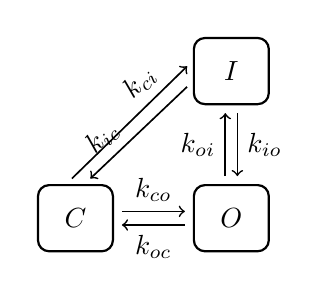
\begin{tikzpicture}[
   font=\sffamily,
   every matrix/.style={ampersand replacement=\&,column sep=1cm,row sep=1cm},
   state/.style={draw,thick,rounded corners,inner sep=.3cm},
   to/.style={->,semithick,shorten >=0.1cm,shorten <=0.1cm},
   Q/.style={->,semithick,sloped,pos=0.700000,shorten >=0.1cm,shorten <=0.1cm}, 
   every node/.style={auto}]
\matrix{
\&\node[state] (I) {\parbox{10pt}{\centerline{$I$}}};\\
\node[state] (C) {\parbox{10pt}{\centerline{$C$}}};\&\node[state] (O) {\parbox{10pt}{\centerline{$O$}}};\\
};
\draw[to]  (O.100) to node {$k_{oi}$} (I.260);
\draw[to]  (O.190) to node {$k_{oc}$} (C.350);
\draw[to]  (I.280) to node {$k_{io}$} (O.80);
\draw[Q]  (I.195) to node {$k_{ic}$} (C.75);
\draw[to]  (C.10) to node {$k_{co}$} (O.170);
\draw[Q]  (C.105) to node {$k_{ci}$} (I.165);
\end{tikzpicture}
\end{center}
\caption{Three-state Markov model. In the mutant case, we
replace the rates $k_{ci}$ and $k_{oi}$ by  $k_{ci}/\mu$ and $k_{oi}/\mu$, 
respectively, where $\mu$ denotes the mutation severity index.}
\label{MOT_mut_L/ICO.pdf}%
\end{figure}


%\fig[0.5]{MOT_mut_L/ICO.pdf}{Three state Markov model. In the mutant case we
%replace the rates $k_{ci}$ and $k_{oi}$ by  $k_{ci}/\mu$ and $k_{oi}/\mu$ where
%$\mu$ denotes the mutation severity index.}



\subsection{A theoretical open state blocker}



We observed above that to repair the effect of changes in the mean
open time, it is necessary to use an open state blocker. The reason for this is 
that neither a closed blocker nor an inactivated blocker has any effect on the 
mean open time and, therefore, it is inconceivable that such blockers 
can repair the effect of a mutation on the mean open time. An open state blocker 
directly affects the mean open time and the drug must be tuned to repair the 
effect of the mutation.

A Markov model that includes an open state blocker is shown in 
Figure \ref{MOT_mut_L/BICO_O.pdf}.
We have already computed
formulas for the equilibrium probabilities of a Markov model of this form (see
page \pageref{Ionchannels_L/BICO.pdf}). The inverse $(p=1/o)$ open probability in equilibrium is given by
\[
p_{\mu}=1+\frac{k_{oc}}{k_{co}}+\frac{1}{\mu}\frac{k_{oi}}{k_{io}}%
\]
and thus the wild type inverse open probability is given by%
\[
p=1+\frac{k_{oc}}{k_{co}}+\frac{k_{oi}}{k_{io}}.
\]
Similarly, the inverse open probability in the presence of the open state blocker 
is given by%
\[
p_{b,\mu}=1+\frac{k_{oc}}{k_{co}}+\frac{1}{\mu}\frac{k_{oi}}{k_{io}}+\frac{k_{ob}%
}{k_{bo}}.
\]
Furthermore, the mean open time of wild type is given by%
\[
\tau_{o}=\frac{1}{k_{oi}+k_{oc}}%
\]
and, when the theoretical drug is included in the mutant case, the mean open
time is given by%
\[
\tau_{o,b,\mu}=\frac{1}{\frac{1}{\mu}k_{oi}+k_{oc}+k_{ob}}.
\]
We are now looking for a drug that will repair the equilibrium probability and
the mean open time. More precisely, we want to find the parameters $k_{bo}$
and $k_{ob}$ such that $p_{b,\mu}=p$ and $\tau_{o,b,\mu}=\tau_{o}$. More explicitly, we require that
\[
1+\frac{k_{oc}}{k_{co}}+\frac{1}{\mu}\frac{k_{oi}}{k_{io}}+\frac{k_{ob}%
}{k_{bo}}=1+\frac{k_{oc}}{k_{co}}+\frac{k_{oi}}{k_{io}}\text{ }%
\]
and%
\[
\frac{1}{\mu}k_{oi}+k_{oc}+k_{ob}=k_{oi}+k_{oc}.
\]
This is a $2\times 2$ system of equations in the unknowns $k_{ob}$ and $k_{bo}$ and the 
solution is given by
\begin{equation}
k_{ob}=\left(  1-\mu^{-1}\right)  k_{oi}\text{ and }k_{bo}=k_{io}.\label{mot_in_dr}%
\end{equation}
We will see in numerical experiments below that the open state blocker
illustrated in Figure  \ref{MOT_mut_L/BICO_O.pdf} where the parameters of the drug are given by (\ref{mot_in_dr})
repairs the effect of the mutation.

\begin{figure}[ptb]
\begin{center}
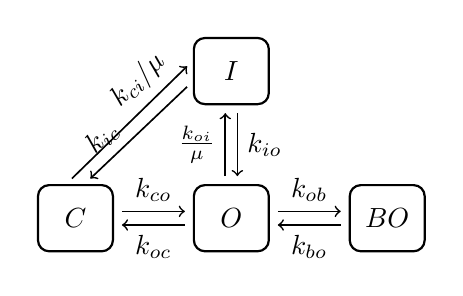
\begin{tikzpicture}[
   font=\sffamily,
   every matrix/.style={ampersand replacement=\&,column sep=1cm,row sep=1cm},
   state/.style={draw,thick,rounded corners,inner sep=.3cm},
   to/.style={->,semithick,shorten >=0.1cm,shorten <=0.1cm},
   Q/.style={->,semithick,sloped,pos=0.700000,shorten >=0.1cm,shorten <=0.1cm},  
   every node/.style={auto}]
\matrix{
\&\node[state] (I) {\parbox{10pt}{\centerline{$I$}}};\&\\
\node[state] (C) {\parbox{10pt}{\centerline{$C$}}};\&\node[state] (O) {\parbox{10pt}{\centerline{$O$}}};\&\node[state] (BO) {\parbox{10pt}{\centerline{$BO$}}};\\
};
\draw[to]  (O.100) to node {$\frac{k_{oi}}{\mu}$} (I.260);
\draw[to]  (O.190) to node {$k_{oc}$} (C.350);
\draw[to]  (O.10) to node {$k_{ob}$} (BO.170);
\draw[to]  (I.280) to node {$k_{io}$} (O.80);
\draw[Q]  (I.195) to node {$k_{ic}$} (C.75);
\draw[to]  (C.10) to node {$k_{co}$} (O.170);
\draw[Q]  (C.105) to node {$k_{ci}/\mu$} (I.165);
\draw[to]  (BO.190) to node {$k_{bo}$} (O.350);
\end{tikzpicture}
\end{center}
\caption{The model represented in Figure  \ref{MOT_mut_L/ICO.pdf} is extended 
to account for the blocker (BO) associated with the open state.}
\label{MOT_mut_L/BICO_O.pdf}
\end{figure}

%\fig[0.7]{MOT_mut_L/BICO_O.pdf}{The model represented in Figure  \ref{MOT_mut_L/ICO.pdf} extended to account for
%the blocker (BO) associated the open state.}


\subsection{Probability density functions using the open state blocker}

We have found a theoretical drug (see $\left(  \ref{mot_in_dr}\right)$) for
the mutation affecting the rates from O to I and from C to I and we want to
assess the drug's usefulness by considering the open probability density
functions. For the wild type case, the probability density functions of the
states present in the Markov model of Figure \ref{MOT_mut_L/ICO.pdf} are
governed by the system%


\begin{align}
\frac{\partial}{\partial v}\left(  a_{o}\rho_{o}\right)   &  =k_{co}\rho
_{c}-\left(  k_{oc}+k_{oi}\right)  \rho_{o}+k_{io}\rho_{i},\nonumber\\
\frac{\partial}{\partial v}\left(  a_{c}\rho_{c}\right)   &  =k_{oc}\rho
_{o}-\left(  k_{co}+k_{ci}\right)  \rho_{c}+k_{ic}\rho_{i},\label{wt_mt_in}\\
\frac{\partial}{\partial v}\left(  a_{c}\rho_{i}\right)   &  =k_{oi}\rho
_{o}-(k_{io}+k_{ic})\rho_{i}+k_{ci}\rho_{c}.\nonumber
\end{align}
In the mutant case, when the open state blocker is added as indicated in Figure
\ref{MOT_mut_L/BICO_O.pdf}, the probability density system is%
\begin{align}
\frac{\partial}{\partial v}\left(  a_{o}\rho_{o}\right)   &  =k_{co}\rho
_{c}-\left(  k_{oc}+\frac{1}{\mu}k_{oi}+k_{ob}\right)  \rho_{o}+k_{io}\rho_{i}%
+k_{bo}\rho_{b},\nonumber\\
\frac{\partial}{\partial v}\left(  a_{c}\rho_{c}\right)   &  =k_{oc}\rho
_{o}-\left(  k_{co}+\frac{1}{\mu}k_{ci}\right)  \rho_{c}+k_{ic}\rho
_{i},\label{mot_dr_123}\\
\frac{\partial}{\partial v}\left(  a_{c}\rho_{i}\right)   &  =\frac{1}{\mu
}k_{oi}\rho_{o}-(k_{io}+k_{ic})\rho_{i}+\frac{1}{\mu}k_{ci}\rho_{c}%
,\nonumber\\
\frac{\partial}{\partial v}\left(  a_{c}\rho_{b}\right)   &  =k_{ob}\rho
_{o}-k_{bo}\rho_{b}.\nonumber
\end{align}
%\K{zzz Skal man ikke i den f\o rste ligningen  i (\ref{mot_dr_123}) ha med leddet $-k_{ob}\rho_{o}$? I s\r{a} fall m\r{a} man vel ogs\r{a} endre fra  $\left(  k_{oc}+\frac{1}{\mu}k_{oi}\right)  \rho_{o}$ til $\left(  k_{oc}+k_{oi}\right)  \rho_{o}$ i den f\o rste ligningen i (\ref{mot_dr_124})?}
%{\bf xxx Glenn: I have corrected the text according to Karoline; can you check the code?}
%\G{This was correct in the code. In general, models are implemented based on the  figure, not the math. (And diagonal entries are computed automatically.)}
As usual, $\rho_{o},\rho_{c},\rho_{i},$ and $\rho_{b}$ denote the probability density
functions of the open, closed, inactivated, and blocked states, respectively,
and the functions of the flux are given by $\left(  \ref{vflux_mot}\right)  .$ By introducing
the drug given by $\left(  \ref{mot_in_dr}\right)  $, we obtain the system
\begin{align}
\frac{\partial}{\partial v}\left(  a_{o}\rho_{o}\right)   &  =k_{co}\rho
_{c}-\left(  k_{oc}+k_{oi}\right)  \rho_{o}+k_{io}\rho_{i}%
+k_{io}\rho_{b},\nonumber\\
\frac{\partial}{\partial v}\left(  a_{c}\rho_{c}\right)   &  =k_{oc}\rho
_{o}-\left(  k_{co}+\frac{1}{\mu}k_{ci}\right)  \rho_{c}+k_{ic}\rho
_{i},\label{mot_dr_124}\\
\frac{\partial}{\partial v}\left(  a_{c}\rho_{i}\right)   &  =\frac{1}{\mu
}k_{oi}\rho_{o}-(k_{io}+k_{ic})\rho_{i}+\frac{1}{\mu}k_{ci}\rho_{c}%
,\nonumber\\
\frac{\partial}{\partial v}\left(  a_{c}\rho_{b}\right)   &  =\left(
1-\mu^{-1}\right)  k_{oi}\rho_{o}-k_{io}\rho_{b}.\nonumber
\end{align}
In Figure \ref{MOT/iocb.pdf}, we show solutions of the wild type system 
$\left(\ref{wt_mt_in}\right)  $, the mutant system, and the mutant system where the
drug is added $\left(  \ref{mot_dr_124}\right)  $. Note that the mutant system
is equal to the wild type system, except for the change of the rates $k_{ci}$
and $k_{oi}$ given by
\begin{align}
\bar{k}_{ci} &  =k_{ci}/\mu,\\
\bar{k}_{oi} &  =k_{oi}/\mu.\nonumber
\end{align}
In Figure \ref{MOT/iocb.pdf},  we compare the open probability density functions of the three models for three
different sets of parameters. In the left panel of Figure \ref{MOT/iocb.pdf},  we show the open probability of the wild type (solid line),
 the mutant ($\mu=10$), and the mutant in the presence of the theoretical open blocker. We see that the effect of the
 mutation is completely repaired by the drug. Other cases are shown in the center and right panels. The effect of the drug is still good but the effect of the mutation is not completely repaired. These observations are confirmed in Table \ref{tab:iocb}.
Furthermore, we have  tested a large variety of parameters and the results 
we show here (center and right panels)  represent the most difficult cases we could find in experiments. 
Therefore, we conclude that the theoretical open state blocker illustrated in Figure  \ref{MOT_mut_L/BICO_O.pdf}
 works very well. 

\fig{MOT/iocb.pdf}{Left panel: All rates equal one. The theoretical drug restores $\rho_o$. Middle panel: As in the left panel, except $k_{co}=10\text{ ms}^{-1}$. 
Right panel:  As in the left panel, except $k_{io}=0.1\text{ ms}^{-1}$. For all three cases, $\mu = 10$.}
%\G{Jeg har testet hver parameter for seg, fra 0.01 til 100. Det er kun disse parameterne som kan gi betydelige avvik, og det blir ikke verre en det vises her, som jo egentlig er ganske bra.}} 

%{\bf xxx Glenn: Can you compute the usual statistical properties of the three cases of 
%Figure \ref{MOT_mut_L/BICO_O.pdf} and put it in a table?}
%\G{This is now Table \ref{tab:iocb}}

\begin{table}  \begin{center}
\begin{tabular}{|c|r|r|r|r|r|r|} \hline
& \multicolumn{2}{c|}{$k=1$} &
\multicolumn{2}{c|}{$k_{co}=10$} &
\multicolumn{2}{c|}{$k_{io}=0.1$}  \\ \cline{2-7}
 & $\pi_o$ & $E_o$ & $\pi_o$ & $E_o$ & $\pi_o$ & $E_o$ \\ \hline
WT&0.333 & 16.366 & 0.476 & 22.995 & 0.083 & -12.867 \\ \hline
MT&0.476 & 23.272 & 0.833 & 31.074 & 0.333 & 17.702 \\ \hline
MT+OB&0.333 & 16.366 & 0.476 & 23.169 & 0.083 & -9.225 \\ \hline
\end{tabular} \end{center}
\caption{Statistical properties of $\rho_o$ for the cases shown in Figure \ref{MOT/iocb.pdf}.\label{tab:iocb}}
\end{table}


\subsection{Stochastic simulations using the open state blocker}

In Figure \ref{MOT/iocb_mc.pdf}, we show simulations using the numerical scheme%
\begin{equation}
v_{n+1}=v_{n}-\Delta t\left(  g_{K}\left(  v_{n}-V_{K}\right)  +\gamma
_{n}g_{Na}(v_{n}-V_{Na}\right)  ), \label{s1000}%
\end{equation}
where the value of the variable $\gamma_{n}$ 
is determined by the Markov model given in
Figure \ref{MOT_mut_L/ICO.pdf}. For the wild type case, the rates $k_{ci}$ and $k_{oi}$
are used and, in the mutant case, the rates $k_{ci}/\mu$ and $k_{oi}%
/\mu$ are used. Furthermore, when the drug is applied in the mutant case, the Markov
model is as illustrated in Figure \ref{MOT_mut_L/BICO_O.pdf}, where the rates of
the drug are given by $\left(\ref{mot_in_dr}\right).$ We observe that, in the
mutant case, the channel does not inactivate and therefore more action
potentials are generated. When the drug is applied, this effect seems to be removed and
the channel again acts more or less as in the wild type case. However, as mentioned above
it is not straightforward to compare solutions based on the stochastic model and therefore we emphasis
the use of probability density functions. 

\fig[0.6]{MOT/iocb_mc.pdf}{Monte Carlo runs of the case shown in the right panel of Figure \ref{MOT/iocb.pdf}.}

\section{Notes}

\begin{enumerate}
\item The derivation of the formula for the mean open time given by (\ref{tau_o}) can be found in many
places (e.g., Keener and Sneyd \cite{KeenerSneyd} or Smith \cite{Smith2002}). 
\end{enumerate}




\chapter[The burst mode]{The burst mode of the mutant sodium channel \label{burst_chap}}

We observed above that the effect of the $\Delta$KPQ mutation of the SCN5A
gene leading to a delayed sodium current can be modeled by increasing the
reaction rates from the inactivated state to the open state and to the
permissible state $C_{0}$. The model gave results at least qualitatively 
similar to the experimental data (see Figure \ref{NaM/mc.pdf}). 

A better-established way of
modeling the effect of the mutation is to introduce a so-called burst mode.
A simple Markov model including a burst mode is illustrated in Figure \ref{burst_prototype}, where the states of the burst mode
are indicated by $\ast$. Note that when the channel is in the burst mode,
there is no inactivated state and therefore the burst mode can be used to model the effect of impaired inactivation.
The reaction rates going from the burst mode to
the normal mode are given by $k^{u}$ (where $u$ stands for up) and the reaction rates from the normal mode
to the burst mode are given by $k^{d}$
(where $d$ stands for down). We assume $k^{d}<<k^{u}$, which means that, for the wild type, 
the probability of being in the burst mode is very small. The probability
of being in the burst mode increases with the mutation severity index $\mu$.
As usual, $\mu=1$ represents the wild type. In the wild type, a channel is basically never in the burst mode and therefore the channel inactivates as it should and no late sodium current is observed. In the mutant case, however, the probability of being in the burst mode is increased. Since there is no inactivated state in the burst mode, the channel fails to inactivate and therefore the probability of being in the open state is increased and therefore we observe a non-negligible late current. This will be illustrated in the numerical computations below.

\begin{figure}[ptb]
\begin{center}
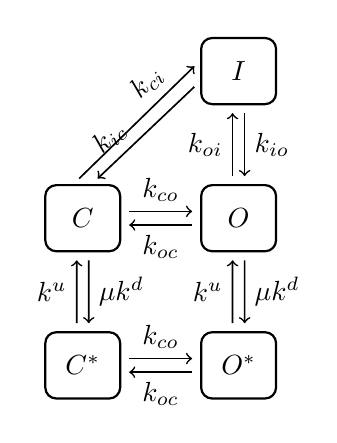
\begin{tikzpicture}[
   font=\sffamily,
   every matrix/.style={ampersand replacement=\&,column sep=1cm,row sep=1cm},
   state/.style={draw,thick,rounded corners,inner sep=.3cm},
   to/.style={->,semithick,shorten >=0.1cm,shorten <=0.1cm},
   Q/.style={->,semithick,sloped,pos=0.700000,shorten >=0.1cm,shorten <=0.1cm},  
   every node/.style={auto}]
\matrix{
\&\node[state] (I) {\parbox{10pt}{\centerline{$I$}}};\\
\node[state] (C) {\parbox{10pt}{\centerline{$C$}}};\&\node[state] (O) {\parbox{10pt}{\centerline{$O$}}};\\
\node[state] (C^{*}) {\parbox{10pt}{\centerline{$C^{*}$}}};\&\node[state] (O^{*}) {\parbox{10pt}{\centerline{$O^{*}$}}};\\
};
\draw[to]  (O^{*}.100) to node {$k^{u}$} (O.260);
\draw[to]  (O^{*}.190) to node {$k_{oc}$} (C^{*}.350);
\draw[to]  (O.280) to node {$\mu k^{d}$} (O^{*}.80);
\draw[to]  (O.100) to node {$k_{oi}$} (I.260);
\draw[to]  (O.190) to node {$k_{oc}$} (C.350);
\draw[to]  (I.280) to node {$k_{io}$} (O.80);
\draw[Q]  (I.195) to node {$k_{ic}$} (C.75);
\draw[to]  (C.10) to node {$k_{co}$} (O.170);
\draw[Q]  (C.105) to node {$k_{ci}$} (I.165);
\draw[to]  (C.280) to node {$\mu k^{d}$} (C^{*}.80);
\draw[to]  (C^{*}.10) to node {$k_{co}$} (O^{*}.170);
\draw[to]  (C^{*}.100) to node {$k^{u}$} (C.260);
\end{tikzpicture}
\end{center}
\caption{Prototypical model of a sodium channel including a burst mode. 
 The model consists of the states $O,I,$ and $C$ of the normal mode and $O^{*}$ and
$C^{*}$ of the burst mode (lower part). }%
\label{burst_prototype}%
\end{figure}



\section{Equilibrium probabilities}

We will start by considering the equilibrium states of the prototypical
model illustrated in Figure \ref{burst_prototype}. By following the usual steps
(see, e.g., page \pageref{9001}) we find
\begin{comment}
The equilibrium solutions are characterized by
the system of equations%
\begin{align}
k_{io}i  &  =k_{oi}o,\text{ }k_{ci}c=k_{ic}i,\text{ }k_{co}c=k_{oc}o,\\
\mu k^{d}c  &  =k^{u}c^{\ast},\text{ }\mu k^{d}o=k^{u}o^{\ast}.
\end{align}
As usual, all variables can be expressed in terms of the open probability,%
\begin{equation}
i=\frac{k_{oi}}{k_{io}}o,\text{ }c=\frac{k_{oc}}{k_{co}}o,\text{ }c^{\ast
}=\frac{\mu k^{d}}{k^{u}}\frac{k_{oc}}{k_{co}}o,\text{ }o^{\ast}=\frac{\mu
k^{d}}{k^{u}}o,
\end{equation}
and, since $o+i+c+c^{\ast}+o^{\ast}=1,$ we have%
\begin{equation}
\left(  1+\frac{k_{oi}}{k_{io}}+\frac{k_{oc}}{k_{co}}+\frac{\mu k^{d}}{k^{u}%
}\frac{k_{oc}}{k_{co}}+\frac{\mu k^{d}}{k^{u}}\right)  o=1
\end{equation}
and therefore
\end{comment}
 the equilibrium probabilities given by%
\begin{align}
o  &  =\frac{1}{1+\frac{k_{oi}}{k_{io}}+\frac{k_{oc}}{k_{co}}+\frac{\mu k^{d}%
}{k^{u}}\frac{k_{oc}}{k_{co}}+\frac{\mu k^{d}}{k^{u}}},\\
i  &  =\frac{\frac{k_{oi}}{k_{io}}}{1+\frac{k_{oi}}{k_{io}}+\frac{k_{oc}%
}{k_{co}}+\frac{\mu k^{d}}{k^{u}}\frac{k_{oc}}{k_{co}}+\frac{\mu k^{d}}{k^{u}%
}},\\
c  &  =\frac{\frac{k_{oc}}{k_{co}}}{1+\frac{k_{oi}}{k_{io}}+\frac{k_{oc}%
}{k_{co}}+\frac{\mu k^{d}}{k^{u}}\frac{k_{oc}}{k_{co}}+\frac{\mu k^{d}}{k^{u}%
}},\\
c^{\ast}  &  =\frac{\frac{k_{oc}}{k_{co}}\frac{\mu k^{d}}{k^{u}}}%
{1+\frac{k_{oi}}{k_{io}}+\frac{k_{oc}}{k_{co}}+\frac{\mu k^{d}}{k^{u}}%
\frac{k_{oc}}{k_{co}}+\frac{\mu k^{d}}{k^{u}}},\\
o^{\ast}  &  =\frac{\frac{\mu k^{d}}{k^{u}}}{1+\frac{k_{oi}}{k_{io}}%
+\frac{k_{oc}}{k_{co}}+\frac{\mu k^{d}}{k^{u}}\frac{k_{oc}}{k_{co}}+\frac{\mu
k^{d}}{k^{u}}}.
\end{align}
Here, we observe that the equilibrium probability of being in the inactivated
state is clearly reduced as the mutation severity index is increased. This is
the effect we wanted, since inactivation is impaired in the
mutation and the effect is modeled by introducing a burst mode that lacks the
inactivated state. Second, we observe that the sum of the open probabilities
given by%
\begin{equation}
o+o^{\ast}=\frac{1+\mu\frac{k^{d}}{k^{u}}}{1+\frac{k_{oi}}{k_{io}}%
+\frac{k_{oc}}{k_{co}}+\mu\frac{k^{d}}{k^{u}}\frac{k_{oc}}{k_{co}}+\mu
\frac{k^{d}}{k^{u}}}%
\end{equation}
is an increasing function of $\mu;$ in fact,%
\begin{equation}
\frac{d}{d\mu}\left(  o+o^{\ast}\right)  =\frac{\frac{k^{d}}{k^{u}}%
\frac{k_{oi}}{k_{io}}}{\left(  1+\frac{k_{oc}}{k_{co}}+\frac{k_{oi}}{k_{io}%
}+\mu\frac{k^{d}}{k^{u}}\frac{k_{oc}}{k_{co}}+\mu\frac{k^{d}}{k^{u}}\right)
^{2}}>0.
\end{equation}
So the model has the two main properties we seek: The equilibrium
probability of being in the inactivated state is reduced and the open probability
is increased.

\bigskip

\section{The mean open time}

We observed above (see page \pageref{mot_many}) that the formula for the mean open time can also
be derived in the presence of several open states. If we generalize the
argument to also take into account the inactivated state, we find that the
mean open time of the Markov model illustrated in Figure \ref{burst_prototype} is given by%
\begin{equation}
\tau_{o,\mu}=\frac{\mu k^{d}+k^{u}}{\mu k^{d}k_{oc}+k^{u}\left(  k_{oc}%
+k_{oi}\right)  }%
\end{equation}
and, since%
\begin{equation}
\frac{d\tau_{o,\mu}}{d\mu}=\frac{k_{oi}k^{d}k^{u}}{\left(  k^{u}k_{oc}+k^{u}k_{oi}+\mu k_{oc}k^{d}\right)  ^{2}},
\end{equation}
the mean open time increases as a function of the mutation severity index.

%\K{zzz Skal man skifte slik fra $k_{oc}$ og $k_{oi}$ til $k_{co}$ og $k_{io}$
%n\r{a}r man deriverer?}

\bigskip

\section{An optimal theoretical open state blocker}

\begin{figure}[ptb]
\begin{center}
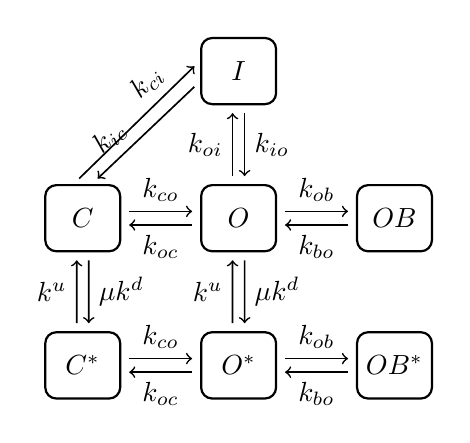
\begin{tikzpicture}[
   font=\sffamily,
   every matrix/.style={ampersand replacement=\&,column sep=1cm,row sep=1cm},
   state/.style={draw,thick,rounded corners,inner sep=.3cm},
   to/.style={->,semithick,shorten >=0.1cm,shorten <=0.1cm},
   Q/.style={->,semithick,sloped,pos=0.700000,shorten >=0.1cm,shorten <=0.1cm},  
   every node/.style={auto}]
\matrix{
\&\node[state] (I) {\parbox{10pt}{\centerline{$I$}}};\&\\
\node[state] (C) {\parbox{10pt}{\centerline{$C$}}};\&\node[state] (O) {\parbox{10pt}{\centerline{$O$}}};\&\node[state] (OB) {\parbox{10pt}{\centerline{$OB$}}};\\
\node[state] (C^{*}) {\parbox{10pt}{\centerline{$C^{*}$}}};\&\node[state] (O^{*}) {\parbox{10pt}{\centerline{$O^{*}$}}};\&\node[state] (OB^{*}) {\parbox{10pt}{\centerline{$OB^{*}$}}};\\
};
\draw[to]  (O^{*}.100) to node {$k^{u}$} (O.260);
\draw[to]  (O^{*}.10) to node {$k_{ob}$} (OB^{*}.170);
\draw[to]  (O^{*}.190) to node {$k_{oc}$} (C^{*}.350);
\draw[to]  (O.280) to node {$\mu k^{d}$} (O^{*}.80);
\draw[to]  (O.100) to node {$k_{oi}$} (I.260);
\draw[to]  (O.190) to node {$k_{oc}$} (C.350);
\draw[to]  (O.10) to node {$k_{ob}$} (OB.170);
\draw[to]  (I.280) to node {$k_{io}$} (O.80);
\draw[Q]  (I.195) to node {$k_{ic}$} (C.75);
\draw[to]  (C.10) to node {$k_{co}$} (O.170);
\draw[Q]  (C.105) to node {$k_{ci}$} (I.165);
\draw[to]  (C.280) to node {$\mu k^{d}$} (C^{*}.80);
\draw[to]  (OB.190) to node {$k_{bo}$} (O.350);
\draw[to]  (OB^{*}.190) to node {$k_{bo}$} (O^{*}.350);
\draw[to]  (C^{*}.10) to node {$k_{co}$} (O^{*}.170);
\draw[to]  (C^{*}.100) to node {$k^{u}$} (C.260);
\end{tikzpicture}
\end{center}
\caption{Prototypical model of a sodium channel including a burst mode and an open state blocker. 
 The model consists of the states $O,I,C,$ and $OB$ of the normal mode and $O^{*},C^{*},$ and $OB^*$ of the burst mode (lower part). 
 The states $OB$ and $OB^*$ represent the open blocker and we assume that the rates characterizing the blocker are the same in the normal and burst modes.}%
\label{burst_prototype_drg}%
\end{figure}


Our aim is now to define an open state drug that can repair both the
equilibrium open probability and the mean open time. The structure of the open
state blocker is given in Figure \ref{burst_prototype_drg} and the equilibrium total open probability is now
given by 
\begin{comment}
the following system of equations:%
\begin{align*}
k_{io}i  &  =k_{oi}o,\text{ }k_{ci}c=k_{ic}i,\text{ }k_{co}c=k_{oc}o,\text{
}k_{bo}b=k_{ob}o,\\
\mu k^{d}c  &  =k^{u}c^{\ast},\text{ }\mu k^{d}o=k^{u}o^{\ast},\text{ }%
k_{bo}b^{\ast}=k_{ob}o^{\ast}.
\end{align*}
Since%
\begin{equation*}
i=\frac{k_{oi}}{k_{io}}o,\text{ }c=\frac{k_{oc}}{k_{co}}o,\text{ }c^{\ast
}=\frac{\mu k^{d}}{k^{u}}\frac{k_{oc}}{k_{co}}o,\text{ }o^{\ast}=\frac{\mu
k^{d}}{k^{u}}o,\text{ }b=\frac{k_{ob}}{k_{bo}}o,\text{ }b^{\ast}=\frac{k_{ob}%
}{k_{bo}}\frac{\mu k^{d}}{k^{u}}o
\end{equation*}
and $o+i+c+c^{\ast}+o^{\ast}+b+b^{\ast}=1,$ 
we obtain the total open probability%
\end{comment}
\begin{equation}
\left(  o+o^{\ast}\right)  _{\mu,d}=\frac{1+\mu\frac{k^{d}}{k^{u}}}{1+\frac
{k_{oi}}{k_{io}}+\frac{k_{oc}}{k_{co}}+\mu\frac{k^{d}}{k^{u}}\frac{k_{oc}%
}{k_{co}}+\mu\frac{k^{d}}{k^{u}}+\frac{k_{ob}}{k_{bo}}\left(  1+\frac{\mu
k^{d}}{k^{u}}\right)  }. \label{o300}%
\end{equation}
Furthermore, the mean open time is now given by%
\begin{equation}
\tau_{o,\mu,d}=\frac{\mu k^{d}+k^{u}}{\mu k^{d}\left(  k_{oc}+k_{ob}\right)
+k^{u}\left(  k_{oc}+k_{oi}+k_{ob}\right)  }, \label{mot300}%
\end{equation}
where the subscript $d$ is used to remind us that this concerns the case where
the theoretical drug has been applied.

\bigskip

The task at hand is now to tune the drug such that the equilibrium open
probability and the mean open time given by $\left(  \ref{o300}\right)  $ and
$\left(  \ref{mot300}\right)  $, respectively, are as close as possible to the equilibrium open
probability and the mean open time of the wild type. We regard the parameters
$k_{ob}$ and $k_{bo}$ as the unknowns and we want to solve the following
$2\times2$ system of equations:%
\begin{align}
\frac{1+\mu\frac{k^{d}}{k^{u}}}{1+\frac{k_{oi}}{k_{io}}+\frac{k_{oc}}{k_{co}%
}+\mu\frac{k^{d}}{k^{u}}\frac{k_{oc}}{k_{co}}+\mu\frac{k^{d}}{k^{u}}%
+\frac{k_{ob}}{k_{bo}}\left(  1+\mu\frac{k^{d}}{k^{u}}\right)  }  &  =\frac
{1+\frac{k^{d}}{k^{u}}}{1+\frac{k_{oi}}{k_{io}}+\frac{k_{oc}}{k_{co}}+\frac{k^{d}}{k^{u}}%
\frac{k_{oc}}{k_{co}}+\frac{k^{d}}{k^{u}}},\label{dr300}\\
\frac{\mu k^{d}+k^{u}}{\mu k^{d}\left(  k_{oc}+k_{ob}\right)  +k^{u}\left(
k_{oc}+k_{oi}+k_{ob}\right)  }  &  =\frac{k^{d}+k^{u}}{k^{d}k_{oc}%
+k^{u}\left(  k_{oc}+k_{oi}\right)  }, \label{dr301}%
\end{align}
where the latter equation determines the on rate, $k_{ob},$ of the drug,%
\begin{equation}
k_{ob}=\left(  \mu-1\right)  \frac{k^{d}k^{u}k_{oi}}{\left(  k^{u}+\mu
k^{d}\right)  \left(  k^{u}+k^{d}\right)  }, \label{kob300}%
\end{equation}
and we note that, in the case of $\mu=1,$ the  drug is completely turned off,
which is reasonable. Since $k_{ob}$ is known, the off rate of the drug can be
computed by solving $\left(  \ref{dr300}\right).$ If we define%
\begin{equation}
A=\frac{k_{ob}}{k_{bo}},
\end{equation}
we find from $\left(  \ref{dr300}\right)$  
\begin{equation}
A=(\mu-1)\frac{k_{oi}}{k_{io}}  \frac{k^{u}k^{d}}{\left(  \mu k^{d}+k^{u}\right)  \left(  k^{d}%
+k^{u}\right)  \label{Akbo}}
\end{equation}
and then the off rate of the drug is given by%
\begin{equation}
k_{bo}=A^{-1}k_{ob}=k_{io} \label{kbo300}
\end{equation}
which is the same as we have in the prototypical model given in 
Figure \ref{MOT_mut_L/BICO_O.pdf}; see (\ref{mot_in_dr}) on page \pageref{mot_in_dr}.


\bigskip

\section{Numerical experiments}

\graytable{l}{
{|c|c|} \hline
$\mu$ & 20 \\ \hline
$k_u$ & 0.0001 $\rm{ms^{-1}}$\\ \hline
$k_d$ & 0.001 $\rm{ms^{-1}}$\\ \hline
$k_{ob}$ & 0.0286 $\rm{ms^{-1}}$\\ \hline
$k_{bo}$ &0.000824 $\rm{ms^{-1}}$\\ \hline
}{Values of the parameters used in the model in Figure \ref{burst_prototype_drg}.
The remaining rates  are as in Table \ref{markov_rates}.
\label{tab:burst_ob}}

The purpose of this section is to show how the burst mode can be used to represent impaired inactivation and how the theoretical drug derived above works. 

\subsection{Representation of the late sodium current using the burst mode model}

As discussed in Chapter \ref{simple_Na}, impaired inactivation leads to a late sodium current (see Figure \ref{NaM/mc.pdf}). Here, we will see that this effect can also be obtained using a Markov model of the form indicated in Figure \ref{burst_prototype}. In Figure \ref{NaB/current.pdf}, we repeat the computations reported in Figure \ref{NaM/mc.pdf}, using the Markov model of Figure \ref{burst_prototype}. The parameters used in this computation are given in Table \ref{tab:burst_ob}. We observe from Figure \ref{NaB/current.pdf} that $\mu=20$ seems to represent the late current of Figure \ref{NaM/mc.pdf} fairly well. 
 
 \subsection{The open state blocker repairs the effect of the mutation}

In Figure \ref{NaB/current.pdf}, we show the late current for the wild type, the mutant $\mu=20$, and the drug using the optimal open state blocker defined by (\ref{kob300}) and (\ref{kbo300}). We observe that the late current induced by the mutation is  repaired by the open state blocker. The statistics of the open probability density function (for the wild type, the mutant ($\mu=20$), and the mutant where the drug has been applied) are given in Table \ref{tab:burst_stat} and  
the corresponding probability density functions are shown in Figure \ref{NaB/ob.pdf}. Again we note that the open blocker repairs the main features of the solution.



\fig{NaB/current.pdf}{Currents computed using the Markov model illustrated in Figure \ref{burst_prototype_drg}. 
The simulations are based on averages of 10,000 runs. As expected, the open blocker asymptotically repairs the late current. }

%\fig{NaB/current_zoom.pdf}{Just to illustrate that things work as expected, we might not want to use this one.}

\fig{NaB/ob.pdf}{Stationary probability density functions computed using the Markov model illustrated in Figure
\ref{burst_prototype_drg}. The open probability density function is given in the left panel and the probability density function of the sum of non-conducting states is given in the right panel. We observe that the open blocker repairs most parts of the probability density functions.}

\begin{table}  \begin{center}
\begin{tabular}{|r|r|r|r|r|} \hline
$\mu$ & $\pi_o$ & $\pi_n$ & $E_o$ & $E_n$ \\ \hline
1 & 0.59 & 0.41 & 31.2 & -54.2 \\ \hline
20 & 0.96 & 0.04 & 33.1 & -52.8 \\ \hline
50 & 0.98 & 0.02 & 33.1 & -51.3 \\ \hline
100 & 0.99 & 0.01 & 33.2 & -49.8 \\ \hline
20+OB & 0.46 & 0.54 & 30.2 & -57.9 \\ \hline
\end{tabular} \end{center}
\caption{Statistics of the stationary probability density functions computed using the Markov model illustrated in Figure
\ref{burst_prototype_drg}. The subscript $o$ refers to open states and the subscript $n$ refers to non-conducting states.
 \label{tab:burst_stat}}
\end{table}



\section{A more sophisticated Markov model \label{sophisticated}}

The Markov model presented in Figure \ref{burst_prototype} above has a structure that is a bit simpler than
the Markov model commonly used to model the sodium channel. A more common structure is given in 
Figure \ref{wtreac330}. This is the model we studied in Chapter \ref{simple_Na}. When a burst mode is added to it, the Markov model obtains the form illustrated in Figure \ref{burst}.


\begin{figure}[ptb]
\begin{center}
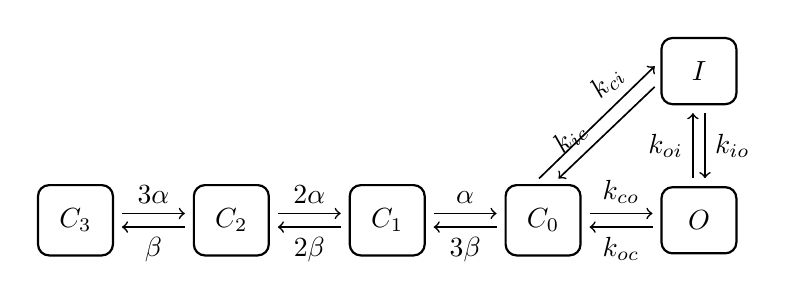
\begin{tikzpicture}[
   font=\sffamily,
   every matrix/.style={ampersand replacement=\&,column sep=1cm,row sep=1cm},
   state/.style={draw,thick,rounded corners,inner sep=.3cm},
   to/.style={->,semithick,shorten >=0.1cm,shorten <=0.1cm},
   Q/.style={->,semithick,sloped,pos=0.700000,shorten >=0.1cm,shorten <=0.1cm},  
   every node/.style={auto}]
\matrix{
\&\&\&\&\node[state] (I) {\parbox{10pt}{\centerline{$I$}}};\\
\node[state] (C_{3}) {\parbox{10pt}{\centerline{$C_{3}$}}};\&\node[state] (C_{2}) {\parbox{10pt}{\centerline{$C_{2}$}}};\&\node[state] (C_{1}) {\parbox{10pt}{\centerline{$C_{1}$}}};\&\node[state] (C_{0}) {\parbox{10pt}{\centerline{$C_{0}$}}};\&\node[state] (O) {\parbox{10pt}{\centerline{$O$}}};\\
};
\draw[to]  (O.100) to node {$k_{oi}$} (I.260);
\draw[to]  (O.190) to node {$k_{oc}$} (C_{0}.350);
\draw[to]  (I.280) to node {$k_{io}$} (O.80);
\draw[Q]  (I.195) to node {$k_{ic}$} (C_{0}.75);
\draw[to]  (C_{0}.10) to node {$k_{co}$} (O.170);
\draw[Q]  (C_{0}.105) to node {$k_{ci}$} (I.165);
\draw[to]  (C_{0}.190) to node {$3\beta$} (C_{1}.350);
\draw[to]  (C_{1}.10) to node {$\alpha$} (C_{0}.170);
\draw[to]  (C_{1}.190) to node {$2\beta$} (C_{2}.350);
\draw[to]  (C_{2}.10) to node {$2\alpha$} (C_{1}.170);
\draw[to]  (C_{2}.190) to node {$\beta$} (C_{3}.350);
\draw[to]  (C_{3}.10) to node {$3\alpha$} (C_{2}.170);
\end{tikzpicture}
\end{center}
\caption{Typical Markov model of a wild type sodium channel consisting of an open
state $(O)$, an inactivated state $(I)$, and four closed states $(C_{0}%
,C_{1},C_{2}, \text{ and }C_{3})$. This model was analyzed in Chapter \ref{simple_Na}.}%
\label{wtreac330}%
\end{figure}



\begin{figure}[ptb]
\begin{center}
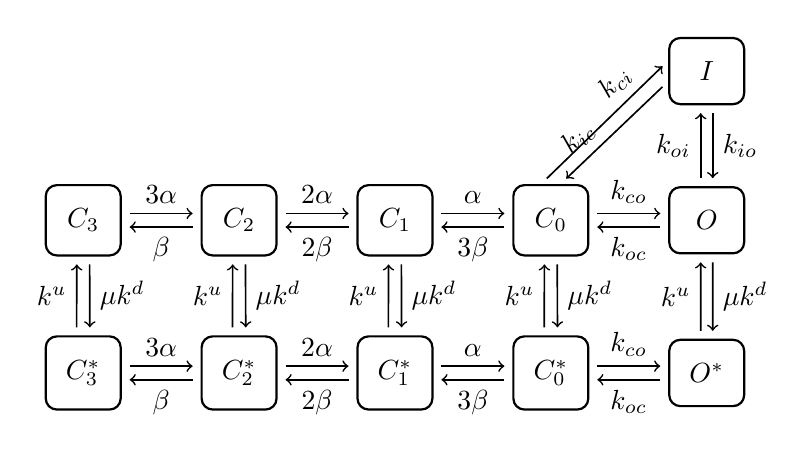
\begin{tikzpicture}[
   font=\sffamily,
   every matrix/.style={ampersand replacement=\&,column sep=1cm,row sep=1cm},
   state/.style={draw,thick,rounded corners,inner sep=.3cm},
   to/.style={->,semithick,shorten >=0.1cm,shorten <=0.1cm},
   Q/.style={->,semithick,sloped,pos=0.700000,shorten >=0.1cm,shorten <=0.1cm},  
   every node/.style={auto}]
\matrix{
\&\&\&\&\node[state] (I) {\parbox{10pt}{\centerline{$I$}}};\\
\node[state] (C_{3}) {\parbox{10pt}{\centerline{$C_{3}$}}};\&\node[state] (C_{2}) {\parbox{10pt}{\centerline{$C_{2}$}}};\&\node[state] (C_{1}) {\parbox{10pt}{\centerline{$C_{1}$}}};\&\node[state] (C_{0}) {\parbox{10pt}{\centerline{$C_{0}$}}};\&\node[state] (O) {\parbox{10pt}{\centerline{$O$}}};\\
\node[state] (C_{3}^{*}) {\parbox{10pt}{\centerline{$C_{3}^{*}$}}};\&\node[state] (C_{2}^{*}) {\parbox{10pt}{\centerline{$C_{2}^{*}$}}};\&\node[state] (C_{1}^{*}) {\parbox{10pt}{\centerline{$C_{1}^{*}$}}};\&\node[state] (C_{0}^{*}) {\parbox{10pt}{\centerline{$C_{0}^{*}$}}};\&\node[state] (O^{*}) {\parbox{10pt}{\centerline{$O^{*}$}}};\\
};
\draw[to]  (O^{*}.100) to node {$k^{u}$} (O.260);
\draw[to]  (O^{*}.190) to node {$k_{oc}$} (C_{0}^{*}.350);
\draw[to]  (O.280) to node {$\mu k^{d}$} (O^{*}.80);
\draw[to]  (O.100) to node {$k_{oi}$} (I.260);
\draw[to]  (O.190) to node {$k_{oc}$} (C_{0}.350);
\draw[to]  (I.280) to node {$k_{io}$} (O.80);
\draw[Q]  (I.195) to node {$k_{ic}$} (C_{0}.75);
\draw[to]  (C_{0}.10) to node {$k_{co}$} (O.170);
\draw[Q]  (C_{0}.105) to node {$k_{ci}$} (I.165);
\draw[to]  (C_{0}.190) to node {$3\beta$} (C_{1}.350);
\draw[to]  (C_{0}.280) to node {$\mu k^{d}$} (C_{0}^{*}.80);
\draw[to]  (C_{1}.10) to node {$\alpha$} (C_{0}.170);
\draw[to]  (C_{1}.190) to node {$2\beta$} (C_{2}.350);
\draw[to]  (C_{1}.280) to node {$\mu k^{d}$} (C_{1}^{*}.80);
\draw[to]  (C_{2}.10) to node {$2\alpha$} (C_{1}.170);
\draw[to]  (C_{2}.190) to node {$\beta$} (C_{3}.350);
\draw[to]  (C_{2}.280) to node {$\mu k^{d}$} (C_{2}^{*}.80);
\draw[to]  (C_{3}.10) to node {$3\alpha$} (C_{2}.170);
\draw[to]  (C_{3}.280) to node {$\mu k^{d}$} (C_{3}^{*}.80);
\draw[to]  (C_{0}^{*}.10) to node {$k_{co}$} (O^{*}.170);
\draw[to]  (C_{0}^{*}.100) to node {$k^{u}$} (C_{0}.260);
\draw[to]  (C_{0}^{*}.190) to node {$3\beta$} (C_{1}^{*}.350);
\draw[to]  (C_{1}^{*}.100) to node {$k^{u}$} (C_{1}.260);
\draw[to]  (C_{1}^{*}.10) to node {$\alpha$} (C_{0}^{*}.170);
\draw[to]  (C_{1}^{*}.190) to node {$2\beta$} (C_{2}^{*}.350);
\draw[to]  (C_{2}^{*}.100) to node {$k^{u}$} (C_{2}.260);
\draw[to]  (C_{2}^{*}.10) to node {$2\alpha$} (C_{1}^{*}.170);
\draw[to]  (C_{2}^{*}.190) to node {$\beta$} (C_{3}^{*}.350);
\draw[to]  (C_{3}^{*}.100) to node {$k^{u}$} (C_{3}.260);
\draw[to]  (C_{3}^{*}.10) to node {$3\alpha$} (C_{2}^{*}.170);
\end{tikzpicture}
\end{center}\caption{Markov model of the sodium channel. The model consists of the states
$O,I,C_{0},C_{1},C_{2},$ and $C_{3}$ of the normal mode and $O^{*},C^{*}%
_{0},C^{*}_{1},C^{*}_{2},$ and $C^{*}_{3}$ of the burst mode (lower part). Note
that there is no inactivated state in the burst mode and that $\mu$ denotes
the mutation severity index. A larger value of $\mu$ increases the probability
of moving from the normal (upper) mode to the burst (lower) mode.}%
\label{burst}%
\end{figure}

To understand how the burst mode changes the properties of the model,
it is of interest to compute the equilibrium probabilities. 
%\begin{comment}
The equilibrium state of the model presented in Figure \ref{burst} is
characterized by the following system of equations:%
\begin{equation}%
\begin{array}
[c]{ccc}%
k_{ci}c_{0}=k_{ic}i, & k_{oi}o=k_{io}i, & k_{co}c_{0}=k_{oc}o,\\
3\beta c_{0}=\alpha c_{1}, & 2\alpha c_{2}=2\beta c_{1}, & 3\alpha c_{3}=\beta c_{2},\\
k^{u}o^{\ast}=\mu k^{d}o, & k^{u}c_{0}^{\ast}=\mu k^{d}c_{0}, & k^{u}%
c_{1}^{\ast}=\mu k^{d}c_{1},\\
k^{u}c_{2}^{\ast}=\mu k^{d}c_{2}, & k^{u}c_{3}^{\ast}=\mu k^{d}c_{3}. &
\end{array}
\label{ep1}
\end{equation}
It follows that%
\begin{align*}
i &  =\frac{k_{oi}}{k_{io}}o,\text{ }c_{0}=\frac{k_{oc}}{k_{co}}o,\text{ }\\
c_{1} &  =\frac{3\beta}{\alpha}\frac{k_{oc}}{k_{co}}o,\text{ }c_{2}%
=\frac{3\beta^{2}}{\alpha^{2}}\frac{k_{oc}}{k_{co}}o,\text{ }c_{3}=\frac
{\beta^{3}}{\alpha^{3}}\frac{k_{oc}}{k_{co}}o,\\
o^{\ast} &  =\mu\frac{k^{d}}{k^{u}}o,c_{0}^{\ast}=\mu\frac{k^{d}}{k^{u}}%
\frac{k_{oc}}{k_{co}}o,c_{1}^{\ast}=\mu\frac{3\beta}{\alpha}\frac{k^{d}}%
{k^{u}}\frac{k_{oc}}{k_{co}}o,\\
c_{2}^{\ast} &  =\mu\frac{3\beta^{2}}{\alpha^{2}}\frac{k^{d}}{k^{u}}%
\frac{k_{oc}}{k_{co}}o,c_{3}^{\ast}=\mu\frac{\beta^{3}}{\alpha^{3}}\frac
{k^{d}}{k^{u}}\frac{k_{oc}}{k_{co}}o
\end{align*}
and, since the sum of the probabilities equals one, we have%
%\end{comment}
\[
o\left(  \mu\right)  =\frac{1}{\frac{k_{oi}}{k_{io}}+\left(  1+\mu\frac{k^{d}%
}{k^{u}}\right)  \left(  1+\frac{k_{oc}}{k_{co}}\left(  1+\beta/\alpha\right)
^{3}\right)  }
\]
and
\[
o\left(  \mu\right)  +o^{\ast}\left(  \mu\right)  =\frac{1+\mu\frac{k^{d}%
}{k^{u}}}{\frac{k_{oi}}{k_{io}}+\left(  1+\mu\frac{k^{d}}{k^{u}}\right)
\left(  1+\frac{k_{oc}}{k_{co}}\left(  1+\beta/\alpha\right)  ^{3}\right)  }.%
\]
Therefore,
\[
\frac{d}{d\mu}\left(  o\left(  \mu\right)  +o^{\ast}\left(  \mu\right)
\right)  =\frac{\frac{k_{oi}}{k_{io}}\frac{k^{d}}{k^{u}}}{\left(  \frac
{k_{oi}}{k_{io}}+\left(  1+\frac{k_{oc}}{k_{co}}\left(  1+\beta/\alpha\right)
^{3}\right)  \left(  1+\mu\frac{k^{d}}{k^{u}}\right)  \right)  ^{2}}>0,%
\]
so the total open probability increases as the mutation severity index
$\mu$ increases. This will lead to a sustained sodium current characteristic
of the mutation under consideration. 

It is also interesting to see how the mutation severity index changes the
probability of being in the normal or burst mode. To understand
this, we define $b$ and $b^{\ast}$ as the sum of the probabilities in the
normal and burst modes, respectively. By using the equilibrium probabilities
derived above, we obtain
\[
\frac{b^{\ast}}{b}=\frac{o^{\ast}+c_{0}^{\ast}+c_{1}^{\ast}+c_{2}^{\ast}%
+c_{3}^{\ast}}{o+c_{0}+c_{1}+c_{2}+c_{3}+i}=\mu\frac{k^{d}}{k^{u}}%
\frac{1+\frac{k_{oc}}{k_{co}}\left(  1+\beta/\alpha\right)  ^{3}}%
{\frac{k_{oi}}{k_{io}}+1+\frac{k_{oc}}{k_{co}}\left(  1+\beta/\alpha\right)
^{3}}%
\]
and thus the probability of being in the burst mode increases as the mutation
severity index increases.

\bigskip

\section[Numerical experiments; burst mode]{Numerical experiments illustrating the effect of the burst mode}

\graytable{l}{
{|c|c|} \hline
$\mu$ & 1,10,30,100 \\ \hline
$k_u$ & 0.1 $\rm{ms^{-1}}$\\ \hline
$k_d$ & 0.01 $\rm{ms^{-1}}$\\ \hline
%$k_{ob}$ &  0.2196 $\rm{ms^{-1}}$\\ \hline
%$k_{bo}$ &0.0001578 $\rm{ms^{-1}}$\\ \hline
}{Values of the parameters used in the model in Figure \ref{burst}.
%\ref{burstdrg}.
The remaining rates  are as in Table \ref{markov_rates} on page \pageref{markov_rates}. \label{tab:burst_param}
}


The effect of increasing the mutation severity index of the Markov model given in Figure \ref{burst} is shown in
 Figure \ref{NaB/pdf3.pdf} using the parameters given in Table \ref{tab:burst_param}.
  %In the computations we use the parameters $k_u=0.1, k_d = 0.01$ and the mutation severity index is $\mu=1,10,30,100$ where $\mu=1$ (solid line) represents the wild type. 
 The associated currents are shown in Figure
 \ref{NaB/mc.pdf} and we note that when the mutation severity index increases, there is a significant late sodium current.
 
\fig{NaB/pdf3.pdf}{ The probability density functions of the open, closed, and inactivated states for the
burst mode model. The mutation severity index is given by $\mu=10,$ $30,$ and $100$ and the black line represents the wild type.
Note that we only show solutions for the values of the transmembrane potential where the solutions differ as a result of the mutations.}

%\fig{NaB/mc.pdf}{\G{Top trace is WT, the other ones MT, with the lowest corresponding to $\mu=100$.} 
%Current from the burst model. Stronger mutations leads to slower closing of the channel.}


\begin{figure}[p]\centering
\vbox{
\includegraphics[width=0.9\linewidth]{NaB/mc.pdf}
\includegraphics[width=0.7\linewidth]{NaM/Bennet.png}
}
\caption{Currents computed using the Markov model including the burst mode (see Figure \ref{burst}). Top panel: Current for $\mu=1,$ $10,$ $30,$ $100$. Each trace is an average of 10,000 Monte Carlo runs and the current is computed by  $I=g_{Na} P_o (v-V_{Na})$, with the transmembrane potential at $v=0$ mV. The currents are normalized so that the wild type current peaks at -1. Here $V_{Na} = 45$ mV and $g_{Na} = 1$ mS/$\mbox{cm}^2$.  The lower figures are from Bennett et al. \cite{Bennett1995}.\label{NaB/mc.pdf}}
\end{figure}


%\begin{table}  \begin{center}
%\begin{tabular}{|r|r|r|r|r|r|r|} \hline
%$\mu$ & $\pi_o$ & $\pi_c$ & $\pi_i$ & $\rho_o$ & $\rho_c$ & $\rho_i$ \\ \hline
%1 & 0.00006 & 0.99961 & 0.00033 & -53.2 & -84.9 & -73.4 \\ \hline
%10 & 0.00008 & 0.99967 & 0.00024 & -26.1 & -84.9 & -67.5 \\ \hline
%30 & 0.00012 & 0.99969 & 0.00019 & -8.3 & -84.9 & -61.0 \\ \hline
%100 & 0.00022 & 0.99963 & 0.00015 & 10.5 & -84.9 & -54.2 \\ \hline
%\end{tabular} \end{center}
%\caption{ Expected values of the transmembrane potential for open, closed or inactivated
%states for increasing values of the mutation severity index $\mu$.} \label{tab:burst}
%\end{table}
\begin{table}  \begin{center}
\begin{tabular}{|r|r|r|r|r|} \hline
$\mu$ & $1000 \times \pi_o$ & $\pi_n$ & $E_o$ & $E_c$ \\ \hline
1 & 0.05738 &  0.99994 & -53.2 & -84.9 \\ \hline
10 & 0.08435 & 0.99992 & -26.1 & -84.9 \\ \hline
30 & 0.12109 & 0.99983 & -8.3 & -84.9 \\ \hline
100 & 0.22305 & 0.99978 & 10.5 & -84.9 \\ \hline
30+OB & 0.05490&0.99995 & -57.0 & -84.9 \\ \hline
\end{tabular} \end{center}
\caption{Probabilities and expected values of the transmembrane potential for open and non-conducting states for increasing values of the mutation severity index $\mu$.} \label{tab:burst}
\end{table}


%xxx Glenn xxx: repeat experiments of the previous model. That is repeat figure 11.3, table 11.2, figure 11.4.



\section[Theoretical drug for the burst mode model]{A theoretical drug for the
mutation represented by the burst mode}

 In the simplified Markov model presented in Figure \ref{burst_prototype} above, we saw
that an open blocker was able to repair the effect of the mutation.
Now the Markov model is extended (see Figure \ref{burst}), but it is reasonable to
believe that an open blocker is still the best alternative, since both the open
probability and the mean open time are affected by the mutation. We consider
the Markov model given in Figure \ref{burstdrg}, where an open blocker is added to both
the open states of the Markov model given in Figure \ref{burst}. 
\begin{comment}
The equilibrium state
of the Markov model given in Figure \ref{burstdrg} is characterized by%
\begin{equation}%
\begin{array}
[c]{ccc}%
k_{ci}c_{0}=k_{ic}i, & k_{oi}o=k_{io}i, & k_{co}c_{0}=k_{oc}o,\\
3\beta c_{0}=\alpha c_{1}, & 2\alpha c_{2}=2\beta c_{1}, & 3\alpha c_{3}=\beta
c_{2},\\
k^{u}o^{\ast}=\mu k^{d}o, & k^{u}c_{0}^{\ast}=\mu k^{d}c_{0}, & k^{u}%
c_{1}^{\ast}=\mu k^{d}c_{1},\\
k^{u}c_{2}^{\ast}=\mu k^{d}c_{2}, & k^{u}c_{3}^{\ast}=\mu k^{d}c_{3}, & \\
k_{ob}o=k_{bo}b, & k_{ob}o^{\ast}=k_{bo}b^{\ast}. &
\end{array}
\end{equation}
\end{comment}
By following our usual procedure, we find that%
\begin{comment}
\begin{align*}
i &  =\frac{k_{oi}}{k_{io}}o,\text{ }c_{0}=\frac{k_{oc}}{k_{co}}o,\text{ }\\
c_{1} &  =\frac{3\beta}{\alpha}\frac{k_{oc}}{k_{co}}o,\text{ }c_{2}%
=\frac{3\beta^{2}}{\alpha^{2}}\frac{k_{oc}}{k_{co}}o,\text{ }c_{3}=\frac
{\beta^{3}}{\alpha^{3}}\frac{k_{oc}}{k_{co}}o,\\
o^{\ast} &  =\mu\frac{k^{d}}{k^{u}}o,c_{0}^{\ast}=\mu\frac{k^{d}}{k^{u}}%
\frac{k_{oc}}{k_{co}}o,c_{1}^{\ast}=\mu\frac{3\beta}{\alpha}\frac{k^{d}}%
{k^{u}}\frac{k_{oc}}{k_{co}}o,\\
c_{2}^{\ast} &  =\mu\frac{3\beta^{2}}{\alpha^{2}}\frac{k^{d}}{k^{u}}%
\frac{k_{oc}}{k_{co}}o,c_{3}^{\ast}=\mu\frac{\beta^{3}}{\alpha^{3}}\frac
{k^{d}}{k^{u}}\frac{k_{oc}}{k_{co}}o,\\
b &  =\frac{k_{ob}}{k_{bo}}o,b^{\ast}=\mu\frac{k_{ob}}{k_{bo}}\frac{k^{d}%
}{k^{u}}o,
\end{align*}
\newline and, since the sum of the probabilities equals one, we have
\end{comment}
\[
\left(  o+o^{\ast}\right)  _{\mu,d}=\frac{1+\mu\frac{k^{d}}{k^{u}}}%
{\frac{k_{ob}}{k_{bo}}\left(  1+\mu\frac{k^{d}}{k^{u}}\right)  +\frac{k_{oi}%
}{k_{io}}+\left(  1+\mu\frac{k^{d}}{k^{u}}\right)  \left(  1+\frac{k_{oc}%
}{k_{co}}\left(  1+\beta/\alpha\right)  ^{3}\right)  }.
\]
The associated mean open time is given by%
\begin{equation}
\tau_{o,\mu,d}=\frac{\mu k^{d}+k^{u}}{\mu k^{d}\left(  k_{oc}+k_{ob}\right)
+k^{u}\left(  k_{oc}+k_{oi}+k_{ob}\right)  }.
\end{equation}
We now want to tune the drug characterized by the two parameters $k_{ob}$
and $k_{bo}$ such that
\[
\left(  o+o^{\ast}\right)  _{\mu,d}\approx\left(  o+o^{\ast}\right)  _{wt}%
\]
and%
\[
\tau_{o,\mu,d}\approx\tau_{o,wt},%
\]
where the subscript {\it wt} denotes wild type values. As above, we have two equations
for the two unknowns  $k_{ob}$ and $k_{bo}$ and the solution is given by%
\begin{equation}
k_{ob}=\left(  \mu-1\right)  \frac{k^{d}k^{u}k_{oi}}{\left(  k^{u}+\mu
k^{d}\right)  \left(  k^{u}+k^{d}\right)  } \label{na_drug_ob}
\end{equation}
and%
\begin{equation}
k_{bo}=A^{-1}k_{ob},
\end{equation}
where%
\begin{equation}
A=\frac{k_{oi}}{k_{io}}k^{u}k^{d}\frac{\mu-1}{\left(  \mu k^{d}+k^{u}\right)
\left(  k^{d}+k^{u}\right)  }.
\end{equation}
So we obtain
\begin{equation}
k_{bo}=k_{io}. \label{na_drug_bo}
\end{equation}
We note that the formulas for the optimal open blocker for the Markov model
given in Figure \ref{burstdrg} are exactly the same as for the open blocker of the prototype Markov
model given in Figure \ref{burst_prototype_drg}.


\begin{figure}[ptb]
\begin{center}
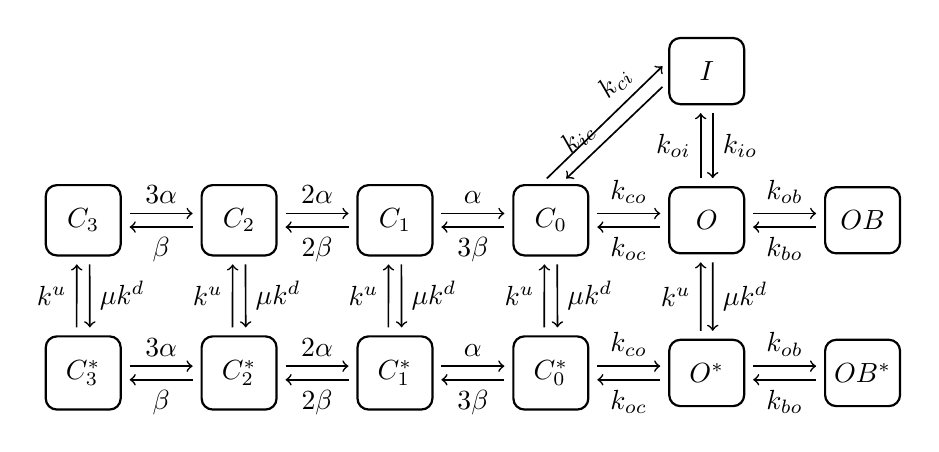
\begin{tikzpicture}[
   font=\sffamily,
   every matrix/.style={ampersand replacement=\&,column sep=1cm,row sep=1cm},
   state/.style={draw,thick,rounded corners,inner sep=.3cm},
   to/.style={->,semithick,shorten >=0.1cm,shorten <=0.1cm},
   Q/.style={->,semithick,sloped,pos=0.700000,shorten >=0.1cm,shorten <=0.1cm},  
   every node/.style={auto}]
\matrix{
\&\&\&\&\node[state] (I) {\parbox{10pt}{\centerline{$I$}}};\&\\
\node[state] (C_{3}) {\parbox{10pt}{\centerline{$C_{3}$}}};\&\node[state] (C_{2}) {\parbox{10pt}{\centerline{$C_{2}$}}};\&\node[state] (C_{1}) {\parbox{10pt}{\centerline{$C_{1}$}}};\&\node[state] (C_{0}) {\parbox{10pt}{\centerline{$C_{0}$}}};\&\node[state] (O) {\parbox{10pt}{\centerline{$O$}}};\&\node[state] (OB) {\parbox{10pt}{\centerline{$OB$}}};\\
\node[state] (C_{3}^{*}) {\parbox{10pt}{\centerline{$C_{3}^{*}$}}};\&\node[state] (C_{2}^{*}) {\parbox{10pt}{\centerline{$C_{2}^{*}$}}};\&\node[state] (C_{1}^{*}) {\parbox{10pt}{\centerline{$C_{1}^{*}$}}};\&\node[state] (C_{0}^{*}) {\parbox{10pt}{\centerline{$C_{0}^{*}$}}};\&\node[state] (O^{*}) {\parbox{10pt}{\centerline{$O^{*}$}}};\&\node[state] (OB^{*}) {\parbox{10pt}{\centerline{$OB^{*}$}}};\\
};
\draw[to]  (O^{*}.100) to node {$k^{u}$} (O.260);
\draw[to]  (O^{*}.10) to node {$k_{ob}$} (OB^{*}.170);
\draw[to]  (O^{*}.190) to node {$k_{oc}$} (C_{0}^{*}.350);
\draw[to]  (O.280) to node {$\mu k^{d}$} (O^{*}.80);
\draw[to]  (O.100) to node {$k_{oi}$} (I.260);
\draw[to]  (O.190) to node {$k_{oc}$} (C_{0}.350);
\draw[to]  (O.10) to node {$k_{ob}$} (OB.170);
\draw[to]  (I.280) to node {$k_{io}$} (O.80);
\draw[Q]  (I.195) to node {$k_{ic}$} (C_{0}.75);
\draw[to]  (C_{0}.10) to node {$k_{co}$} (O.170);
\draw[Q]  (C_{0}.105) to node {$k_{ci}$} (I.165);
\draw[to]  (C_{0}.190) to node {$3\beta$} (C_{1}.350);
\draw[to]  (C_{0}.280) to node {$\mu k^{d}$} (C_{0}^{*}.80);
\draw[to]  (C_{1}.10) to node {$\alpha$} (C_{0}.170);
\draw[to]  (C_{1}.190) to node {$2\beta$} (C_{2}.350);
\draw[to]  (C_{1}.280) to node {$\mu k^{d}$} (C_{1}^{*}.80);
\draw[to]  (C_{2}.10) to node {$2\alpha$} (C_{1}.170);
\draw[to]  (C_{2}.190) to node {$\beta$} (C_{3}.350);
\draw[to]  (C_{2}.280) to node {$\mu k^{d}$} (C_{2}^{*}.80);
\draw[to]  (C_{3}.10) to node {$3\alpha$} (C_{2}.170);
\draw[to]  (C_{3}.280) to node {$\mu k^{d}$} (C_{3}^{*}.80);
\draw[to]  (OB.190) to node {$k_{bo}$} (O.350);
\draw[to]  (OB^{*}.190) to node {$k_{bo}$} (O^{*}.350);
\draw[to]  (C_{0}^{*}.10) to node {$k_{co}$} (O^{*}.170);
\draw[to]  (C_{0}^{*}.100) to node {$k^{u}$} (C_{0}.260);
\draw[to]  (C_{0}^{*}.190) to node {$3\beta$} (C_{1}^{*}.350);
\draw[to]  (C_{1}^{*}.100) to node {$k^{u}$} (C_{1}.260);
\draw[to]  (C_{1}^{*}.10) to node {$\alpha$} (C_{0}^{*}.170);
\draw[to]  (C_{1}^{*}.190) to node {$2\beta$} (C_{2}^{*}.350);
\draw[to]  (C_{2}^{*}.100) to node {$k^{u}$} (C_{2}.260);
\draw[to]  (C_{2}^{*}.10) to node {$2\alpha$} (C_{1}^{*}.170);
\draw[to]  (C_{2}^{*}.190) to node {$\beta$} (C_{3}^{*}.350);
\draw[to]  (C_{3}^{*}.100) to node {$k^{u}$} (C_{3}.260);
\draw[to]  (C_{3}^{*}.10) to node {$3\alpha$} (C_{2}^{*}.170);
\end{tikzpicture}
\end{center}
\caption{Markov model of the mutant sodium channel with a blocker associated
with the open states. The model consists of the states $O,I,OB,C_{0}%
,C_{1},C_{2},$ and $C_{3}$ of the normal mode and $OB^*,O^{*},C^{*}_{0},C^{*}%
_{1},C^{*}_{2},$ and $C^{*}_{3}$ of the burst mode (lower part). The drug is
characterized by the two parameters $k_{bo}$ and $k_{ob}$.}%
\label{burstdrg}
\end{figure}

\newpage

%\subsection{Numerical experiments}
%\graytable{l}{
%{|c|c|} \hline
%$\mu$ & 30\\ \hline
%$k_{ob}$ &  0.2196 $\rm{ms^{-1}}$\\ \hline
%$k_{bo}$ &0.0001578 $\rm{ms^{-1}}$\\ \hline
%}{Values of the parameters used in the model in Figure \ref{burstdrg}.
%%\ref{burstdrg}. 
%The remaining rates are as in Table \ref{tab:burst_param}.
%}


In Figure \ref{NaB/pdf3_d.pdf}, we show the probability density functions of the wild type, the mutant (using $\mu=30$), and
the mutant case where the optimal open blocker is applied. The blocker repairs the effect of the mutation and the same effect is seen in Figure \ref{NaB/mc_d.pdf} where the currents are given; the open blocker removes the late sodium current.


\fig{NaB/pdf3_d.pdf}{Probability density functions for the wild type, the mutant ($\mu=30$), and the mutant in the presence of the open blocker. The subscripts $o$ and $n$ refer to open and non-conduction states, respectively, where the states are shown in  Figure \ref{burstdrg}.}
\fig{NaB/mc_d.pdf}{Currents computed using the Markov model given in Figure \ref{burstdrg}
for the wild type, the mutant ($\mu=30$), and the mutant in the presence of the open blocker.}

\clearpage

\section{Notes \label{notesburst}}

\begin{enumerate}
\item The burst mode is discussed by Bennett et al. \cite{Bennett1995} and modeled
in the paper by Clancy and Rudy \cite{Clancy1999}.
\item The form of the model illustrated in Figure \ref{burst} is taken from Clancy and
Rudy \cite{Clancy1999}, but the functions and parameters of the model are not
taken from their paper.
\item As mentioned above, the introduction of a burst mode is a convenient way of modeling the effect of certain mutations. The notion that gating may enter various modes has been considerably extended and studied in the papers by Chakrapani et al. \cite{ Chakrapani2007a, Chakrapani2007b, Chakrapani2011} and by Ionescu et al. \cite{Ionescu2007}. In the recent paper by Siekmann et al \cite{Siekmann2014} the concept of modal gating is studied and a method for detecting mode changes based on single channel data is developed.
\end{enumerate}

\chapter[Whole cell action potentials]{Action potentials: Summing up the effect of loads of ion channels}
\label{ap}

    In this final chapter we will use the theoretical drugs developed in various chapters above for whole cell simulations. So far we have studied very small parts of a cell. We started by studying the dynamics going on in a single dyad; see Figure \ref{cicr_1D}. The size of one dyad is
less than 1/1000 $\mu \mbox{m}^3$\cite{Bers2001} and we have been concerned with the concentration of calcium ions in this small volume. We have also studied the voltage dynamics in the vicinity of a single ion channel. The size of a single channel is about \GTLV{1 nm}. Now we address what is going on in a whole cell and it is important to realize that, compared to the single dyad and the single ion channel, the whole cell is huge; a normal ventricular cell is about 30,000 $\mu \mbox{m}^3$  \cite{Bers2001}, or on the order of  30 million times larger than the single dyad.

    In the analysis of single channels, we have regarded the state of a channel as a stochastic variable. In the whole cell, however, the effect of a huge number of channels is added and the sum can be modeled using deterministic equations. We will still use the same Markov model formalism in terms of reaction schemes to formulate the models, but now we will use the associated master equations (see page \pageref{master_equation}) to define the open probability of the channel. Thus we need to solve deterministic systems of ordinary differential equations to find the open probability as a function of time.

    Since the state of the channels will be represented using Markov model reaction schemes, we can study mutations in the same manner as we did for the single channel case. Therefore, we can use the results we derived above regarding optimal theoretical drugs for the single channel case for the whole cell case as well. The reasoning behind this was indicated earlier: If a mathematical model of a cell is constructed by using models of a huge number of single channels and we can repair the function of each single channel, the whole cell will be repaired.

    In this chapter we will start by introducing a model of the action potential of the whole cell. We will focus on a simplified model that will merely represent the action potential in a qualitatively relevant manner; it will not represent any particular action potential in a quantitatively correct manner.   Using numerical experiments, we will show that the model provides reasonable results for both wild type and various mutations. Finally, we will use the optimal theoretical drugs derived above and see that the effect of various mutations can be repaired using the theoretical drugs.

\section{Whole cell action potential model}
\label{sec:ap}


Our aim is now to introduce a reasonably simple action potential model for a whole cell. We will use the building blocks developed above and add some new features in order to get an action potential that is qualitatively reasonable.


\begin{figure}
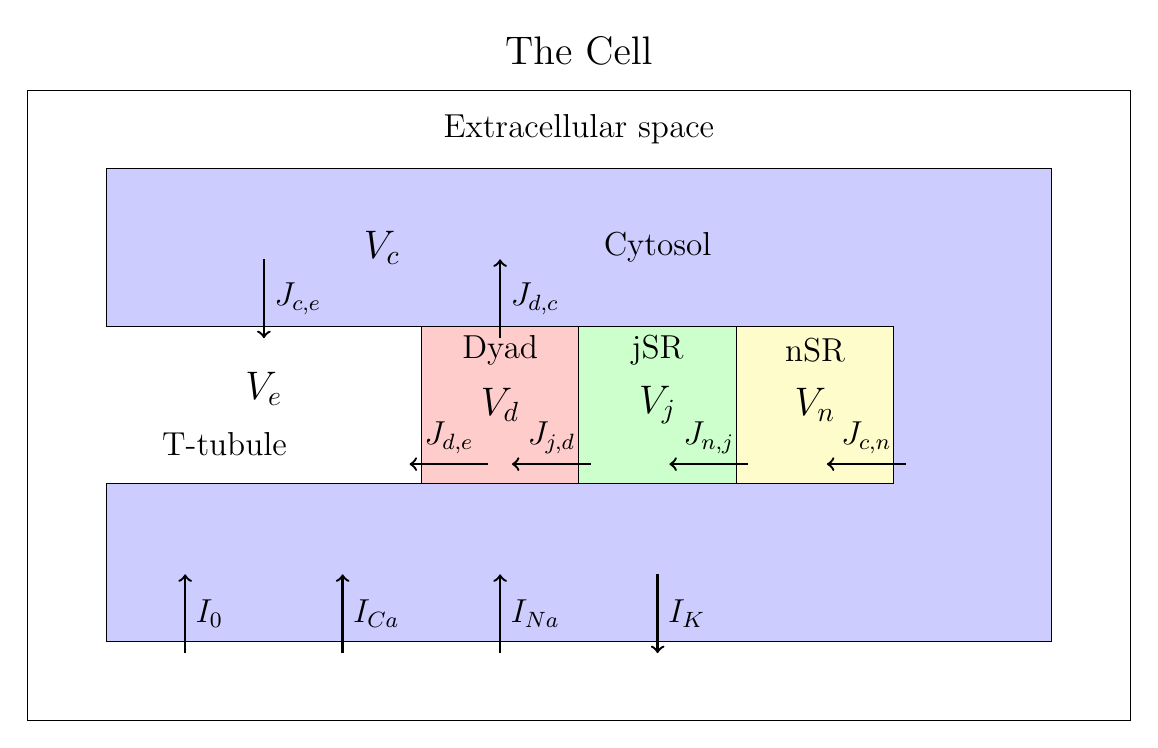
\begin{tikzpicture}[line width=0.3mm]
\tikzstyle{every node}=[font=\large]
\draw[line width=0,fill=white!80!white] (-1,-1) -- (13,-1) -- (13,7) -- (-1,7) -- (-1,-1);
\draw[line width=0,fill=white!80!blue] (0,0) -- (12,0) -- (12,6) -- (0,6)  -- (0,4) -- (10,4) -- (10,2) -- (0,2) -- (0,0);
\draw[line width=0,fill=white!80!yellow] (8,2) -- (10,2) -- (10,4) -- (8,4) -- (8,2);
\draw[line width=0,fill=white!80!green] (6,2) -- (8,2) -- (8,4) -- (6,4) -- (6,2);
\draw[line width=0,fill=white!80!red] (4,2) -- (6,2) -- (6,4) -- (4,4) -- (4,2);
\node[black!50!black] at (5, 3.0) {\Large{$V_{d}$}};
\node[black!50!black] at (7, 3.0) {\Large{$V_{j}$}};
\node[black!50!black] at (9, 3.0) {\Large{$V_{n}$}};
\node[black!50!black] at (5, 3.7) {Dyad};
\node[black!50!black] at (7, 3.7) {jSR};
\node[black!50!black] at (9, 3.7) {nSR};
\draw[->, black] (5,3.85) --node[right] {$J_{d,c}$} (5,4.85);
\draw[->, black] (2,4.85) --node[right] {$J_{c,e}$} (2,3.85);
\node[black!50!black] at (3.5, 5) {\Large{$V_{c}$}};
\node[black!50!black] at (2, 3.2) {\Large{$V_{e}$}};
\node[black!50!black] at (1.5, 2.5) {T-tubule};
\node[black!50!black] at (6, 6.5) {Extracellular space};
\node[black!50!black] at (7, 5) {Cytosol};
\node[black!50!black] at (6, 7.5) {\Large{The Cell}};
\draw[<-, black] (3.85,2.25) --node[above] {$J_{d,e}$} (4.85,2.25);
\draw[->, black] (6.15,2.25) --node[above] {$J_{j,d}$} (5.15,2.25);
\draw[->, black] (8.15,2.25) --node[above] {$J_{n,j}$} (7.15,2.25);
\draw[->, black] (10.15,2.25) --node[above] {$J_{c,n}$} (9.15,2.25);
\draw[->, black] (1,-0.15) --node[right] {$I_{0}$} (1,0.85);
\draw[->, black] (3,-0.15) --node[right] {$I_{Ca}$} (3,0.85);
\draw[->, black] (5,-0.15) --node[right] {$I_{Na}$} (5,0.85);
\draw[<-, black] (7,-0.15) --node[right] {$I_{K}$} (7,0.85);
%\draw[<->, black] (9,-0.15) --node[right] {$I_{NaK}$} (9,0.85);
\end{tikzpicture}
\caption{Sketch of the calcium dynamics and the fluxes and pumps involved. The volumes of the cytosol, the dyad, the junctional sarcoplasmic reticulum (JSR) and the network sarcoplasmic reticulum (NSR) are $V_c,\, V_d,\, V_j,$ and $V_n$, respectively.\label{fig:sketch}}
\end{figure}




The model consists of six main variables: $v, \, c_{e}, \, c_{c}, \, c_{d}, \, c_{j}$, and $c_{n}.$
Here $v,$ as usual, denotes the transmembrane potential given in mV. All the
other variables are concentrations given in $\mu$M; $c_{e}$ is the extracellular calcium concentration, $c_{c}$ is the cytosolic
concentration, $c_{d}$ is the concentration of the dyad, $c_{j}$ is the
concentration of the JSR, and finally $c_{n}$ is the concentration of the NSR;
see Figure \ref{fig:sketch}. In addition to these six main variables, we will have
variables associated with various Markov models; all these variables are between zero
and one; they also denote probabilities and they have no unit. The transmembrane
potential is governed by the equation
\begin{equation}
Cv^{\prime}=-\left(  I_{Na}+I_{Ca}+I_{K}+I_{0}\right)  \label{dvdt50}
\end{equation}
where the minus sign is according to convention in the field. Here $C$ denotes the
capacitance and is simply a constant that will be specified below. The current
$I_{0}$ represents a stimulus of the cell and we will use it below to initiate
action potentials. The sodium current $I_{Na},$ the calcium current $I_{Ca},$
and the potassium current $I_{K}$ need some attention and will be handled
separately.

\bigskip
In addition to the transmembrane potential, we need to keep track of
all five calcium concentrations.
%We will assume that the extracellular calcium concentration $c_{e}$ is given and that it is kept constant for all time; it will just enter as a paramter in the computations. But theconcentrations $c_{c},c_{d},c_{j}$ and $c_{n}$ must be updated dynamically.
By considering Figure \ref{fig:sketch}, we see that the cytosolic concentration can change in
three ways:\footnote{This is a major simplification; many other things can
happen to calcium but this rough description is sufficient for our purposes.
} (1) Calcium may diffuse into the cytosolic space from the
dyad,\footnote{It is important to recall here that when we talk about the dyad
now, we really refer to a space representing the sum of all the dyads of the
cell. So what used to be a very tiny place is not so tiny anymore.} leading to
an increase in the cytosolic concentrations; (2) it can be pumped from the cytosol into the
NSR and thereby reduce the cytosolic concentration; or, finally, (3) it can be
pumped out to the extracellular space, thereby reducing the cytosolic
concentration. The calcium concentration of the NSR, $c_{n},$ will be
increased as calcium is pumped into this space from the cytosol and reduced
by diffusion into its neighboring space, the JSR. In the JSR the calcium
concentration will increase through diffusion from the NSR and be reduced when
calcium is released through the ryanodine receptor (RyR) into the dyadic space. Finally, the
concentration in the dyad will increase when calcium is released from the JSR
to the dyad; it will be reduced as calcium diffuses out to the cytosol and
finally it will be increased when calcium is released into the dyad through
the L-type calcium channels (LCCs). In mathematical terms, we get the following system of
equations:
\begin{align}
V_{c}c_{c}^{\prime}  & =J_{d,c}-J_{c,n}-J_{c,e},\label{c51}\\
V_{n}c_{n}^{\prime}  & =J_{c,n}-J_{n,j},\label{c52}\\
V_{j}c_{j}^{\prime}  & =J_{n,j}-J_{j,d},\label{c53}\\
V_{d}c_{d}^{\prime}  & =J_{j,d}-J_{d,c}-J_{d,e}.\label{c54} \\
V_{e}c_{e}^{\prime}  & =J_{c,e}+J_{d,e}.\label{c55}
\end{align}
Here the notation $J_{x,y}$ denotes a flux of calcium from space $x$ to
space $y.$ So $J_{d,c}$ denotes the flux of calcium from the dyad ($d$) to
the cytosol ($c$) and, similarly, $J_{d,e}$ denotes the flux of calcium from
the  dyad ($d$)  to the extracellular ($e$) space. Here $V_{x}$ denotes the
volume fraction occupied by the space $x.$  The total amount of calcium in the system is given by
\begin{equation}
c=V_{c}c_{c}+V_{n}c_{n}+V_{j}c_{j}+V_{d}c_{d}+V_{e}c_{e}. \label{tot_ca}
\end{equation}



\subsection{Conservation of calcium}

%Suppose the cell membrane is completely closed so we have
%\begin{equation}
%J_{d,e}=J_{e,d}=0,
%\end{equation}
%then
It follows from the system (ref{c51})-(\ref{c55}) that
\begin{equation}
c^{\prime}=0,
\end{equation}
so the total amount of calcium is conserved no matter how the calcium
dynamics of the cell are organized.

%This observation motivates a modeling
%requirement for the fluxes across the cell membrane. We are modeling a
%process where the cell is supposed to be stimulated by a current, then undergo
%an action potential of length $T$, and then turn back to a normal resting
%state and wait for another stimulus.
%In general, we have
%\begin{equation}
%c^{\prime}=J_{e,d}-J_{d,e}
%\end{equation}
%and in order for the total calcium concentration to return to the same value
%after an action potential, we need to have
%\begin{equation}
%c(T)=c(0)
%\end{equation}
%\bigskip and this is satisfied if
%\begin{equation}
%\int_{0}^{T}J_{e,d}dt=\int_{0}^{T}J_{d,e}dt.\label{J_req}
%\end{equation}
%Below, we will make sure that we tune our parameters such that this requirement (at least approximately) is satisfied.


\subsection{Definition of calcium-related fluxes}

\begin{table}
\begin{center}
\begin{tabular}{|c|c|} \hline
$V_d$ & 0.1\% \\ \hline
$V_j$ & 0.3\% \\ \hline
$V_n$ & 1\% \\ \hline
$V_c$ & 98.6\% \\ \hline
\end{tabular}
\caption{The table shows the relative size of the intracellular spaces. Note that the volume fractions
of the intracellular space add up to $100\%$. In addition, $V_e$ represents $100\%$ of the extracellular space.
We assume that both the extracellular space and the total intracellular space are 30.4 pL
%The extracellular space is 30.4 pL and we assume that it equals the total intracellular space.
}
\end{center}
\end{table}

\begin{table}
\begin{center}
\begin{tabular}{|c|c|} \hline
$k_{c,n}$ & 0.01 \\ \hline
$k_{j,d}$ & 0.01 \\ \hline
$k_{d,c}$ & 0.001 \\ \hline
$k_{d,e}$ & 0.0001 \\ \hline
$k_{n,j}$ & 0.0001  \\ \hline
$k_{c,e}$ & 0.00001 \\ \hline
\end{tabular}
\caption{\label{tab:k}Constants used to define the fluxes between the different spaces. The constants are in units of 1/ms.
}
\end{center}
\end{table}

\begin{figure}[ptb]
\begin{center}
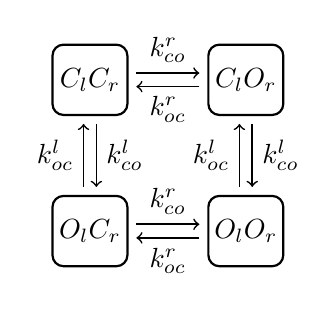
\begin{tikzpicture}[
   font=\sffamily,
   every matrix/.style={ampersand replacement=\&,column sep=1cm,row sep=1cm},
   state/.style={draw,thick,rounded corners,inner sep=.3cm},
   to/.style={->,semithick,shorten >=0.1cm,shorten <=0.1cm},
   Q/.style={->,semithick,sloped,pos=0.700000,shorten >=0.1cm,shorten <=0.1cm},
   every node/.style={auto}]
\matrix{
\node[state] (C_{l}C_{r}) {\parbox{10pt}{\centerline{$C_{l}C_{r}$}}};\&\node[state] (C_{l}O_{r}) {\parbox{10pt}{\centerline{$C_{l}O_{r}$}}};\\
\node[state] (O_{l}C_{r}) {\parbox{10pt}{\centerline{$O_{l}C_{r}$}}};\&\node[state] (O_{l}O_{r}) {\parbox{10pt}{\centerline{$O_{l}O_{r}$}}};\\
};
\draw[to]  (C_{l}C_{r}.10) to node {$k_{co}^{r}$} (C_{l}O_{r}.170);
\draw[to]  (C_{l}C_{r}.280) to node {$k_{co}^{l}$} (O_{l}C_{r}.80);
\draw[to]  (C_{l}O_{r}.190) to node {$k_{oc}^{r}$} (C_{l}C_{r}.350);
\draw[to]  (C_{l}O_{r}.280) to node {$k_{co}^{l}$} (O_{l}O_{r}.80);
\draw[to]  (O_{l}C_{r}.100) to node {$k_{oc}^{l}$} (C_{l}C_{r}.260);
\draw[to]  (O_{l}C_{r}.10) to node {$k_{co}^{r}$} (O_{l}O_{r}.170);
\draw[to]  (O_{l}O_{r}.100) to node {$k_{oc}^{l}$} (C_{l}O_{r}.260);
\draw[to]  (O_{l}O_{r}.190) to node {$k_{oc}^{r}$} (O_{l}C_{r}.350);
\end{tikzpicture}
\end{center}
\caption{Markov model including four possible states: $C_{l}C_{r}$ (both
closed), $C_{l}O_{r}$ (LCC closed, RyR open), $O_{l}O_{r}$ (both open), and
$O_{l}C_{r}$ (LCC open, RyR closed).}
\label{eq:m_rl2}
\end{figure}

%The states of this combined Markov model are given by $C_{l}C_{r}$ (both
%closed), $C_{l}O_{r}$ (LCC closed, RyR open), $O_{l}O_{r}$ (both open), and
%$O_{l}C_{r}$ (LCC open, RyR closed). In our computations, we use the rates shown in Table \ref{fundtions2}.

%following functions
%\begin{equation}
\begin{table}
\begin{center}
%\begin{tabular}[c]{|l|l|l|l|} \hline
%$k_{co}^{r}=\mu \frac{x^4}{K(y)^4+x^4}$ & $k_{oc}^{r}=1$ &
%$K(y) =  K_{max}-y/1000$ & $K_{max} = 7.4\mu$M \\ \hline
%$k_{co}^{l}=\eta\, l_{\infty}(V)/\tau_l$ & $k_{oc}^{l}=(1-l_{\infty}(V))/\tau_l%$ &$l_{\infty}(V) = 0.01 \exp(-(V-5)^2/500)$
%&$\tau_l=1$ms \\ \hline
\begin{tabular}[c]{|l|l|} \hline
RyR: & LCC: \\
$k_{co}^{r}(c_d,c_j)=\mu \frac{c_d^4}{K(c_j)^4+c_d^4} \text{ ms}^{-1}$ &$k_{co}^{l}(v)=\eta\, l_{\infty}(v)/\tau_l$ \\
$k_{oc}^{r}=1 \text{ ms}^{-1}$ & $k_{oc}^{l}(v)=(1-l_{\infty}(v))/\tau_l$ \\
$K(c_j) = 20+1000(\frac{1000-c_j}{600})^2$ &  $ l_{\infty}(v) = \exp(-(\frac{v-55}{10})^2)$ \\
 & $\tau_l=1$ ms\\ \hline
\end{tabular}
\end{center}
%\end{equation}
\caption{Reaction rates used in the Markov model illustrated in
Figure \ref{eq:m_rl2}.
As usual,  $\mu \ge 1$ denotes the mutation severity
index of the RyR and $\eta \ge 1$ denotes the mutation severity
index of the LCC. }
\label{functions2}
\end{table}

We need to define all the fluxes entering the system (ref{c51})-(\ref{c55}) and we start with the simple diffusion fluxes. Some of
them have been used in earlier chapters, but we need a little more notation
here, so we redefine all the terms.

\subsubsection{Flux $J_{d,c}$ from the dyad to the cytosol}
We assume that the pure diffusion flux
from the dyad to the cytosol can be written as
\begin{equation}
J_{d,c}=k_{d,c}\left(  c_{d}-c_{c}\right).
 \label{J_dc}
\end{equation}
Here we assume that $k_{d,c}$ is a constant and the value used in our computations is given in Table \ref{tab:k}.

\subsubsection{Flux $J_{n,j}$ from the NSR to the JSR}
Similarly, we assume that the diffusion flux from the NSR to the JSR can be written as
\begin{equation}
J_{n,j}=k_{n,j}\left(  c_{n}-c_{j}\right), \label{J_nj}
\end{equation}
where $k_{n,j}$ is assumed to be a constant (see Table \ref{tab:k}).

\subsubsection{RyR flux $J_{j,d}$ from the JSR to the dyad}
The
flux from the JSR to the dyad can be written in the form
\begin{equation}
J_{j,d}=o_{j,d}k_{j,d}\left(  c_{j}-c_{d}\right), \label{J_jd}
\end{equation}
where, as usual, $o_{j,d}$ is governed by a Markov model and $k_{j,d}$ is a
constant giving the speed of diffusion when the RyR channel (situated between
the JSR and the dyad) is open.

The variable $o_{j,d}$ is governed by the Markov model
used in Chapter \ref{cicr}. For convenience the Markov model is repeated here in Figure \ref{eq:m_rl2} and  the functions
used in the model are given in Table \ref{functions2}. Note that $o_{j,d}$ is the probability of being in the state $C_lO_r$ or the state $O_lO_r$ of the Markov model given in Figure \ref{eq:m_rl2}.

%The parameters and functions are unaltered, except for $K(y)$
%the halv-saturation constant
%which has been changed to:
%\begin{equation}
%K(y) = 20+1000(\frac{1000-y}{600})^2. \label{halfmax}
%\end{equation}

%have been adapted to the current setting:
%illustrated in Figure xxx and the associated system of ordinary differential equations are given by xxx:
%\textbf{GTL: Insert the Markov model (ode-system and Figure) that you actually use.}



\subsubsection{Flux from the extracellular space to the dyad: $J_{d,e}$}

 This flux was introduced above (see page \pageref{GHK}) and referred to as the Goldman-Hodgkin-Katz (GHK) flux. In the present notation, we write

\begin{equation}
J_{d,e}=o_{d,e} k_{d,e} \frac{c_d-c_{e}e^{-\frac{v}{v_0}}}{1-e^{-\frac{v}{v_0}}}\frac{v}{v_0}.\label{J_ed}
\end{equation}
\graytable{l}{
{|c|c|} \hline
$F$ & $96485.3$ C mol$^{-1}$\\ \hline
$R$ & $8.3145$ J mol$^{-1}$K$^{-1}$\\\hline
$T$ & 310 K\\\hline
$v_0$ & 13.357 mV\\ \hline
}{Parameters in (\ref{J_ed}).\label{FRT_ed}}
Here %$D$ is Fick's diffusion constant,
$F$ is Faraday's constant, $R$ is the gas constant,
and $T$ is the absolute temperature and we have defined
\[
v_0=\frac{RT}{2F}.
\]
 The parameters involved in defining the $J_{d,e}$ flux are given in Table \ref{FRT_ed}. Furthermore, $o_{d,e}$ is governed by the Markov model
 given in Figure \ref{eq:m_rl2}. Here $o_{d,e}$ is the probability of being in the state $O_lC_r$ or the state $O_lO_r$ of the Markov model
  in Figure \ref{eq:m_rl2}.




%\[ l_{\infty}(v) = \exp(-(\frac{v-55}{10})^2). \]
%}
%presented in Figure xxx. The associated system of ordinary differential equations is given by xxxGTLxxx.
%xxx. \textbf{GTL: Insert the LCC model (ode-system and Figure) that you
%actually use (I do not if you want to couple the two models or treat them
%separately (LCC and RYR).}




\subsection{Definition of calcium pumps}


The terms $J_{c,e}$ and $J_{c,n}$ remain to be defined. These terms are active
fluxes, or pumps, that continuously remove calcium from the cytosol
and out to the extracellular domain $(J_{c,e})$ and into the NSR $(J_{c,n}).$
These pumps transport calcium against a considerable concentration gradient and
the operation therefore requires energy. In our model we do not track the
energy consumption and we simply introduce the pumps:
\begin{equation}
J_{c,e}=k_{c,e} (c_c-c_e/18000)  \label{J_ce}
\end{equation}
and
\begin{equation}
J_{c,n}= k_{c,n} (c_c-c_n/10000).  \label{J_cn}
\end{equation}


%xxx \textbf{GTL: insert the pumps you are using (follow the notational convention).}

\subsection{Definition of the currents}

The currents $I_{Na},\, I_K$ and $I_{Ca}$ of (\ref{dvdt50}) remain to be defined. Each current will be written in the form
\[
I_x=o_x g_x (v-v_x),
\]
where  $o_x$ is the open probability of the channel given by the continuous version of a Markov model, $g_x$ is the maximum conductance of the channel, and $v_x$ is the resting potential.

\subsubsection{Sodium current $I_{Na}$}

The sodium current has been studied above; see Chapters \ref{simple_Na} and \ref{burst_chap}. The model takes the form
\begin{equation}
I_{Na}= o_{Na} g_{Na}(v-v_{Na}),   \label{J_Na}
\end{equation}
where the open probability $o_{Na}$ is the sum of the probability of being in the $O$ or the $O^*$ state of the Markov model of Figure  \ref{wtreac3300}.

\begin{figure}[ptb]
\begin{center}
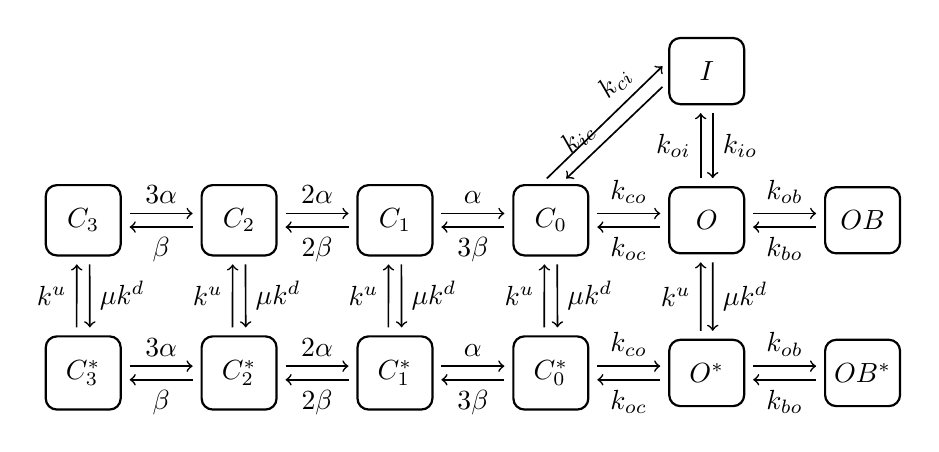
\begin{tikzpicture}[
   font=\sffamily,
   every matrix/.style={ampersand replacement=\&,column sep=1cm,row sep=1cm},
   state/.style={draw,thick,rounded corners,inner sep=.3cm},
   to/.style={->,semithick,shorten >=0.1cm,shorten <=0.1cm},
   Q/.style={->,semithick,sloped,pos=0.700000,shorten >=0.1cm,shorten <=0.1cm},
   every node/.style={auto}]
\matrix{
\&\&\&\&\node[state] (I) {\parbox{10pt}{\centerline{$I$}}};\&\\
\node[state] (C_{3}) {\parbox{10pt}{\centerline{$C_{3}$}}};\&\node[state] (C_{2}) {\parbox{10pt}{\centerline{$C_{2}$}}};\&\node[state] (C_{1}) {\parbox{10pt}{\centerline{$C_{1}$}}};\&\node[state] (C_{0}) {\parbox{10pt}{\centerline{$C_{0}$}}};\&\node[state] (O) {\parbox{10pt}{\centerline{$O$}}};\&\node[state] (OB) {\parbox{10pt}{\centerline{$OB$}}};\\
\node[state] (C_{3}^{*}) {\parbox{10pt}{\centerline{$C_{3}^{*}$}}};\&\node[state] (C_{2}^{*}) {\parbox{10pt}{\centerline{$C_{2}^{*}$}}};\&\node[state] (C_{1}^{*}) {\parbox{10pt}{\centerline{$C_{1}^{*}$}}};\&\node[state] (C_{0}^{*}) {\parbox{10pt}{\centerline{$C_{0}^{*}$}}};\&\node[state] (O^{*}) {\parbox{10pt}{\centerline{$O^{*}$}}};\&\node[state] (OB^{*}) {\parbox{10pt}{\centerline{$OB^{*}$}}};\\
};
\draw[to]  (O^{*}.100) to node {$k^{u}$} (O.260);
\draw[to]  (O^{*}.10) to node {$k_{ob}$} (OB^{*}.170);
\draw[to]  (O^{*}.190) to node {$k_{oc}$} (C_{0}^{*}.350);
\draw[to]  (O.280) to node {$\mu k^{d}$} (O^{*}.80);
\draw[to]  (O.100) to node {$k_{oi}$} (I.260);
\draw[to]  (O.190) to node {$k_{oc}$} (C_{0}.350);
\draw[to]  (O.10) to node {$k_{ob}$} (OB.170);
\draw[to]  (I.280) to node {$k_{io}$} (O.80);
\draw[Q]  (I.195) to node {$k_{ic}$} (C_{0}.75);
\draw[to]  (C_{0}.10) to node {$k_{co}$} (O.170);
\draw[Q]  (C_{0}.105) to node {$k_{ci}$} (I.165);
\draw[to]  (C_{0}.190) to node {$3\beta$} (C_{1}.350);
\draw[to]  (C_{0}.280) to node {$\mu k^{d}$} (C_{0}^{*}.80);
\draw[to]  (C_{1}.10) to node {$\alpha$} (C_{0}.170);
\draw[to]  (C_{1}.190) to node {$2\beta$} (C_{2}.350);
\draw[to]  (C_{1}.280) to node {$\mu k^{d}$} (C_{1}^{*}.80);
\draw[to]  (C_{2}.10) to node {$2\alpha$} (C_{1}.170);
\draw[to]  (C_{2}.190) to node {$\beta$} (C_{3}.350);
\draw[to]  (C_{2}.280) to node {$\mu k^{d}$} (C_{2}^{*}.80);
\draw[to]  (C_{3}.10) to node {$3\alpha$} (C_{2}.170);
\draw[to]  (C_{3}.280) to node {$\mu k^{d}$} (C_{3}^{*}.80);
\draw[to]  (OB.190) to node {$k_{bo}$} (O.350);
\draw[to]  (OB^{*}.190) to node {$k_{bo}$} (O^{*}.350);
\draw[to]  (C_{0}^{*}.10) to node {$k_{co}$} (O^{*}.170);
\draw[to]  (C_{0}^{*}.100) to node {$k^{u}$} (C_{0}.260);
\draw[to]  (C_{0}^{*}.190) to node {$3\beta$} (C_{1}^{*}.350);
\draw[to]  (C_{1}^{*}.100) to node {$k^{u}$} (C_{1}.260);
\draw[to]  (C_{1}^{*}.10) to node {$\alpha$} (C_{0}^{*}.170);
\draw[to]  (C_{1}^{*}.190) to node {$2\beta$} (C_{2}^{*}.350);
\draw[to]  (C_{2}^{*}.100) to node {$k^{u}$} (C_{2}.260);
\draw[to]  (C_{2}^{*}.10) to node {$2\alpha$} (C_{1}^{*}.170);
\draw[to]  (C_{2}^{*}.190) to node {$\beta$} (C_{3}^{*}.350);
\draw[to]  (C_{3}^{*}.100) to node {$k^{u}$} (C_{3}.260);
\draw[to]  (C_{3}^{*}.10) to node {$3\alpha$} (C_{2}^{*}.170);
\end{tikzpicture}
\end{center}
\caption{This figure is a copy of Figure \ref{burstdrg} and it illustrates a Markov model of the mutant sodium channel.
 The model consists of the states $O,I,OB,C_{0}
,C_{1},C_{2},$ and $C_{3}$ of the normal mode and $OB^*,O^{*},C^{*}_{0},C^{*}
_{1},C^{*}_{2},$ and $C^{*}_{3}$ of the burst mode (lower part). }
\label{wtreac3300}
\end{figure}

\subsubsection{Potassium current $I_{K}$}

The potassium current is written in the form
\begin{equation}
I_{K}= (o_{K} g_{K}(v) + g_{K1}(v)) (v-v_{K}),   \label{J_K}
\end{equation}
where the open probability $o_{K}$ is given by the Markov model of Figure  \ref{K1} with rates
\begin{align*}
\alpha(v) &  = e^{-7+0.03v},\\
\beta(v) &  = e^{-8-0.03v}. \\
\end{align*}
The voltage-dependent conductances are given by
\begin{align*}
g_K(v) &=  0.1 e^{-0.03v}, \\
g_{K1}(v) &= \frac{1}{1+e^{0.1 v+10}}. \\
\end{align*}


\begin{figure}[ptb]
\begin{center}
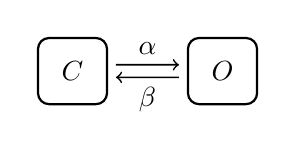
\begin{tikzpicture}[
   font=\sffamily,
   every matrix/.style={ampersand replacement=\&,column sep=1cm,row sep=1cm},
   state/.style={draw,thick,rounded corners,inner sep=.3cm},
   to/.style={->,semithick,shorten >=0.1cm,shorten <=0.1cm},
   Q/.style={->,semithick,sloped,pos=0.700000,shorten >=0.1cm,shorten <=0.1cm},
   every node/.style={auto}]
\matrix{
\node[state] (C) {$C$};\&\node[state] (O) {$O$};\\
};
\draw[to]  (O.190) to node {$\beta$} (C.350);
\draw[to]  (C.10) to node {$\alpha$} (O.170);
\end{tikzpicture}
\end{center}
\caption{Markov model of a potassium channel
consisting of one closed and one open state. }
\label{K1}
\end{figure}


\subsubsection{Calcium current $I_{Ca}$}

The calcium current is given by the calcium flux  $J_{d,e}$ from the dyad to the extracellular space plus the flux $J_{c,e}$ from the cytosol to the extracellular space.
In order to use these fluxes  in the equation governing the transmembrane potential, we need convert to current density,
\begin{equation}
I_{Ca}= 2 F\frac{V}{A} (-J_{d,e}-J_{c,e}).   \label{I_Ca}
\end{equation}
Here $V=30.4$ pL is the cell volume and $A=1.4\cdot 10^{-4} \text{ cm}^2$ is the cell area.

\subsection[Markov models as ODEs]{Markov models in terms of systems of differential equations}

The model of the action potential for a whole cell is a system of ordinary differential equations. For parts of the system this is clear from the equations,
but for the Markov models, this may seem unclear. In Section \ref{me_eq} we explained how to formulate a system of ordinary differential equation associated with the reaction scheme defining a Markov model.  Since the Markov models considered in the present chapter are considerably more complex, we will give one more example of this transition in order to clarify matters. To this end, consider the Markov model presented in Figure \ref{wtreac3331}.
 The associated system of ordinary differential equations governing the probabilities is given by
\begin{align*}
o^{\prime}  & =k_{io}i+k_{co}c_{0}-\left(  k_{oc}+k_{oi}\right)  o,\\
i^{\prime}  & =k_{oi}o+k_{ci}c_{0}-\left(  k_{io}+k_{ic}\right)  i,\\
c_{0}^{\prime}  & =k_{oc}o+k_{ic}i+\alpha c_{1}-\left(  k_{co}+k_{ci}
+3\beta\right)  c_{0},\\
c_{1}^{\prime}  & =3\beta c_{0}+2\alpha c_{2}-\left(  2\beta+\alpha\right)
c_{1},\\
c_{2}^{\prime}  & =2\beta c_{1}+3\alpha c_{3}-\left(  2\alpha+\beta\right)
c_{2},\\
c_{3}^{\prime}  & =\beta c_{2}-3\alpha c_{3}.
\end{align*}
Here, $o$ denotes the open probability of the sodium channel,  $c_0$ is the probability of the $C_0$ state, and so forth. Ideally, we would write $o_{Na}$ for $o$, $c_{0,Na}$ for $c_0$, and so forth, but it becomes clumsy. Since these variables represent probabilities, they sum to one (for all time) and we can therefore reduce the number of unknowns in the system by one.

Based on this example, it should be straightforward to formulate the system of ordinary differential equations associated with the more complex Markov model given in Figure \ref{wtreac3300}.

\begin{figure}[ptb]
\begin{center}
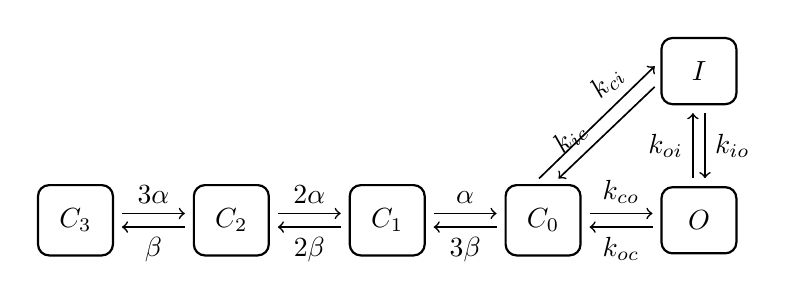
\begin{tikzpicture}[
   font=\sffamily,
   every matrix/.style={ampersand replacement=\&,column sep=1cm,row sep=1cm},
   state/.style={draw,thick,rounded corners,inner sep=.3cm},
   to/.style={->,semithick,shorten >=0.1cm,shorten <=0.1cm},
   Q/.style={->,semithick,sloped,pos=0.700000,shorten >=0.1cm,shorten <=0.1cm},
   every node/.style={auto}]
\matrix{
\&\&\&\&\node[state] (I) {\parbox{10pt}{\centerline{$I$}}};\\
\node[state] (C_{3}) {\parbox{10pt}{\centerline{$C_{3}$}}};\&\node[state] (C_{2}) {\parbox{10pt}{\centerline{$C_{2}$}}};\&\node[state] (C_{1}) {\parbox{10pt}{\centerline{$C_{1}$}}};\&\node[state] (C_{0}) {\parbox{10pt}{\centerline{$C_{0}$}}};\&\node[state] (O) {\parbox{10pt}{\centerline{$O$}}};\\
};
\draw[to]  (O.100) to node {$k_{oi}$} (I.260);
\draw[to]  (O.190) to node {$k_{oc}$} (C_{0}.350);
\draw[to]  (I.280) to node {$k_{io}$} (O.80);
\draw[Q]  (I.195) to node {$k_{ic}$} (C_{0}.75);
\draw[to]  (C_{0}.10) to node {$k_{co}$} (O.170);
\draw[Q]  (C_{0}.105) to node {$k_{ci}$} (I.165);
\draw[to]  (C_{0}.190) to node {$3\beta$} (C_{1}.350);
\draw[to]  (C_{1}.10) to node {$\alpha$} (C_{0}.170);
\draw[to]  (C_{1}.190) to node {$2\beta$} (C_{2}.350);
\draw[to]  (C_{2}.10) to node {$2\alpha$} (C_{1}.170);
\draw[to]  (C_{2}.190) to node {$\beta$} (C_{3}.350);
\draw[to]  (C_{3}.10) to node {$3\alpha$} (C_{2}.170);
\end{tikzpicture}
\end{center}
\caption{Markov model of a wild type sodium channel consisting of an open
state $(O)$, an inactivated state $(I)$, and four closed states $(C_{0}
,C_{1},C_{2}, \text{ and }C_{3})$. }
\label{wtreac3331}
\end{figure}


\section[Numerical action potential; wild type]{Numerical simulations using the action potential model for wild type Markov models}

The complete version of the model presented above can be written in the compact form
\begin{align}
Cv^{\prime}  & =-\left(  I_{Na}+I_{Ca}+I_{K}+I_{0}\right),  \label{s401}\\
u^{\prime}  & =F(v,u)\label{s402},
\end{align}
where $v$ is the transmembrane potential and all other variables are gathered in the vector $u$. The initial conditions used in the simulations are given in Table \ref{tab:init}. In addition, we need to specify the applied current $I_0$. This current will be zero most of the time, but it will be turned on every 500 ms in order to mimic periodic stimulation of the cell. More specifically,
we hold $I_0$ = -6 mV/ms for 5 ms at the start of each cycle.

\begin{table}
\begin{center}
\begin{tabular}{|c|c|} \hline
$v$ & -85 mV \\ \hline
$c_{d}$ & 0.1 $\mu$M \\ \hline
$c_{c}$ & 0.1 $\mu$M \\ \hline
$c_{j}$ & 1000 $\mu$M \\ \hline
$c_{n}$ & 1000 $\mu$M \\ \hline
$c_{e}$ & 1800 $\mu$M \\ \hline
\end{tabular}
\caption{Initial conditions. The Markov models for the LCC and RyR were initially set to closed and the Markov model for sodium channel was set to be in the state $C_3$. Starting with these conditions, the code is run for 1000 cycles in order to generate the initial conditions used in generating the figures below. The exact numbers obtained depend upon the chosen cycle length. \label{tab:init}}
\end{center}
\end{table}





\subsection{Single action potential}

In Figure \ref{ap:single1} we show the transmembrane potential and all the calcium concentration for a single action potential. There are a number of interesting effects acting together to generate the action potential. Let us consider some of them in some detail.

FIGURE: [fig/ap_single1.pdf, width=500 frac=0.8] The action potential of the model described in the present chapter. The membrane potential (upper left) and the dynamics of the five calcium concentrations are shown for 500 ms. The action potential is initiated by holding $I_0$ = -6 mV/ms for 5 ms. All variables return to their resting values after about 500 ms.  label{ap:single1}

FIGURE: [fig/ap_single2.pdf, width=500 frac=0.8] The first 20 ms of the simulation shown in Figure \ref{ap:single1}. Note the log scale in the upper right panel. There we see a slow rise due to the LCC opening, followed by a fast rise due to the RyR opening. label{ap:single2}

In Figure \ref{ap:single2} we show the first 20 ms of the computation. In the left panel we show the transmembrane potential $v$ (upper left panel), the open probability $o_{Na}$ (middle left panel), and the sodium current $I_{Na}$ (lower left panel). Observe that when the cell is stimulated by the applied current $I_0$, the transmembrane potential increases. This increase leads to an increased open probability of the sodium channel. When the sodium channel opens, the sodium current becomes large (or very negative, to be precise), which leads to a fast increase of the transmembrane potential. As the transmembrane potential reaches its peak value (at about 15 ms), the open probability starts to decline, since the channel inactivates. In the three right panels, we show the calcium concentration of the dyad $c_d$ (upper right panel), the calcium flux $J_{d,e}$ (middle right panel), and the open probability of the RyR channel  (lower right panel). We see that when the transmembrane potential starts increasing, the calcium flux $J_{d,e}$ increases and the calcium concentration of the dyad increases. This increase leads to the increased open probability (lower right panel) of the RyR channel and therefore the dyad concentration increases rapidly.

In Figure \ref{ap:single3}, we show the return to the stable equilibrium solution. In the left panel, we show the transmembrane (upper left panel), the open probability of the LCC (middle left panel), and the open probability of the gated potassium channel. After the sodium channel has switched off (see Figure \ref{ap:single2}), the calcium current contributes to a continued depolarized state. However, after about 20 ms the transmembrane potential starts declining because of a substantial (positive) potassium current.
%the open probability $o_{Na}$ (middle left panel), and the potassium current $I_K$ (lower left panel). We see that the sodium channel now is not conducting since $o_{Na}$ is almost zero. The transmembrane potential is reduced and this is due to a substantial (positive) potassium current.

In the right panels, we follow the development of the calcium concentration of the dyad $c_d$ (upper right panel),  the calcium concentration
\GTLV{$c_j$ of the JSR},
%$c_n$ of the NSR
(middle right panel), and the open probability of the RyR channel, denoted $o_{j,d}$ (lower right panel).
%\GTLV{we see that the jSR consentration falls rapidly when channel is open. This causes the channel to close, due an incrase in the half-maximum  constant (see
%$equation \ref{halfmax})}.
%We see that the dyad concentration is reduced and that the RyR is practically closed. The increase of the calcium concentration in the NSR is due to the pump $J_{c,n}$ and to the fact that the RyR channel is closed.

FIGURE: [fig/ap_single3.pdf, width=500 frac=0.8] After about 15 ms, the transmembrane potential (upper left) reaches its peak value and enters the plateau phase before it starts to decline toward the stable equilibrium solution.  label{ap:single3}

\subsection{Many action potentials}

In Figure \ref{ap:multiple}, we show the action potential for a simulation running for 25,000 ms. The left panel shows the transmembrane potential $v$ (upper left panel), the calcium concentration $c_d$ of the dyad (middle left panel), and the extracellular calcium concentration $c_e$ (lower left panel). From top to bottom in the right panels, we show the cytosolic calcium concentration $c_c$, the NSR calcium concentration $c_n$, and finally the JSR calcium concentration $c_j$. All variables return to their initial values and the rhythm seems to be perfect.
%In Figure xxx5, we show exactly the same variables after 10000 action potentials and it looks exactly the same.

FIGURE: [fig/ap_multiple.pdf, width=500 frac=0.8] The action potential running for 25,000 ms (50 beats). All variables return to their equilibrium values before a new action potential is initiated (every 500 ms).  label{ap:multiple}

\section[Changing the mean open time]{Changing the mean open time of the sodium channel while keeping the equilibrium probability fixed changes the action potential}
\label{sec:ap_mot}

We consider a case where we multiply all rates of the Markov model (see Figure \ref{wtreac3300}) of the sodium channel by the same factor. Here we use the wild type case ($\mu=1$) and the drug parameters ($k_{ob}, k_{bo}$) are set to zero. This will change the mean open time, but not the equilibrium probabilities. The results are given in Figure \ref{ap:mot}, where the blue line illustrates the results using default parameters, the red line represents the solution when all the rates are multiplied by 1.3, and finally the green line represents the solution when all the rates are multiplied by 0.7. We observe that the action potential changes substantially when the rates are changed (and the mean open time is changed), even though the equilibrium probabilities are kept unchanged.

FIGURE: [fig/ap_mot.pdf, width=500 frac=0.8] Slower dynamics (green) lead to later inactivation, yielding a higher plateau. Quicker dynamics (red) lead to faster recovery from inactivation, allowing a stronger late current.  label{ap:mot}


\section[Numerical action potential; mutations]{Numerical simulations using the action potential model when the cell is affected by a mutation}

We will use the model of the action potential for the whole cell introduced above to study the effect of mutations. We have studied many different theoretical models of mutations earlier, but here we will limit ourselves to study the effect of one theoretical model of a sodium channel mutation, one model of a RyR mutation, and one model of an LCC mutation. We will also see how the theoretical drugs derived above handle these mutations.




\subsection{Mutation of the sodium channel}

We consider a mutation of the sodium channel of the form presented in Figure \ref{wtreac3300}.
In Figure \ref{ap:burst_mut} we show simulation results comparing the wild type ($\mu=1$, blue),
the mutant ($\mu=10$, green), and a simulation (red) where  a drug is applied to the mutant case.
The Markov model describing the open state drug is given
in Figure \ref{wtreac3300}, where we have used drug parameters given by
\[
k_{bo} = k_{io}, \mbox{\ and \ }
k_{ob}=\left(  \mu-1\right)  \frac{k^{d}k^{u}k_{oi}}{\left(  k^{u}+\mu
k^{d}\right)  \left(  k^{u}+k^{d}\right)  };
\]
see (\ref{na_drug_ob}) and (\ref{na_drug_bo}).
As in the single channel case, we observe that the theoretical drug is able to repair the effect of the mutation.


FIGURE: [fig/ap_burst_mut.pdf, width=500 frac=0.8] The figure shows the action potential of the wild type (blue), the mutant (green), and the
mutant after the application of the drug (red). label{ap:burst_mut}

\subsection{Mutation of the RyR}

In Figure \ref{ap:ryr_mut} we have simulated mutation in the RyR using the Markov model given in Figure \ref{eq:m_rl2}. The figure shows the
wild type (blue, $\mu=1$), the mutant (green, $\mu=3$), and the mutant where the drug has been applied (red). We have used a closed state drug  computed as described in (\ref{closed_drg}) and (\ref{optimal_closed_charac}) and we observe that the theoretical drug is able to repair the effect of the mutation.
%{\bf xxxGTL: Is this a RyR mutation?  If RYR- what is the Markov model with drugs? Refs to model}






FIGURE: [fig/ap_ryr_mut.pdf, width=500 frac=0.8] The cytosolic calcium concentration for wild type (blue, $\mu=1$), the mutant (green, $\mu=3$), and the mutant after the application of the drug (red). We have used a closed state drug  as defined in (\ref{closed_drg}) with $k_{bc}=0.5$ ms$^{-1}$ and $k_{cb}=(\mu-1)k_{bc}$; see (\ref{optimal_closed_charac}).  label{ap:ryr_mut}

\subsection{Mutation of the LCC}

In Figure \ref{ap:lcc_mut} we have simulated mutation in the LCC channel, using $\eta=3$.
%{\bf xxxGTL: Is this a LCC mutation?  If LCC- what is the Markov model with drugs? Refs to model}
We model the mutation and the drug as defined in (\ref{closed_drg}) and (\ref{optimal_closed_charac}). As usual, $k_{bc}$ is a free parameter that must be chosen sufficiently large. Again, we note that the theoretical drug repairs the effect of the mutation.

FIGURE: [fig/ap_lcc_mut.pdf, width=500 frac=0.8] LCC mutation. The cytosolic calcium concentration for the wild type (blue, $\eta=1$), the mutant (green $\eta=3$), and the mutant case where the theoretical drug is applied (red). In the computations we have used $k_{bc}=0.05$ ms$^{-1}$; for larger values of $k_{bc}$ the results overlap with the wild type case. label{ap:lcc_mut}


\section{Notes}

\begin{enumerate}
\item The action potential model discussed in Section \ref{sec:ap} and used throughout this chapter is only of qualitative relevance; no effort is made to mimic the properties of one particular cell. The field of models for the action potential is huge and growing. A great collection of models is provided by the Auckland Bioengineering Institute at the University of Auckland and their collaborators; see CellML.org. Recent models tend to be increasingly complex and hard to deal with from a mathematical perspective, but clearly the models become more and more realistic in terms of mimicking the properties of the actual action potential.  As mentioned earlier, there are comprehensive introductions to the cardiac action potential, such as Rudy \cite{Rudy2012} and Rudy and Silva \cite{Rudy2006}.
\item In these notes we have used Matlab as the computational platform for all our simulations. For solving ordinary differential equations we have used the ODE15s function. However, solving the ordinary differential equations modeling the single cell action potential has received a great deal of attention and numerical methods suited for this problem have been developed. An early alternative was developed by Rush and Larsen \cite{Rush1978}; the method was improved to second by Sundnes et al.  \cite{Sundnes2009} and comparisons of several methods were provided by Marsh et al. \cite{Marsh2012} and Campos et al. \cite{Campos2013}; see also Stary and Biktashev \cite{Stary2015}. From a programming perspective, the explicit Euler scheme is always an attractive alternative, but for stiff problems the stability requirement often excludes that method. For instance, if we use the explicit Euler method with a fixed time step to compute the solutions shown in  Figure \ref{ap:single1}, we need about 26000 time-steps, whereas the ODE15s method needs 335 time steps.

\end{enumerate}

%\input{Potassium_L/blocker}
%\input{Potassium_L/K}


%\bibliographystyle{unsrt}
\bibliographystyle{plain}
\bibliography{ln}
\end{document}
